\chapter{Matrices and Determinants}
\label{ch_matrices_dets}
\section{Matrix operations}
\label{s_matop}

A matrix is a rectangular array of numbers. Here is an example of an
$m\times n$ matrix.
\[
A=\left[\matrix{
a_{1,1}      &a_{1,2}   &\cdots        &a_{1,n}\cr
a_{2,1}      &a_{2,2}   &\cdots        &a_{2,n}\cr
\vdots       &\vdots	&              &\vdots \cr
a_{m,1}      &a_{m,2}   &\cdots        &a_{m,n}\cr
}\right]
\]
This is sometimes abbreviated $A=[a_{i,j}]$.  An $m\times 1$ matrix is
called a column vector and a $1\times n$ matrix is called a row
vector. (The convention is that $m\times n$ means $m$ rows and $n$
columns).

Addition and scalar multiplication are defined for matrices exactly as
for vectors. If $s$ is a number
\[
s\left[\matrix{
a_{1,1}      &a_{1,2}   &\cdots        &a_{1,n}\cr
a_{2,1}      &a_{2,2}   &\cdots        &a_{2,n}\cr
\vdots       &\vdots	&              &\vdots \cr
a_{m,1}      &a_{m,2}   &\cdots        &a_{m,n}\cr
}\right]
=
\left[\matrix{
sa_{1,1}      &sa_{1,2}   &\cdots        &sa_{1,n}\cr
sa_{2,1}      &sa_{2,2}   &\cdots        &sa_{2,n}\cr
\vdots       &\vdots	&              &\vdots \cr
sa_{m,1}      &sa_{m,2}   &\cdots        &sa_{m,n}\cr
}\right],
\]
and
\[
\left[\matrix{
a_{1,1}      &a_{1,2}   &\cdots        &a_{1,n}\cr
a_{2,1}      &a_{2,2}   &\cdots        &a_{2,n}\cr
\vdots       &\vdots	&              &\vdots \cr
a_{m,1}      &a_{m,2}   &\cdots        &a_{m,n}\cr
}\right]
+
\left[\matrix{
b_{1,1}      &b_{1,2}   &\cdots        &b_{1,n}\cr
b_{2,1}      &b_{2,2}   &\cdots        &b_{2,n}\cr
\vdots       &\vdots	&              &\vdots \cr
b_{m,1}      &b_{m,2}   &\cdots        &b_{m,n}\cr
}\right]
=
\left[\matrix{
a_{1,1}+b_{1,1}      &a_{1,2}+b_{1,2}   &\cdots        &a_{1,n}+b_{1,n}\cr
a_{2,1}+b_{2,1}      &a_{2,2}+b_{2,2}   &\cdots        &a_{2,n}+b_{2,n}\cr
\vdots       &\vdots	&              &\vdots \cr
a_{m,1}+b_{m,1}      &a_{m,2}+b_{m,2}   &\cdots        &a_{m,n}+b_{m,n}\cr
}\right]
\]

The product of an $m\times n$ matrix $A=[a_{i,j}]$ with a $n\times p$ matrix 
$B=[b_{i,j}]$ is a $m\times p$ matrix $C=[c_{i.j}]$ whose entries are defined
by
\[
c_{i,j} =\sum_{k=1}^n a_{i,k}b_{k,j}.
\]
An easy way to remember this is to chop the matrix $A$ into $m$ row vectors
of length $n$ and to chop $B$ into $p$ column vectors also of length $n$, as 
in the following diagram. The $i,j$th entry of the product is then the dot
product $A_i\cdot B_j$. This is shown schematically in
Figure~\ref{fig_matchop}. 

\begin{figure}
\centerline{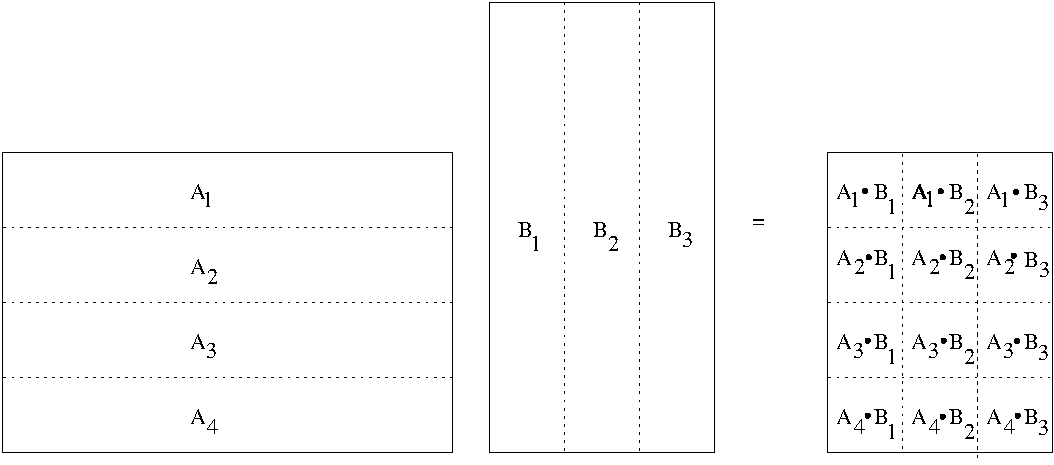
\includegraphics[height=1.5in]{4_matchop}}
\caption{Schematic of matrix multiplication as the inner product of 
rows and columns of the product matrices.
\label{fig_matchop}}
\end{figure}

It is {\em important} to notice that the matrix product $AB$ only
makes sense if the the number of columns of $A$ equals the number of
rows of $B$.  So $A^2=AA$ only makes sense for a square matrix.

Here is an example
\[
\left[\matrix{
1&0&1&2\cr
1&1&1&4\cr
0&0&1&1\cr
}\right]
\left[\matrix{
1&2\cr
3&4\cr
5&6\cr
7&8\cr
}\right]
=
\left[\matrix{
1\times 1+ 0\times 3+ 1\times 5+ 2\times 7& 1\times 2+ 0\times 4+ 1\times 6+ 2\times 8\cr
1\times 1+ 1\times 3+ 1\times 5+ 4\times 7& 1\times 2+ 1\times 4+ 1\times 6+ 4\times 8\cr
0\times 1+ 0\times 3+ 1\times 5+ 1\times 7& 0\times 2+ 0\times 4+ 1\times 6+ 1\times 8\cr
}\right] 
=
\left[\matrix{
20&24\cr
37&44\cr
12&14\cr
}\right]
\]

Notice that if 
$A$ is an $m\times n$ matrix, and
\[
\xx=
\left[\matrix{
x_1\cr
x_2\cr
x_3\cr
\vdots\cr
x_n\cr
}\right]
\]
and
\[
\bb=
\left[\matrix{
b_1\cr
b_2\cr
b_3\cr
\vdots\cr
b_m\cr
}\right]
\]
Then the equation 
\begin{equation}
\label{eq:matrixvector}
A\xx=\bb
\end{equation} 
is a short way of writing the system of linear equations corresponding
to the augmented matrix $[A|\bb]$. Further, it is seen that $A {\bf x}$ is a linear combination of the columns of $A$ with coefficients $\bf x$, that is 
\[
A {\bf x} = x_1 {\bf a}_1 + x_2 {\bf a}_2 + \cdots + x_n {\bf a}_n 
\]
where ${\bf a}_j$, $j=1 \cdots n$ are the {\em column vectors} of $A$, each of which have $m$ components. Thus, the linear system (\ref{eq:matrixvector}) is equivalent to the problem of writing $\bf b$ as a linear combination of the columns of $A$. The reader can look back at the discussion in section~\ref{s:geom} to see examples of this connection. 

We will see shortly why matrix multiplication is defined the way it
is. For now, you should be aware of some important properties that
{\it don't} hold for matrix multiplication, even though they are true
for multiplication of numbers. First of all, in general, $AB$ is {\it
not} equal to $BA$, even when both products are defined and have the
same size.  For example, if
\[
A=\left[\matrix{0&1\cr 0&0\cr}\right]
\]
and
\[
B=\left[\matrix{1&0\cr 0&0\cr}\right]
\]
then
\[
AB=\left[\matrix{0&0\cr 0&0\cr}\right]
\]
but
\[
BA=\left[\matrix{0&1\cr 0&0\cr}\right].
\]
This example also shows that two non-zero matrices can be multiplied
together to give the zero matrix.

Here is a list of properties that do hold for matrix multiplication.
\begin{enumerate}
\item $A+B=B+A$
\item $A+(B+C)=(A+B)+C$
\item $s(A+B)=sA+sB$
\item $(s+t)A=sA+tA$
\item $(st)A=s(tA)$
\item $1A=A$
\item $A+\zv=A$ (here $\zv$ is the matrix with all entries zero)
\item $A-A=A+(-1)A=\zv$
\item $A(B+C)=AB+AC$
\item $(A+B)C=AC+BC$
\item $A(BC)=(AB)C$
\item $s(AB)=(sA)B=A(sB)$
\end{enumerate}

\subsection{MATLAB}
\label{s_MAT_matmult}

Multiplication of matrices can be done using the {\tt *} operator 
just as for multiplication of scalars. An error results if the 
matrices are not of compatible size. Powers of matrices can be found 
using the \verb+^+ command like for scalars. The MATLAB command 
\begin{verbatim}
A^4 
\end{verbatim}
produces the same result as 
\begin{verbatim} 
A*A*A*A
\end{verbatim}
where {\tt A} is a previously defined, square matrix. Using these 
commands might be helpful in working out the details of Problem~\ref{op3_3}
below, although you should work out the first few matrix powers by hand 
for practise. Taking high powers of a matrix will also be helpful in 
understanding the long time behaviour of random walks described 
in Section~\ref{s_random}. 

\subsection{Problems}

\begin{problem}
\label{op3_1}
Define 
\[
A=\left[\matrix{
1&2&3\cr 1&2&1\cr
}\right]
B=\left[\matrix{
-1&2\cr -3&1\cr -2&1\cr
}\right]
C=\left[\matrix{
2&-2&0\cr
}\right]
D=\left[\matrix{
2\cr -11\cr 2\cr
}\right]
\]
Compute all products of two of these (i.e., $AB$, $AC$, etc.) that are
defined.
\end{problem}

\begin{problem}
\label{2009_a6_4}
Consider the following matrices:
\[ {\bf A}=
\left[
\begin{array}{c c}
3 & 0 \\ -1 & 2\\ 1 & 1
\end{array}
\right];
\hspace{4mm}
{\bf B}=\left[
\begin{array}{c c}
0 & 1\\ 0& 0
\end{array}
\right];\hspace{4mm}
{\bf C}=
\left[
\begin{array}{c c c}
1 & 4 & 2\\
3 & 1 & 5
\end{array}
\right].
\]
Compute all the possible products between them.
\end{problem}

\begin{problem}
\label{op3_2}
Compute $A^2=AA$ and $A^3=AAA$ for 
\[
A=\left[\matrix{
0&a&b\cr 0&0&c\cr 0&0&0\cr
}\right]
\]
and
\[
A=\left[\matrix{
1&0&a\cr
0&1&0\cr
0&0&1\cr
}\right]
\]
\end{problem}

\begin{problem}
\label{op3_3}
Let 
\[
A=\left[\matrix{
1&1\cr 0&1\cr
}\right]
\]
\begin{enumerate}[(a)]
\item Find $A^2$, $A^3$ and $A^4$.
\item Find $A^k$ for all positive integers $k$.
\item Find $e^{tA}$ (part of the problem is to invent a reasonable
definition!)
\item Find a square root of $A$ (i.e., a matrix $B$ with
$B^2=A$).
\item Find all square roots of $A$.  
\end{enumerate}
\end{problem}

\begin{problem}
\label{op3_4}
Compute $A^k$ for $k=2,3,4$ when
\[
A=\left[\matrix{
0&1&0&0\cr
0&0&1&0\cr
0&0&0&1\cr
0&0&0&0\cr
}\right]
\]
\end{problem}

\section{Linear Transformations and Matrices}

\subsection{Linear Transformations}

Recall that a function $f$ is a rule that takes an input value $x$ and
produces an output value $y=f(x)$. Functions are sometimes called
transformations or maps (since they transform, or map, the input value
to the output value).  In calculus, you have mostly dealt with
functions whose input values and output values are real
numbers. However, it is also useful to consider functions whose input
values and output values are vectors.

We have already encountered this idea when we discussed quadratic
functions. A quadratic function such as
$f(x_1,x_2,x_3)=x_1^2+x_2^2+x_3^2$ can be considered as a
transformation (or map) whose input is the vector $\xx=[x_1,x_2,x_3]$
and whose output is the number $y=x_1^2+x_2^2+x_3^2$.  In this case we
could write $f(x_1,x_2,x_3)$ as $f(\xx)$.

An example of a transformation whose inputs and outputs are both
vectors in two dimensions is rotation by some angle, say
$45^\circ$. If $\xx$ is the input vector, then the output vector
$R(\xx)$ is the vector you get by rotating $\xx$ by $45^\circ$ in the
counter-clockwise direction as shown in Figure~\ref{fig_2drot} (left). 

\begin{figure}
\centerline{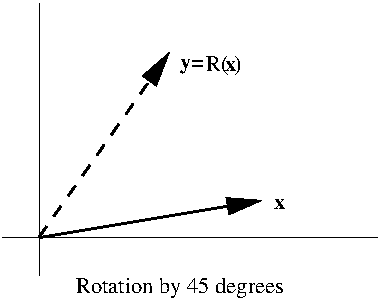
\includegraphics[height=1.5in]{4_2drot}
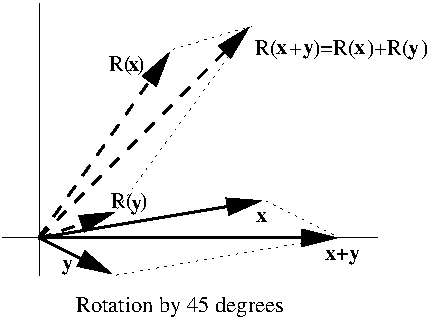
\includegraphics[height=1.5in]{4_rotlinear}}
\caption{Rotation of a vector in 2D (left), graphical evidence that
property (i) of linear transformations holds for rotation in 2D
(right).
\label{fig_2drot}}
\end{figure}

A transformation $T$ is called {\it linear} if for any two 
input vectors $\xx$ and $\yy$ and any two numbers $s$ and $t$, 
\begin{equation}
\label{eq_linear}
T(s\xx + t\yy) = s T(\xx) + t T(\yy)
\end{equation}
This condition is saying that when we scalar multiply and add two
vectors, it doesn't matter whether we (i) do scalar multiplication and
addition first and then apply a linear transformation, or (ii) do a
linear transformation first and then do scalar multiplication and
addition. In both cases we get the same answer.  The linearity
condition (\ref{eq_linear}) is equivalent to the following two conditions:
\begin{enumerate}[(i)]
\item For any two vectors $\xx$ and $\yy$,
\[
T(\xx + \yy) = T(\xx) + T(\yy).
\]
\item For any vector $\xx$ and any scalar $s$,
\[
T(s\xx) = sT(\xx)
\]
\end{enumerate}

Notice that the quadratic function $f$ above is not a linear transformation,
since 
\[
f(2\xx) = (2x_1)^2+(2x_2)^2+(2x_3)^2 = 4(x_1^2+x_2^2+x_3^2)=4f(\xx).
\]
So $f(2\xx)$ is not equal to $2f(\xx)$ as would need to be true if $f$
were linear.

However, rotation by $45^\circ$ is a linear transformation. The
picture in Figure~\ref{fig_2drot} (right) demonstrates that condition
(i) holds.

The most important example of a linear transformation is multiplication by a
matrix. If we regard vectors as column vectors, then multiplying an $n$
dimensional vector $\xx$ with an $m\times n$ matrix $A$ results in an $m$
dimensional vector $\yy=A\xx$. The linearity property (\ref{eq_linear}) is a
consequence of properties 9 and 12 of matrix multiplication listed in 
Section~\ref{s_matop}. We will see
that in fact every linear transformation is of this form.

\subsection{Rotations in two dimensions}

Let us obtain a formula for the transformation that rotates a vector
in two dimensions counterclockwise by $\theta$ degrees. Let $\xx$ be
an arbitrary vector. Denote by ${\rm Rot}_\theta\xx$ the vector
obtained by rotating $\xx$ counterclockwise by $\theta$ degrees.  If
the angle between $\xx$ and the $x$ axis is $\phi$, then the
components of $\xx$ can be written $\xx=[x_1,x_2]$ with
$x_1=\|x\|\cos(\phi)$ and $x_2= \|x\|\sin(\phi)$. This is shown
graphically in Figure~\ref{fig_proj1} (right). To obtain the vector
that has been rotated by $\theta$ degrees, we simply need to add
$\theta$ to $\phi$ in this representation. Thus $\yy={\rm Rot}_\theta
\xx = [y_1,y_2]$, where $y_1 = \|x\|\cos(\phi+\theta)$ and $y_2=
\|x\|\sin(\phi+\theta)$.

\begin{figure}
\label{fig_proj1}
\centerline{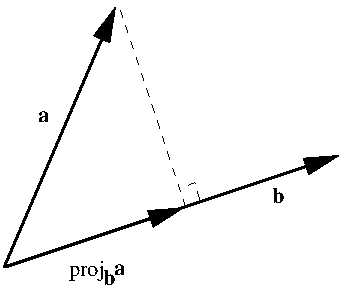
\includegraphics[height=1.5in]{4_proj}
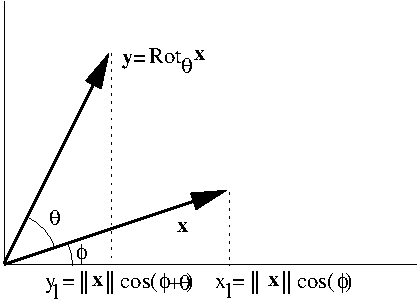
\includegraphics[height=1.5in]{4_rotang}}
\caption{Graphical representation of a projection (left). Details of
components in a rotation by an angle $\theta$.}
\end{figure}

To simplify this we can use the addition formulae for sin and cos. Recall that
\begin{eqnarray*}
\cos(a+b)&=&\cos(a)\cos(b)-\sin(a)\sin(b) \\
\sin(a+b)&=&\cos(a)\sin(b)+\sin(a)\cos(b)
\end{eqnarray*}
Thus 
\begin{eqnarray*}
y_1 &= &\|x\|\cos(\phi+\theta) \\
&=&\|x\|(\cos(\phi)\cos(\theta)-\sin(\phi)\sin(\theta)) \\
&=&\cos(\theta)x_1-\sin(\theta)x_2
\end{eqnarray*}
and so 
\begin{eqnarray*}
y_2 &=& \|x\|\sin(\phi+\theta) \\
&=&\|x\|(\sin(\phi)\cos(\theta)+\cos(\phi)\sin(\theta)) \\
&=&\sin(\theta)x_1+\cos(\theta)x_2 
\end{eqnarray*}
Notice now that this can be written as a matrix product:
\[
\left[\matrix{y_1\cr y_2\cr}\right]
=\left[\matrix{\cos(\theta)&-\sin(\theta)\cr \sin(\theta)&\cos(\theta)}\right]
\left[\matrix{x_1\cr x_2\cr}\right]
\]
The matrix 
\[
\left[\matrix{\cos(\theta)&-\sin(\theta)\cr
\sin(\theta)&\cos(\theta)}\right],
\]
also denoted ${\rm Rot}_\theta$, is called a rotation matrix. What
this formula is saying is that the linear transformation of rotation
by $\theta$ degrees in the same as the linear transformation of
multiplication by the matrix. In other words, if we want to know the
co-ordinates of the vector obtained by rotating $\xx$ by $\theta$
degrees, we simply calculate ${\rm Rot}_\theta\xx$.

\subsection{Projections in two dimensions}

Now we consider the transformation which projects a vector $\xx$ in
the direction of another vector $\aa$ as shown in Figure~\ref{fig_proj1}
(left). We already have a formula for this transformation. In the
{\em special case} that $\aa$ has unit length, the formula is
\[
{\rm Proj}_\aa \xx = (\xx\cdot\aa)\aa.
\]
It follows from the properties of the dot product that 
\begin{eqnarray*}
{\rm Proj}_\aa (s\xx +t\yy) &=& ((s\xx +t\yy)\cdot\aa)\aa \\
&=& ((s\xx\cdot\aa +t\yy\cdot\aa)\aa \\
&=& s((\xx\cdot\aa)\aa) + t((\yy\cdot\aa)\aa) \\
&=& s{\rm Proj}_\aa \xx + t {\rm Proj}_\aa \yy
\end{eqnarray*}
Thus ${\rm Proj}_\aa$ is a linear transformation. Let us now see that 
${\rm Proj}_\aa$ is also given by multiplication by a matrix. If 
$\aa=[a_1,a_2]$ (still considered to be a {\em unit vector}), then 
\begin{eqnarray}
\nonumber
{\rm Proj}_\aa \xx &=&
\left[\matrix{(x_1a_1+x_2a_2)a_1\cr(x_1a_1+x_2a_2)a_2\cr}\right] \\
\nonumber 
&=&\left[\matrix{a_1^2x_1+a_1a_2x_2\cr a_2a_1x_1+a_2^2x_2\cr}\right] \\
\label{eq:proj2d}
&=&\left[\matrix{a_1^2&a_1a_2\cr a_2a_1&a_2^2\cr}\right]\left[\matrix{x_1\cr
x_2\cr}\right]
\end{eqnarray}
If $\aa$ is the unit vector making an angle of $\theta$ with the $x$ axis,
then $a_1=\cos(\theta)$ and $a_2=\sin(\theta)$. Using half angle formulae,
we have
\begin{eqnarray*}
a_1^2 &=& \cos^2(\theta)={{1+\cos(2\theta)}\over{2}} \\
a_2^2 &=& \sin^2(\theta)={{1-\cos(2\theta)}\over{2}} \\
a_1a_2 &=& \cos(\theta)\sin(\theta)={{\sin(2\theta)}\over{2}}
\end{eqnarray*}
Thus the matrix which when multiplied by $\xx$ produces the projection
of $\xx$ onto the line making an angle of $\theta$ with the $x$ axis
is given by
\[
{\rm Proj}_\theta = 
{{1}\over{2}}\left[\matrix{1+\cos(2\theta)&\sin(2\theta)\cr 
\sin(2\theta)&1-\cos(2\theta)\cr}\right]
\]

Note that if $\bf a$ is nonzero but {\em not a unit vector}, then the unit vector 
\[
\hat{\bf a} = \frac{{\bf a}}{\| {\bf a} \|} = \frac{(a_1, a_2)}{\sqrt{a_1^2 +a_2^2}} 
\]
points in the same direction as $\bf a$ and so (\ref{eq:proj2d}) becomes 
\[
{\rm Proj}_\aa = \left[\matrix{a_1^2/(a_1^2 + a_2^2) &a_1a_2/(a_1^2 + a_2^2)\cr
 a_2a_1/(a_1^2 + a_2^2) & a_2^2/(a_1^2 + a_2^2)\cr}\right]
\]

\subsection{Reflections in two dimensions}

A third example of a geometric linear transformation is reflection
across a line. The following figure illustrates reflection across a
line making an angle $\theta$ with the $x$ axis. Let ${\rm Ref}_\theta
\xx$ denote the reflected vector as shown in Figure~\ref{fig_reflect}.

\begin{figure}
\centerline{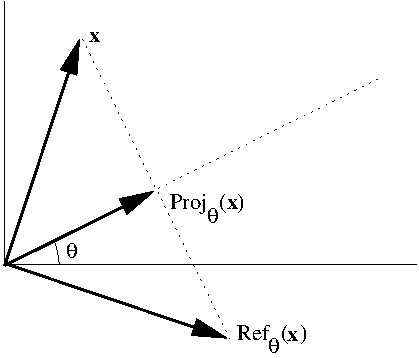
\includegraphics[height=1.5in]{4_reflect}}
\caption{Graphical representation of a reflection.
\label{fig_reflect}}
\end{figure}

We can obtain the matrix for reflection from the following observation.
The vector with tail at $\xx$ and head at ${\rm Proj}_\theta \xx$ is 
${\rm Proj}_\theta \xx - \xx$. If we add twice this vector to $\xx$, 
we arrive at ${\rm Ref}_\theta \xx$. Therefore
\begin{eqnarray*}
{\rm Ref}_\theta \xx &=& \xx + 2({\rm Proj}_\theta \xx - \xx) \\
&=& 2{\rm Proj}_\theta \xx - \xx
\end{eqnarray*}
Now if $I=\left[\matrix{1&0\cr 0&1\cr}\right]$, then $I\xx = \xx$ for any 
vector $\xx$, since
\[
\left[\matrix{1&0\cr 0&1\cr}\right]\left[\matrix{x_1\cr x_2\cr}\right]
=\left[\matrix{1x_1+0x_2\cr 0x_1+1x_2\cr}\right]
=\left[\matrix{x_1\cr x_2\cr}\right]
\]
$I$ is called the identity matrix.

Now we can write
\[
{\rm Ref}_\theta \xx= 2{\rm Proj}_\theta \xx - I\xx
=(2{\rm Proj}_\theta - I)\xx.
\]
This means that the matrix for reflections is $2{\rm Proj}_\theta - I$. 
Explicitly
\begin{eqnarray*}
{\rm Ref}_\theta&=&\left[\matrix{1+\cos(2\theta)&\sin(2\theta)\cr 
\sin(2\theta)&1-\cos(2\theta)\cr}\right]-\left[\matrix{1&0\cr 0&1\cr}\right] \\
&=&\left[\matrix{\cos(2\theta)&\sin(2\theta)\cr
\sin(2\theta)&-\cos(2\theta)\cr}\right]
\end{eqnarray*}

\subsection{Every linear transformation is multiplication by a matrix}

We have just seen three examples of linear transformations whose
action on a vector is given by multiplication by a matrix. Now we will
see that for {\em any} linear transformation $T(\xx)$ there is a
matrix $T$ such that $T(\xx)$ is the matrix product $T\xx$.

To illustrate this suppose that $T$ is a linear transformation that takes
three dimensional vectors as input.

Let $\eee_1$, $\eee_2$ and $\eee_3$ be the standard basis vectors in three
dimensions, that is
\[
\eee_1 = \left[\matrix{1\cr 0\cr 0\cr}\right]
\eee_2 = \left[\matrix{0\cr 1\cr 0\cr}\right]
\eee_3 = \left[\matrix{0\cr 0\cr 1\cr}\right]
\]
Then any vector can be written
\[
\xx = \left[\matrix{x_1\cr x_2\cr x_3\cr}\right]
=x_1\left[\matrix{1\cr 0\cr 0\cr}\right]
+x_2\left[\matrix{0\cr 1\cr 0\cr}\right]
+x_3\left[\matrix{0\cr 0\cr 1\cr}\right]
=x_1\eee_1+x_2\eee_2+x_3\eee_3
\]
Now, using the linearity property of the linear transformation
$T$, we obtain
\[
T(\xx)=T(x_1\eee_1+x_2\eee_2+x_3\eee_3)=x_1T(\eee_1)+x_2T(\eee_2)+x_3T(\eee_3)
\]
Now take the three vectors $T(\eee_1)$, $T(\eee_2)$ and $T(\eee_3)$
and put them in the columns of a matrix which we'll also call $T$. Then
\[
T\xx = \Bigg[T(\eee_1)\Bigg|T(\eee_2)\Bigg|T(\eee_3)\Bigg]
\left[\matrix{x_1\cr x_2\cr x_3\cr}\right]
=T(\eee_1)x_1+T(\eee_2)x_2+T(\eee_3)x_3  = T(\xx)
\]
In other words, the action of the transformation $T$ on a vector $\xx$
is the same as multiplying $x$ by the matrix 
$T=\Bigg[T(\eee_1)\Bigg|T(\eee_2)\Bigg|T(\eee_3)\Bigg]$

The same idea works in any dimension.  To find the matrix of a linear
transformation $T(\xx)$ we take the standard basis vectors $\eee_1,
\eee_2,\ldots, \eee_n$ (where $\eee_k$ has zeros everywhere except for
a $1$ in the $k$th spot) and calculate the action of the linear
transformation on each one. We then take the transformed vectors
$T(\eee_1), T(\eee_2),\ldots, T_(\eee_n)$ and put them into the
columns of a matrix
$T=\Bigg[T(\eee_1)\Bigg|T(\eee_2)\Bigg|\cdots\Bigg|T(\eee_n)\Bigg]$.
This matrix $T$ then reproduces the action of the linear
transformation, that is, $T(\xx)=T\xx$.

To see how this works in practise, let's recalculate the matrix for rotations
in two dimensions. Under a rotation angle of $\theta$, the vector $\eee_1=
\left[\matrix{1\cr 0\cr}\right]$ gets transformed to 
$T(\eee_1)=\left[\matrix{\cos(\theta)\cr \sin(\theta)\cr}\right]$ while 
the vector $\eee_2=
\left[\matrix{0\cr 1\cr}\right]$ gets transformed to 
$T(\eee_2)=\left[\matrix{-\sin(\theta)\cr
\cos(\theta)\cr}\right]$. This is shown graphically in
Figure~\ref{fig_erot}. 

\begin{figure}
\centerline{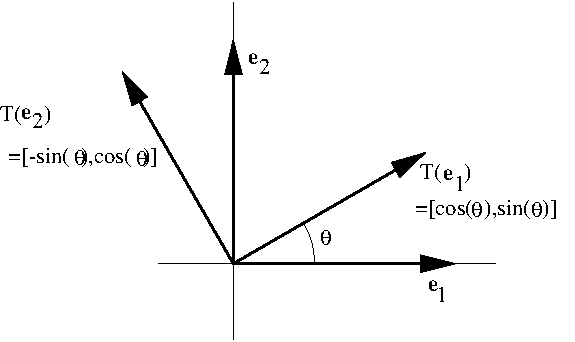
\includegraphics[height=1.5in]{4_erot}}
\caption{Derivation of the matrix representing 2D rotation by rotating
coordinate directions. 
\label{fig_erot}}
\end{figure}

According to our prescription, we must now put these two vectors into the 
columns of a matrix. This gives the matrix
\[
T=\left[\matrix{\cos(\theta)&-\sin(\theta)\cr
\sin(\theta)&\cos(\theta)\cr}\right]
\]
which is exactly the same as ${\rm Rot}_\theta$.

\subsection{Composition of linear transformations and matrix product}

Suppose we apply one linear transformation $T$ and then follow it by another
linear transformation $S$. For example, think of first rotating a vector and
then reflecting it across a line.  Then $S(T(\xx))$ is again a linear
transformation, since
\[
S(T(s\xx + t\yy))= S(sT(\xx)+tT(\yy))= sS(T(\xx)) + tS(T(\yy)).
\]
What is the matrix for the composition $S(T(\xx))$? We know that there
are matrices $S$ and $T$ that reproduce the action of $S(\xx)$ and
$T(\xx)$.  So $T(\xx)$ is the matrix product $T\xx$ and $S(T\xx))$ is
the matrix product $S(T\xx)$ (here the parenthesis just indicate in
which order we are doing the matrix product) But matrix multiplication
is associative. So $S(T\xx)=(ST)\xx$. In other words the matrix for
the composition of $S(\xx)$ and $T(\xx)$ is simply the matrix product
of the corresponding matrices $S$ and $T$.

For example, to compute the matrix for the transformation of rotation by
$45^\circ$ followed by reflection about the line making an angle of $30^\circ$
with the $x$ axis we simply compute the product
\begin{eqnarray*}
{\rm Ref}_{30^\circ}{\rm Rot}_{45^\circ}
&=&\left[\matrix{\cos(60^\circ)&\sin(60^\circ) \cr
\sin(60^\circ)&-\cos(60^\circ)\cr}\right]
\left[\matrix{\cos(45^\circ)&-\sin(45^\circ)\cr
\sin(45^\circ)&\cos(45^\circ)}\right] \\
&=&\left[\matrix{{{1}\over{2}}&{{\sqrt{3}}\over{2}}\cr
{{\sqrt{3}}\over{2}}&-{{1}\over{2}}\cr}\right]
\left[\matrix{{{\sqrt{2}}\over{2}}&-{{\sqrt{2}}\over{2}}\cr
{{\sqrt{2}}\over{2}}&{{\sqrt{2}}\over{2}}}\right] \\
&=&\left[\matrix{{{\sqrt{2}+\sqrt{6}}\over{4}}&{{-\sqrt{2}+\sqrt{6}}\over{4}}\cr
{{\sqrt{6}-\sqrt{2}}\over{4}}&{{-\sqrt{6}-\sqrt{2}}\over{4}}\cr}\right]
\end{eqnarray*}

\subsection{Problems}

\begin{problem}
\label{op3_5}
Let $\aa$ be a fixed nonzero vector. Show that the transformation $T(\xx)=\xx+\aa$
is not a linear transformation.
\end{problem}

\begin{problem}
\label{op3_6}
Let $\aa$ be a fixed vector. Show that the transformation $T(\xx)=\aa\cdot\xx$
is a linear transformation (whose output values are numbers).
\end{problem}

\begin{problem}
\label{op3_7}
Find the matrices which project on the lines
\begin{enumerate}[(a)]
\item $x_1=x_2$ 
\item $3x_1+4x_2=0$
\end{enumerate}
\end{problem}

\begin{problem}
\label{op3_8}
Find the matrices that reflect about the lines
\begin{enumerate}[(a)]
\item $x_1=x_2$ 
\item $3x_1+4x_2=0$
\end{enumerate}
\end{problem}

\begin{problem}
\label{op3_9}
Find the matrices which rotate about the origin in two dimensions by
\begin{enumerate}[(a)]
\item $\pi/4$
\item $\pi/2$ 
\item $\pi$
\end{enumerate}
\end{problem}

\begin{problem}
\label{op3_11}
Find the matrix which first reflects about the line making an angle of $\phi$
with the $x$ axis, and then reflects about the line making an angle of $\theta$
with the $x$ axis. Give another geometric interpretation of this matrix.
\end{problem}

\begin{problem}
\label{2009_a7_2}
Let $f:\mathbb{R}^2\to \mathbb{R}^2$ be the linear transformation  that  reflects points across the line $x=2y$.
    \begin{enumerate}
        \item What is the image of $(1,10)$, that is, the vector
\[
f \left(\left[ \begin{array}{c}
1 \\ 10
\end{array} \right]\right)?
\]
        \item Write down the matrix of $f$.\\
    \end{enumerate}
\end{problem}

\begin{problem}
\label{2009_a7_3}
Let $g:\mathbb{R}^2\to \mathbb{R}^2$ be the linear transformation
that first reflects points across the line $x=-y$ and then rotates points $\pi/2$ radians.     Write down the matrix of $f$.
\end{problem}

\begin{problem}
\label{op3_12}
Find the matrix that rotates about the $z$ axis by and angle of $\theta$ in 
three dimensions.
\end{problem}

\begin{problem}
\label{2009_a6_5}
Let $T:\mathbb R^4\to \mathbb R^3$ be the map defined by
%
$$T(x_1,x_2,x_3,x_4)=(x_1+4x_2+5x_3,3x_1-2x_2+x_3-x_4,-x_1-x_3+x_4)$$
%
Show that $T$ is a linear transformation.
\end{problem}

\begin{problem}
\label{2009_a7_1}
Let $T:\mathbb{R}^2\to \mathbb{R}^3$ given by $T({\bf x})=A\mathbf{x}$,
where $$A=\left[\begin{array}{c c}1 & 2\\ 0 & 1\\ 1 & 1\end{array}\right].$$
Determine whether each given vector is in the range of $T$. Recall that the
range of $T$ is every vector that can ``come out" or $T$, that is every
vector in $\mathbb{R}^3$ that can be written as $T({\bf x})$ for some
$\bf x$ in $\mathbb{R}^2$. Note that answering these questions is the
same as determining if a linear system has a solution.
\begin{enumerate}
\item $\left[\begin{array}{c}1\\ 4\\ 2 \end{array}\right].$
\item $\left[\begin{array}{c}1\\ 1\\ 1 \end{array}\right].$
\end{enumerate}
\end{problem}

\begin{problem}
\label{2009_a7_4}
Suppose $T:\mathbb{R}^3\to \mathbb{R}^2$ is a linear transformation
such that
$$
T\left(\left[\begin{array}{c}1\\ 0\\ 0 \end{array}\right]\right)=\left[\begin{array}{c}1\\ 1\end{array}\right],\quad
T\left(\left[\begin{array}{c}1\\ -1\\ 0 \end{array}\right]\right)=\left[\begin{array}{c}2\\ 0\end{array}\right],\quad
T\left(\left[\begin{array}{c}0\\0 \\ 1 \end{array}\right]\right)=\left[\begin{array}{c}-1\\ 5\end{array}\right].
$$
    \begin{enumerate}
        \item Find  $T\left(\left[\begin{array}{c}1\\ 2\\ 3 \end{array}\right]\right)$.
        \item Write down the matrix of $T$.
    \end{enumerate}
\end{problem}

\begin{problem}
\label{2009_a7_5}
Let $g:\mathbb{R}^3\to \mathbb{R}^2$ and $h:\mathbb{R}^2\to \mathbb{R}^4$ be linear transformations given by
% \begin{align*}
$$
g\left(\left[\begin{array}{c}x_1\\ x_2\\ x_3 \end{array}\right]\right)=\left[\begin{array}{c}x_1-x_3+x_2\\ x_3-2x_2\end{array}\right],\quad
h\left(\left[\begin{array}{c}x_1\\ x_2 \end{array}\right]\right)=\left[\begin{array}{c}x_1\\ -x_1\\x_2\\ -x_2\end{array}\right].
$$
% \end{align*}
The questions below concern $h \circ g$, the composition of $h$ and $g$ defined
by
$$
h \circ g ({\bf x}) = h(g({\bf x}))
$$
for ${\bf x} \in \mathbb{R}^3$. Note that this composition is defined because
the output of $g$ and the input of $h$ have the same dimension, two.
    \begin{enumerate}
     \item Find $h \circ g\left(\left[\begin{array}{c}1\\0\\ -5 \end{array}\right]\right)$.
     \item Find  the matrices of $g$ and $h$.
     \item Find the matrix of $h \circ g$.
    \end{enumerate}
\end{problem}

\section{Application: random walks}
\label{s_random}

Consider a system with three states, labelled $1$, $2$ and $3$ in 
Figure~\ref{fig_markov}.

\begin{figure}
\centerline{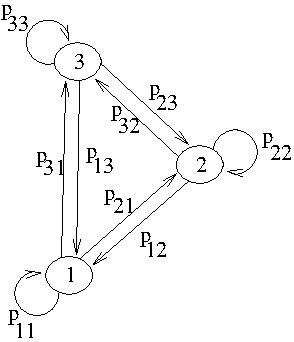
\includegraphics[height=1.5in]{4_markov}}
\caption{Graphical description of a random walk with three states.
\label{fig_markov}}
\end{figure}

To make the problem more vivid, one can imagine these as being actual
locations. A random walker starts off at some location, say location
$1$ at time $0$.  Then at a sequence of times, $1,2,\ldots,n\ldots$,
the walker either stays where he is, or moves to one of the other
locations. The next location is chosen randomly, but according to the
transition probabilities $p_{i,j}$.  These are numbers between $0$ and
$1$ that measure how likely it is that, starting from location $j$,
the walker will move to location $i$.  If $p_{i,j}=0$, then there is
no chance that the walker will move from $j$ to $i$, and if
$p_{i,j}=1$, then the walker will move for sure from $j$ to $i$.

Since the walker must either move from $j$ to another site or stay put, 
the sum of these probabilities must equal one:
\[
p_{1,j}+p_{2,j}+p_{3,j}=\sum_{i=1}^3p_{i,j}=1
\]
At each time $n$ there is a vector 
\[
\xx_n=\left[\matrix{x_{n,1}\cr x_{n,2}\cr x_{n,3}\cr}\right]
\]
that gives the probabilities that the walker is in location $1$, $2$
or $3$ at time $n$. Let us compute the vector $\xx_{n+1}$, given
$\xx_n$. To start, we must compute $x_{n+1,1}$, the probability that
the walker is at location $1$ at time $n+1$. There are three ways the
walker can end up at location $1$. The walker might have been at
location $1$ at time $n$ and have stayed there. The probability of
this is $p_{1,1}x_{n,1}$. Or he might have been at location $2$ and
have moved to $1$. The probability of this is
$p_{1,2}x_{n,2}$. Finally, he might have been at location $3$ and have
moved to $1$. The probability of this is $p_{1,3}x_{n,3}$. Thus the
total probability that the walker is at location $1$ at time $n+1$ is
the sum
\[
x_{n+1,1} = p_{1,1}x_{n,1} + p_{1,2}x_{n,2} + p_{1,3}x_{n,3}
\]
Similarly, for all $i$
\[
x_{n+1,i} = p_{i,1}x_{n,1} + p_{i,2}x_{n,2} + p_{i,3}x_{n,3}
\]
But this is exactly the formula for matrix multiplication. So
\[
\xx_{n+1}= P\xx_n
\]
where $P$ is the matrix with entries $[p_{ij}]$.

Now suppose the initial probabilities are given by some vector $\xx_0$. For
example, if the walker starts off at location $1$, then
\[
\xx_0=\left[\matrix{1\cr 0\cr 0\cr}\right]
\]
Then after one time step, we have
\[
\xx_1= P\xx_0
\]
Then,
\[
\xx_2=P\xx_1=P^2\xx_0
\]
and so on, so after $n$ time steps
\[
\xx_n=P^n\xx_0
\]

Notice that the sum $x_{n,1}+x_{n,2}+x_{n,3}=\sum_{i=1}^3x_{n,i}$
should equal one, since the total probability of being in one of the
three locations must add up to one.

If the initial vector has this property, then it is preserved for all
later times.  To see this, suppose that $\sum_{j=1}^3x_j=1$ Then,
since $\sum_{i=1}^3p_{ij}=1$
\begin{eqnarray*}
\sum_{i=1}^3 (Px)_i &=&\sum_{i=1}^3 \sum_{j=1}^3 p_{ij}x_j \\
&=&\sum_{j=1}^3\left(\sum_{i=1}^3p_{ij}\right)x_j \\
&=&\sum_{j=1}^3x_j \mbox{\ = \ } 1
\end{eqnarray*}
In other words, the vector for the next time step also has components
summing to one.  Of course, one can generalize this to a system with
an arbitrary number of states or locations. Later in the course we
will see how to use eigenvalues and eigenvectors to efficiently
compute the limit as $n$ tends to infinity of this expression.

A specific but somewhat nerdy example is given below. 
\begin{example}
\label{ex_sorceror1}
Ydnew the sorcerer and his apprentice, Xavier, have a magical duel as 
part of a circus act. They take turns casting spells, which don't 
always work, but when they do the opponent is knocked out. Xavier always 
goes first in the duel but his spells only work 1/3 of the time. 
Ydnew's spells work 1/2 of the time. When they practise, they find that 
each wins half the time. However, in performances, the duel is limited 
to three attempts by Xavier. After that, if there has been no knock-out, 
Ydnew is declared the winner. 
\begin{enumerate}[(a)]
\item Describe the duel as a random walk. 
\item Write the matrix for the random walk. 
\item Use the matrix to analyze the probability that Ydnew will win 
the duel when Xavier's attempts are limited and also when they are 
unlimited. 
\end{enumerate}
{\rm There are four possible states:
\begin{enumerate}[(1)]
\item No winner yet, Xavier's turn
\item No winner yet, Ydnew's turn
\item Xavier has won.
\item Ydnew has won.
\end{enumerate}
These are shown with transition probabilities in 
Figure~\ref{fig_sorceror1}. The transition matrix with the node ordering 
we have chosen is 
\[
P = \left[ \begin{array}{cccc} 
0 & 1/2 & 0 & 0 \\
2/3 & 0 & 0 & 0 \\
1/3 & 0 & 1 & 0 \\
0 & 1/2 & 0 & 1 
\end{array} \right]
\]
The duel begins in state (1), that is Xavier's turn, no winner yet:
\[
\xx^{(0)} = \left[ \begin{array}{c} 1 \\ 0 \\ 0 \\ 0 \end{array}
   \right]
\]
The circus duel ends after 3 attempts by Xavier, that is after 5 
transitions in the state diagram (five rounds XYXYX). 
Using MATLAB we compute 
\[
\xx^{(5)} = P^5 \xx^{(0)} \approx \left[ \begin{array}{c} 0 \\ 0.0741 \\ 
   0.4815 \\ 0.4444 \end{array} \right].
\]
This means that Ydnew will win with probability 0.5185, the sum of the 
second and fourth components in $\xx^{(5)}$ (he can win by a knock-out 
or if Xavier has not defeated him after his third attempt). To 
investigate what happens in the unlimited turn version of the duel they 
use when they practise, you can compute 
\[
\xx^{(n)} = P^n \xx^{(0)}
\]
for $n$ increasingly large. This gives strong {\em numerical evidence} that 
\[
\lim_{n \rightarrow \infty} \xx^{(n)} = \left[ \begin{array}{c} 0 \\ 0 \\ 
1/2 \\ 1/2 \end{array} \right].
\]
That is, in the unlimited duel they each win half the time, as they 
observed. This unlimited case can be analyzed rigorously. The techniques 
used are not part of the course, but it is done below for completeness. 
Xavier has a chance to win on any odd turn. On turn 1 he can win if his 
spell works (1/3 chance). On turn 3 Xavier can win if his spell missed 
on turn 1, Ydnew missed on turn 2 but Xavier succeeds on turn 3 
($\frac{2}{3} \frac{1}{2} \frac{1}{3} = \frac{1}{9}$ chance). On turn 
5 he can win if there were failures in turns 1-4 but success on turn 5, 
with a chance of $\frac{2}{3} \frac{1}{2} \frac{2}{3} \frac{1}{2}
\frac{1}{3} = \frac{1}{27}$. Notice the pattern that each successive 
chance to win goes down by a factor of 3. The total chance of success 
is the sum of the chances to win at every opportunity:
\[
\frac{1}{3} + \frac{1}{9} + \frac{1}{27} + \cdots 
 = \frac{1}{3} (1 + \frac{1}{3} + \frac{1}{9} + \cdots )
 = \frac{1}{3} \sum_{i=0}^\infty \left( \frac{1}{3} \right)^i = 
   \frac{1}{3} \frac{1}{1-1/3} = \frac{1}{2} 
\]
as predicted from the MATLAB numerical results. To get the second last 
term above, the expression for the sum of a geometric series was used. 
}
\end{example}

\begin{figure}
\centerline{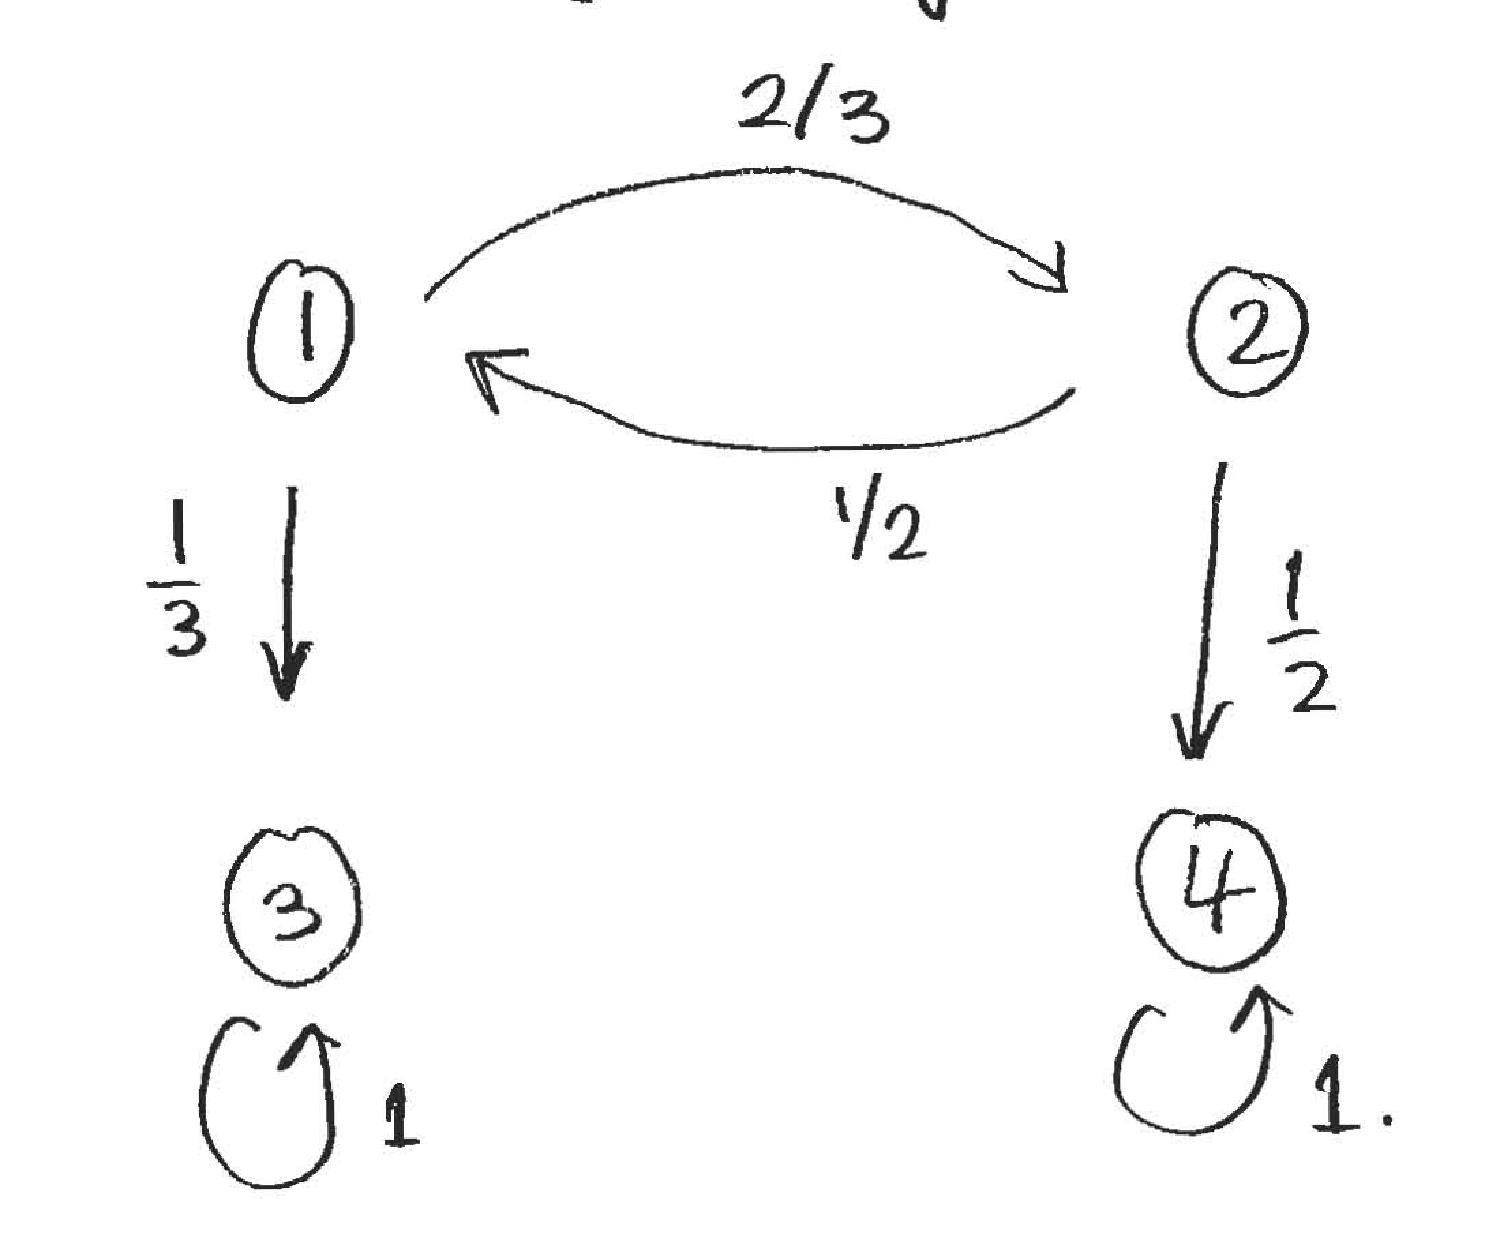
\includegraphics[height=1.5in]{4_sorceror1}}
\caption{Diagram of the sorcerers' duel described in 
Example~\ref{ex_sorceror1}.
\label{fig_sorceror1}}
\end{figure}

\begin{example}
\label{ex_sorceror2}
Investigate a modified sorcerer's duel to the one described in 
Example~\ref{ex_sorceror1} in which both sorcerers are given a shield 
which can protect them from one successful spell cast on them. 
{\rm Here, there are 10 possible states 
\begin{description}
\item[(1)] No winner yet, Xavier's turn, both have shields still.
\item[(2)] No winner yet, Xavier's turn, Xavier has lost his shield, 
but Ydnew still has his. 
\item[(3)] No winner yet, Xavier's turn, Xavier still has his shield, 
but Ydnew has lost his. 
\item[(4)] No winner yet, Xavier's turn, both have lost their shields. 
\item[(5-8)] Same as (1)-(4) above, but Ydnew's turn. 
\item[(9)] Xavier has won. 
\item[(10)] Ydnew has won. 
\end{description}
Using the ordering of states above, the transition matrix is 
\[
P = \left[
\begin{array}{cccccccccc}
 0 & 0 & 0 & 0 &1/2& 0 & 0 & 0 & 0 & 0 \\
 0 & 0 & 0 & 0 &1/2&1/2& 0 & 0 & 0 & 0 \\
 0 & 0 & 0 & 0 & 0 & 0 &1/2&1/2& 0 & 0 \\
 0 & 0 & 0 & 0 & 0 & 0 & 1/2 & 0 & 0 & 0 \\
2/3& 0 & 0 & 0 & 0 & 0 & 0 & 0 & 0 & 0 \\
 0 &2/3& 0 & 0 & 0 & 0 & 0 & 0 & 0 & 0 \\
1/3 & 0 &2/3& 0 & 0 & 0 & 0 & 0 & 0 & 0 \\
0 & 1/3  & 0 &2/3& 0 & 0 & 0 & 0 & 0 & 0 \\
 0 & 0 &1/3&1/3& 0 & 0 & 0 & 0 & 1 & 0 \\
 0 & 0 & 0 & 0 & 0 &1/2& 0 & 1/2 & 0 & 1 
\end{array} 
\right]
\]
This matrix can be entered in MATLAB (remember the techniques for entering 
sparse matrices, that is matrices with mostly zero entries, learnt in 
your computer lab \#2). Starting with $\xx^{(0)} = \eee_1$ we can compute
\[
\xx^{(5)} = P^5 \xx^{(0)} 
\]
numerically in MATLAB. Adding components 5-8 (Ydnew wins by default) and 
component 10 (Ydnew wins by knock-out) gives approximately 0.7778, the 
chance that Ydnew will win the circus duel. The unlimited duel can 
be investigated numerically, giving 
\[
\lim_{n \rightarrow \infty} P^n \xx^{(0)} \approx 
\left[ \begin{array}{c} 
0 \\ 0 \\ 0 \\ 0 \\ 0 \\ 0 \\ 0 \\ 0 \\ 0.3750 \\ 0.6250 
\end{array}
\right]
\]
So in an unlimited match, Ydnew will win about 62.5\% of the time. 
}
\end{example}

\subsection{Problems}

\begin{problem}
\label{op3_13}
Consider a random walk with $3$ states, where the probability of
staying in the same location is zero. Suppose
\begin{itemize}
\item the probability of moving from location $1$ to location $2$ is $1/2$
\item the probability of moving from location $2$ to location $1$ is $1/3$
\item the probability of moving from location $3$ to location $1$ is
$1/4$
\end{itemize}
Write down the matrix $P$. What is the probability that a walker
starting in location $1$ is in location $2$ after two time steps?
\end{problem}

\begin{problem}
\label{2009_a8_3}
Consider a random walk with 3 states, where the probability of
staying in the same location is zero. Suppose
\begin{itemize}
\item the probability of moving from location 1 to location 2 is 1/3, that is $p_{2,1}=\frac{1}{3}$.
\item the probability of moving from location 2 to location 1 is 2/5, that is $p_{1,2}=\frac{2}{5}$.
\item the probability of moving from location 3 to location 1 is 1/4, that is $p_{1,3}=\frac{1}{4}$.
\end{itemize}
\begin{enumerate}
\item Write down the matrix P.
\item What is the probability that a walker starting in
location 1 is in location 2 after three time steps?
\item What is the probability that a walker starting in
location 3 is in location 1 after two time steps?
\end{enumerate}
\end{problem}

\begin{problem}
\label{2009_a8_4}
Consider a random walk with 4 states, where all the probabilities
$p_{i,j}$ are equal to 1/4.
\begin{enumerate}
\item Compute $P$ and $P^n$, for every positive integer $n$.
\item Compute the probability location vectors $\mathbf{x}_n$ ($\mathbf{x}_n=P^n\mathbf{x}_0$)  in each of the following cases:
$$
\mathbf{x}_0=\left[\begin{array}{c}1\\0\\0\\0 \end{array}\right], \quad \mathrm{or} \quad
\mathbf{x}_0=\left[\begin{array}{c}0\\0\\0\\1\end{array}\right].
$$
\end{enumerate}
\end{problem}

\begin{problem}
\label{2009_a8_5}
Suppose that the matrix $P$ given below is the matrix of a random walk:
 $$
P=\left[\begin{array}{ccc}\frac{1}{3}& \frac{1}{4} & \frac{2}{5}\\ 0& \frac{1}{2}& \frac{1}{5}\\ \frac{2}{3}& \frac{1}{4}& \frac{2}{5} \end{array}\right].
$$
\begin{enumerate}
\item What is the probability that a walker starting in
location 2 is in location 1 after one time step?
\item What is the probability that a walker starting in
location 2 is in location 1 after two time steps?
\item If $\mathbf{x}_0=\left[\begin{array}{c}1/3\\1/3\\2/3 \end{array}\right]$
what is the probability that the walker is in location 3 after
two time steps?
\end{enumerate}
\end{problem}

\begin{problem}
\label{op3_14}
Consider a random walk with $3$ states, where all the probabilities
$p_{i,j}$ are all equal to $1/3$. What is $P$, $P^n$? Compute the
probabilities $P^n\xx_0$ when $\xx_0=\left[\matrix{1\cr 0\cr
0\cr}\right]$ ({em i.e} the walker starts in location $1$),
$\xx_0=\left[\matrix{0\cr 1\cr 0\cr}\right]$ ({em i.e.} the walker starts in
location $2$), and $\xx_0=\left[\matrix{0\cr 0\cr 1\cr}\right]$ ({em i.e.}
the walker starts in location $3$) 
\end{problem}

\begin{problem}
\label{newp4_1}
Consider a random walk with three states with transition probabilities 
shown in Figure~\ref{fig_newp4_1}. 
\begin{enumerate}
\item Suppose the system starts in state 3. What is the probability 
that it is in state 2 after 2 steps?
\item Given that 
\[
P^k \rightarrow \left[ \begin{array}{ccc}
0.25 & 0.25 & 0.25 \\ 0.375 & 0.375 & 0.375 \\ 0.375 & 0.375 & 0.375 
\end{array} \right]
\]
as $k$ tends to infinity, what are the probabilities of the system 
being in each state after the system has been running for a long time. 
Show that these probabilities do not depend on the initial state. 
\end{enumerate}
\end{problem}

\begin{figure}
\centerline{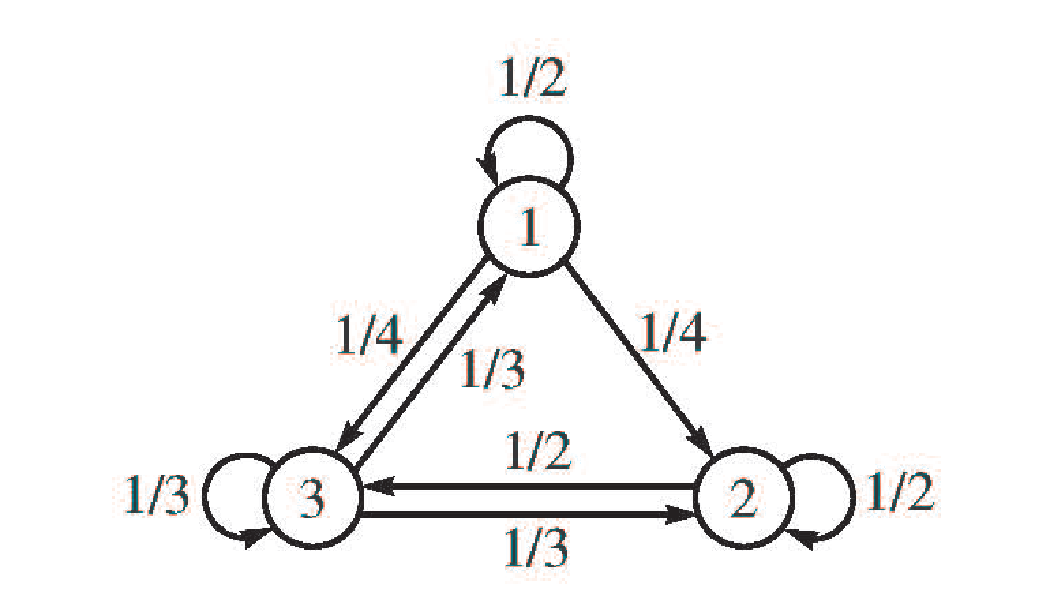
\includegraphics[height=1.5in]{4_newp4_1}}
\caption{Diagram of the random walk in Problem~\ref{newp4_1}.
\label{fig_newp4_1}}
\end{figure}

\section{The Transpose}

If $A$ is an $m\times n$ matrix, then its transpose $A^T$ is the matrix obtained
by flipping $A$ about its diagonal. So the columns of $A^T$ are the rows
of $A$ (in the same order) and vice versa. For example, if
\[
A = \left[\matrix{1&2&3\cr 4&5&6\cr}\right]
\]
then
\[
A^T = \left[\matrix{1&4\cr 2&5\cr 3&6\cr}\right]
\]
Another way of saying this is that the $i,j$th entry of $A^T$ 
is the same as the ${j,i}$th entry of $A$, that is,
\[
a_{i,j}^T = a_{j,i}.
\]

There are two important formulae to remember for the transpose of a matrix.
The first gives a relation between the transpose and the dot product.
If $A$ is an $m\times n$ matrix, then for every $\xx\in\RR^n$ and $\yy\in\RR^m$ 
we have
\begin{equation}
\label{eq_transposedefn}
\yy\cdot (A\xx) = (A^T\yy)\cdot\xx
\end{equation}
The proof of this formula is a simple calculation.
\begin{eqnarray*}
\yy\cdot (A\xx)&=&\sum_{i=1}^{m}y_i \left(\sum_{j=1}^{n}a_{i,j} x_j\right) \\
&=&\sum_{i=1}^{m}\sum_{j=1}^{n}y_i a_{i,j} x_j \\
&=&\sum_{j=1}^{n}\sum_{i=1}^{m}a^T_{j,i} y_i  x_j \\
&=&\sum_{j=1}^{n}\left(\sum_{i=1}^{m}a^T_{j,i} y_i\right)  x_j \\
&=&(A^T\yy)\cdot\xx
\end{eqnarray*}
In fact, the formula (\ref{eq_transposedefn}) could be used to define 
the transpose.
Given $A$, there is exactly one matrix $A^T$ for which 
(\ref{eq_transposedefn})
is true for every $\xx$ and $\yy$, and this matrix is the transpose.

The second important formula relates the transpose of a product of matrices
to the transposes of each one. For two matrices $A$ and $B$ such that $AB$ is defined 
the formula reads
\begin{equation}
\label{eq_transposeprod}
(AB)^T = B^TA^T
\end{equation}
Notice that the order of the factors is reversed on the right side.
To see why (\ref{eq_transposeprod}) is true, notice that on the one hand
\[
\yy\cdot (AB\xx) = ((AB)^T\yy)\cdot\xx
\]
while on the other hand
\[
\yy\cdot (AB\xx) = \yy\cdot (A(B\xx)) = (A^T\yy)\cdot(B\xx) = (B^TA^T\yy)\cdot \xx
\]
Thus $((AB)^T\yy)\cdot\xx=(B^TA^T\yy)\cdot \xx$ for every $\xx$ and $\yy$.
This can only be true if (\ref{eq_transposeprod}) holds. 

\subsection{MATLAB}

The MATLAB operator {\tt '} can be used to take the transpose of a 
matrix. 

\subsection{Problems}

\begin{problem}
\label{op3_15}
Verify formula (\ref{eq_transposedefn}) for 
$\xx=\left[ \begin{array}{c} x_1 \\ x_2 \\ x_3\end{array} \right]$
$\yy=\left[ \begin{array}{c} y_1 \\ y_2 \end{array} \right]$ and 
\[
A = \left[\matrix{1&2&3\cr 4&5&6\cr}\right]
\]
\end{problem}

\begin{problem}
\label{op3_16}
What is $(A^T)^T$?
\end{problem}

\begin{problem}
\label{op3_17}
Verify (\ref{eq_transposeprod}) for 
\[
A = \left[\matrix{1&2 \cr 3&1\cr} \right] \mbox{\ and \ }
B = \left[\matrix{1&2&3\cr 4&5&6\cr}\right]
\]
\end{problem}

\begin{problem}
\label{op3_18}
Show that if $A$ and $B$ are both $m\times n$ matrices
such that $\yy\cdot (A\xx) = \yy\cdot(B\xx)$ for every $\yy\in\RR^m$ and
every $\xx\in\RR^n$, then $A=B$.
\end{problem}

\begin{problem}
\label{op3_19}
Show that if you think of (column) vectors in $\RR^n$ as $n\times 1$ matrices
then
\[
\xx \cdot \yy = \xx^T \yy
\]
Now use this formula and (\ref{eq_transposeprod}) to derive 
(\ref{eq_transposedefn}). 
\end{problem}

\section{Matrix Inverses}

To solve the (scalar) equation
\[
ax=b
\]
for $x$ we simply multiply both sides by $a^{-1}={{1}\over{a}}$. Then,
since $a^{-1}a=1$, we find
\[
x=a^{-1}b.
\]
Of course, if $a=0$ this doesn't work, since we cannot divide by zero. In
fact, if $a=0$ the equation $ax=b$ either has no solutions, if $b\ne 0$, or
infinitely many solutions (every value of $x$), if $b = 0$.

We have seen that a system of linear equations can be rewritten
\[
A\xx = \bb
\]
where is $A$ is a known matrix $\xx$ is the unknown vector to be
solved for, and $\bb$ is a known vector. Suppose we could find an
inverse matrix $B$ (analogous to $a^{-1}$) with the property that
$BA=I$ (recall that $I$ denotes the identity matrix). Then we could
matrix multiply both sides of the equation by $B$ yielding
\[
BA\xx = B\bb
\]
But $BA\xx = I\xx = \xx$, so $\xx=B\bb$. Thus there is a unique
solution and we have a formula for it.

Just as in the numerical case, where $a$ could be zero, we can't
expect to find an inverse matrix in all cases. After all, we know that
there are linear systems of equations with no solutions and with
infinitely many solutions. In these situations there can be no inverse
matrix.

When considering matrix inverses, we will always assume that we are
dealing with square (i.e., $n\times n$) matrices.

\begin{definition}
If $A$ is an $n\times n$ matrix, then $B$ is
called the {\em inverse} of $A$, and denoted $B=A^{-1}$, if 
\[
BA=I
\] 
where $I$ is the $n\times n$ identity matrix (with each diagonal entry
equal to $1$ and all other entries $0$).
\end{definition}

Here is an example. Suppose 
\[
A=\left[\matrix{2&1\cr 5&3\cr}\right]
\] 
then the inverse matrix is
\[
B=A^{-1}=\left[\matrix{3&-1\cr -5&2\cr}\right]
\]
since
\[
\left[\matrix{2&1\cr 5&3\cr}\right]\left[\matrix{3&-1\cr -5&2\cr}\right]
=\left[\matrix{6-5&3-3\cr 10-10&-5+6\cr}\right]=
\left[\matrix{1&0\cr 0&1\cr}\right]
\]
This means that to solve the linear equation
\[
\matrix{
2x_1 &+ x_2 &= 2\cr
5x_1 &+ 3x_2 &= 4\cr
}
\]
we write it as a matrix equation
\[
\left[\matrix{2&1\cr 5&3\cr}\right]
\left[\matrix{x_1\cr x_2\cr}\right]
\left[\matrix{2\cr 4\cr}\right]
\]
and then multiply both sides by the inverse to obtain
\[
\left[\matrix{x_1\cr x_2\cr}\right]
=\left[\matrix{3&-1\cr -5&2\cr}\right]
\left[\matrix{2\cr 4\cr}\right]=
\left[\matrix{2\cr -2\cr}\right]
\]

Here is an example of a matrix that doesn't have an inverse. Let
\[
A=\left[\matrix{1&0\cr 0&0\cr}\right].
\]
To see that $A$ doesn't have an inverse, notice that the homogeneous
equations $A\xx=\zv$ has a non-zero solution $\xx=\left[\matrix{0\cr
1\cr}\right]$. If $A$ had an inverse $B$, then we could multiply both
sides of the equation $A\xx=\zv$ by $B$ to obtain $\xx=B\zv=\zv$. But
this is false. Therefore there cannot be an inverse for $A$.

Clearly, having an inverse is somehow connected to whether or not
there are any non-zero solutions of the homogeneous equation
$A\xx=\zv$. Recall that $A\xx=\zv$ has only the zero solution
precisely when $A\xx=\bb$ has a unique solution for any $\bb$.

Let $A$ be an $n\times n$ matrix. The following conditions are
equivalent:

\begin{enumerate}[(1)]
\item $A$ is invertible. \par
\item The equation $A\xx=\bb$ always has a unique solution.\par
\item The equation $A\xx=\zv$ has as the only solution $\xx=\zv$.\par
\item The rank of $A$ is $n$.\par
\item The reduced form of $A$ is as shown in Figure~\ref{fig_hermite3}.
\end{enumerate}

\begin{figure}
\centerline{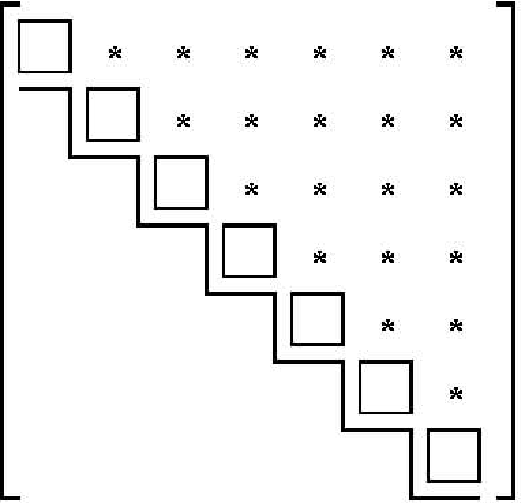
\includegraphics[height=1.5in]{4_hermite3}}
\caption{Diagram of the reduced form of an invertible matrix.
\label{fig_hermite3}}
\end{figure}

We already know that the conditions (2), (3), (4) and (5) are all
equivalent.  We also just have seen that if $A$ is invertible with
inverse $B$, then the solution of $A\xx=\bb$ is $\xx=B\bb$ so it
exists and since we have a formula for it, it is unique.

So we just have to show that if $A\xx=\bb$ always has a unique solution, 
then $A$ has an inverse. Consider the transformation that takes a vector
$\bb$ to the unique solution $\xx$ of $A\xx=\bb$, {em i.e.}, $T\bb = \xx$. 
It is easy to check that this
is a linear transformation, since if $T\bb_1 = \xx_1$, i.e., $A\xx_1=\bb_1$ 
and $T\bb_2 = \xx_2$, i.e., $A\xx_2=\bb_2$, then $A(t_1\xx_1+t_2\xx_2)=
t_1A\xx_1+t_2A\xx_2=t_1\bb_1+t_2\bb_2$, so that $T(t_1\bb_1+t_2\bb_2)=
t_1\xx_1+t_2\xx_2 = t_1T\bb_1+t_2T\bb_1$
Since $T$ is a linear transformation, it is given by some matrix $B$, and
since $T(A\xx)=\xx$, we must have $BA\xx=\xx$ which implies that $BA$ is
the identity matrix.

Going back to our first example, 
notice that not only is $BA=I$, but $AB=I$ too,
since 
\[
\left[\matrix{3&-1\cr -5&2\cr}\right]\left[\matrix{2&1\cr 5&3\cr}\right]
=\left[\matrix{6-5&-2+2\cr 15-15&-5+6\cr}\right]=
\left[\matrix{1&0\cr 0&1\cr}\right]
\]
For a general choice of $A$ and $B$, $BA$ need not be equal to $AB$.
But if $B$ is the inverse of $A$, then it {\em is} always true that
$AB=BA=I$.

To see this, suppose that $A$ is invertible with $BA=I$ but we don't know
yet whether $AB=I$. So what we need to show is that for every vector $\xx$,
$AB\xx=\xx$. First notice that if $A$ is invertible, then any vector $\xx$
can be written in the form $A\yy$ for some $\yy$, since this is just the same
as saying that the equation $A\yy=\xx$ has a solution $\yy$. Thus 
$AB\xx=ABA\yy=AI\yy=A\yy=\xx$.

\subsection{Computing the inverse}

How can we compute the inverse of an $n\times n$ matrix $A$? Suppose
that $A$ is invertible and $B$ is the inverse. Then $AB=I$. We can
rewrite this equation as follows.  Think of the columns of $B$ as
being column vectors so that
\[
B=\Bigg[\bb_1\Bigg|\bb_2\Bigg|\cdots\Bigg|\bb_n\Bigg]
\]
Then the rules of matrix multiplication imply that 
\[
AB = \Bigg[A\bb_1\Bigg|A\bb_2\Bigg|\cdots\Bigg|A\bb_n\Bigg]
\]
Now the identity matrix can also be written as a matrix of column
vectors. In this case the $k$th column is simply the matrix with zeros
everywhere except for a $1$ in the $k$th place, in other words the
vector $\eee_k$. Thus
\[
I=\Bigg[\eee_1\Bigg|\eee_2\Bigg|\cdots\Bigg|\eee_n\Bigg]
\]

So if $AB=I$ then the $n$ equations
\begin{eqnarray*}
A\bb_1&=&\eee_1 \\
A\bb_2&=&\eee_2 \\
&\vdots& \\
A\bb_n&=&\eee_n
\end{eqnarray*}
hold. If we solve each of these equations for $\bb_1$, $\bb_2$,
$\ldots$, $\bb_n$, then we have found the inverse $B$.

Here is a simple example. Suppose we want to find the inverse for 
\[
A=\left[\matrix{2&1\cr 5&3\cr}\right].
\]
According to our discussion, we must solve $A\bb_1=\eee_1$ and
$A\bb_2=\eee_2$.  The augmented matrix for $A\bb_1=\eee_1$ is
\[
\left[\matrix{2&1\cr 5&3\cr}\right.\left|\matrix{1\cr0}\right]
\]
We now perform a sequence of row operations. First divide the first
row by $2$.  This gives
\[
\left[\matrix{1&1/2\cr 5&3\cr}\right.\left|\matrix{1/2\cr0}\right].
\]
Now subtract $5$ times the first row from the second row. This gives
\[
\left[\matrix{1&1/2\cr 0&1/2\cr}\right.\left|\matrix{1/2\cr -5/2}\right].
\]
Now subtract the second row from the first row. This gives
\[
\left[\matrix{1&0\cr 0&1/2\cr}\right.\left|\matrix{3\cr -5/2}\right].
\]
Finally, multiply the second row by $2$. This gives
\[
\left[\matrix{1&0\cr 0&1\cr}\right.\left|\matrix{3\cr -5}\right].
\]
Therefore $\bb_1= \left[\matrix{3\cr -5}\right]$
The augmented matrix for $A\bb_2=\eee_2$ is 
\[
\left[\matrix{2&1\cr 5&3\cr}\right.\left|\matrix{0\cr 1}\right]
\]
We now perform a sequence of row operations. First divide the first row by $2$.
This gives
\[
\left[\matrix{1&1/2\cr 5&3\cr}\right.\left|\matrix{0\cr1}\right].
\]
Now subtract $5$ times the first row from the second row. This gives
\[
\left[\matrix{1&1/2\cr 0&1/2\cr}\right.\left|\matrix{0\cr 1}\right].
\]
Now subtract the second row from the first row. This gives
\[
\left[\matrix{1&0\cr 0&1/2\cr}\right.\left|\matrix{-1\cr 1}\right].
\]
Finally, multiply the second row by $2$. This gives
\[
\left[\matrix{1&0\cr 0&1\cr}\right.\left|\matrix{-1\cr 2}\right].
\]
Therefore $\bb_2= \left[\matrix{-1\cr 2}\right]$. So 
\[
B=\Big[\bb_1\Big|\bb_2\Big] = \left[\matrix{3&-1\cr-5&2\cr}\right]
\]
Notice that we performed {\em exactly the same sequence of row
operations} in finding $\bb_1$ and $\bb_2$. This is because the row
operations only depend on the left side of the augmented matrix, in
other words, the matrix $A$.  If we used this procedure to find the
inverse of an $n\times n$ matrix, we would end up doing exactly the
same row operations $n$ times. Clearly this is a big waste of effort!
We can save a lot of work by solving all the equations at the same
time. To do this we make a super-augmented matrix with both right
sides.
\[
\left[\matrix{2&1\cr 5&3\cr}\right.\left|\matrix{1&0\cr0&1}\right]
\]
Now we only have to go through the sequence of row operations once, keeping
track of both right sides simultaneously. Going through the same sequence,
we obtain
\[
\left[\matrix{1&1/2\cr 5&3\cr}\right.\left|\matrix{1/2&0\cr0&1}\right].
\]
\[
\left[\matrix{1&1/2\cr 0&1/2\cr}\right.\left|\matrix{1/2&0\cr -5/2&1}\right].
\]
\[
\left[\matrix{1&0\cr 0&1/2\cr}\right.\left|\matrix{3&-1\cr -5/2&1}\right].
\]
\[
\left[\matrix{1&0\cr 0&1\cr}\right.\left|\matrix{3&-1\cr -5&2}\right].
\]
Notice that the vectors $\bb_1$ and $\bb_2$ are automatically arranged
as columns on the right side, so the matrix on the right is the
inverse $B$.

The same procedure works for any size of square matrix. To find the
inverse of $A$ form the super-augmented matrix $[A|I]$. Then do a
sequence of row operations to reduce $A$ to the identity. If the
resulting matrix is $[I|B]$ then $B$ is the inverse matrix.

What happens if $A$ doesn't have an inverse? In this case it will be
impossible to reduce $A$ to the identity matrix, since the rank of $A$
is less than $n$.  So the procedure will fail, as it must.

As another example, let us now compute the inverse of an arbitrary
invertible $2\times 2$ matrix
\[
A=\left[\matrix{a&b\cr c&d\cr}\right].
\]
We will see that $A$ is invertible precisely when its determinant
$\Delta=ad-bc$ is non-zero. So let's assume this is the case, and do the
computation.  To start with, let's assume that $ac\ne 0$. Then neither
$a$ or $c$ are zero.  Here is the sequence of row transformations.
\[
\left[\matrix{a&b\cr c&d\cr}\right.\left|\matrix{1&0\cr 0&1}\right]
\]
\[
\left[\matrix{ac&bc\cr ac&ad\cr}\right.\left|\matrix{c&0\cr 0&a}\right]
\matrix{c(1)\cr a(2)}
\]
Notice that multiplication by $a$ and by $c$ would not be legal row
transformations if either $a$ or $c$ were zero.
\[
\left[\matrix{ac&bc\cr 0&ad-bc\cr}\right.\left|\matrix{c&0\cr -c&a}\right]
\matrix{ \cr (2)-(1)}
\]
\[
\left[\matrix{1&b/a\cr 0&1\cr}\right.\left|\matrix{1/a&0\cr -c/\Delta
   &a/\Delta}\right]
\matrix{(1/ac)(1) \cr (1/\Delta)(2)}
\]
\[
\left[\matrix{1&0\cr 0&1\cr}\right.\left|\matrix{d/\Delta
   &-b/\Delta\cr -c/\Delta&a/\Delta}\right]
\matrix{(1)-(b/a)(2) \cr (1/\Delta)(2)}
\]
Thus the inverse matrix is 
\[
A^{-1}= {{1}\over{ad-bc}}\left[\matrix{d&-b\cr -c&a}\right].
\]
This was derived under the additional assumption that $ac\ne
0$. However one can check directly that the same formula works, so
long as $\Delta=ad-bc\ne0$.

\subsection{Inverses of Products}

If both $A$ and $B$ are invertible, then so is $AB$. The inverse of
$AB$ is given by $B^{-1}A^{-1}$. To check this, simply compute
\[
ABB^{-1}A^{-1}=AIA^{-1}=AA^{-1}=I.
\]

If one of $A$ or $B$ is not invertible then $AB$ is not invertible. To
see this recall that a matrix $C$ is not invertible exactly whenever
there is a non-zero solution $\xx$ to $C\xx=\zv$.  If $B$ is not
invertible, then there is a non-zero vector $\xx$ with $B\xx=\zv$.
Then $AB\xx=A\zv=\zv$ so $AB$ is not invertible too.  If $B$ is
invertible, but $A$ is not, then there is a non-zero $\xx$ with
$A\xx=0$.  Let $\yy=B^{-1}\xx$. Since $B^{-1}$ is invertible, $\yy$
cannot be zero. We have $AB\yy=ABB^{-1}\xx=A\xx=\zv$ so $AB$ is not
invertible.

\subsection{MATLAB}

If {\tt A} is an invertible $n \times n$ matrix then the MATLAB 
command {\tt inv(A)} will return its inverse. A system of linear 
equations corresponding to $A \xx = \bb$ where {\tt A} is an invertible 
$n \times n$ matrix and $\bb$ is a column vector with $n$ 
components can be solved with the command 
\begin{verbatim}
x = A\b
\end{verbatim}
Note that if {\tt A} is not square or {\tt A} is square but not invertible 
the corresponding system cannot be solved in this way. In this case, 
use the MATLAB command {\tt rref} on the augmented matrix of the 
system as described in Chapter 3. 

\subsection{Problems}

\begin{problem}
\label{op3_22}
Which of the following matrices are invertible?
\begin{enumerate}[(a)]
\item $\left[\matrix{1&2\cr3&4\cr}\right]$
\item $\left[\matrix{1&2&3\cr0&3&4\cr0&1&1\cr}\right]$
\item $\left[\matrix{1&2&3\cr0&3&4\cr0&1&2\cr}\right]$
\end{enumerate}
\end{problem}

\begin{problem}
\label{op3_23}
Find the inverse for
\[
\left[\matrix{1&2\cr3&5\cr}\right]
\]
\end{problem}

\begin{problem}
\label{op3_24}
Determine which of these matrices are invertible, and find the inverse
for the invertible ones.
\begin{enumerate}[(a)]
\item $\left[\matrix{2&3&-1\cr1&2&3\cr-1&-1&4\cr}\right]$
\item $\left[\matrix{1&-1&1\cr-1&2&-1\cr2&-1&1\cr}\right]$
\item $\left[\matrix{1&1&1\cr1&2&3\cr1&4&9\cr}\right]$
\item $\left[\matrix{2&1&4\cr3&2&5\cr0&-1&1\cr}\right]$
\item $\left[\matrix{1&0&a\cr0&1&0\cr0&0&1\cr}\right]$
\item $\left[\matrix{1&a&b\cr0&1&c\cr0&0&1\cr}\right]$
\end{enumerate}
\end{problem}

\begin{problem}
\label{2009_a8_1}
The following matrices are invertible. Find their inverses.\\
$$
A=\left[\begin{array}{ccc}1&1&1\\ 0&2&3\\ 5&5&1\end{array}\right], \quad
B=\left[\begin{array}{cccc}1&2&-3&1\\ -1&3&-3&-2\\ 2&0&1&5\\ 3&1&-2&5 \end{array}\right].
$$
\end{problem}

\begin{problem}
\label{2009_a8_2}
Consider the system
$$ \left\{
\begin{array}{cc}
&x+5z=6\\
&x-2y+3z=14\\
&2x+y-3z=-2
\end{array}
\right.
$$
\begin{enumerate}
\item Write the above system in the matrix-form, in other words  find a matrix $A$ such that  $A\mathbf{x}=\left[\begin{array}{c}6\\14\\ -2 \end{array}\right]$.
\item Find the inverse of $A$, if possible.
\item How many solutions the system have? Write them all down.
\end{enumerate}
\end{problem}

\section{Determinants}

\subsection{Definition of Determinants}

We have already encountered determinants for $2\times 2$ and $3\times
3$ matrices. For $2\times 2$ matrices
\[
\det\left[\matrix{a_{1,1}&a_{1,2}\cr a_{2,1}&a_{2,2}\cr}\right]
=a_{1,1}a_{2,2}-a_{1,2}a_{2,1}.
\]
For $3\times 3$ matrices we can define the determinant by expanding along the
top row:
\[
\det\left[\matrix{
	a_{1,1}&a_{1,2}&a_{1,3}\cr
	a_{2,1}&a_{2,2}&a_{2,3}\cr
	a_{3,1}&a_{3,2}&a_{3,3}\cr
}\right]
 = a_{1,1}\det\left[\matrix{a_{2,2}&a_{2,3}\cr a_{3,2}&a_{3,3}\cr}\right]
- a_{1,2}\det\left[\matrix{a_{2,1}&a_{2,3}\cr a_{3,1}&a_{3,3}\cr}\right]
+ a_{1,3}\det\left[\matrix{a_{2,1}&a_{2,2}\cr a_{3,1}&a_{3,2}\cr}\right]
\]
If we multiply out the $2\times 2$ determinants in this definition we
arrive at the expression
\[
\det\left[\matrix{
	a_{1,1}&a_{1,2}&a_{1,3}\cr
	a_{2,1}&a_{2,2}&a_{2,3}\cr
	a_{3,1}&a_{3,2}&a_{3,3}\cr
}\right]=
a_{1,1}a_{2,2}a_{3,3}-a_{1,1}a_{2,3}a_{3,2} 
+ a_{1,2}a_{2,3}a_{3,1}-a_{1,2}a_{2,1}a_{3,3} 
+ a_{1,3}a_{2,1}a_{3,2}-a_{1,3}a_{2,2}a_{3,1}
\]
We now make a similar definition for an $n\times n$ matrix. Let $A$ be an 
$n\times n$ matrix. Define $M_{i,j}$ to be the $(n-1)\times (n-1)$ matrix
obtained by crossing out the $i$th row and the $j$th column. So, for example,
if
\[
A=\left[\matrix{1&2&3&4\cr 5&6&7&8\cr 9&0&1&2\cr 3&4&5&6\cr}\right]
\]
then
\[
M_{1,2}=\left[\matrix{ \times &\times &\times &\times\cr 5&\times&7&8\cr 9&\times&1&2\cr 3&\times&5&6\cr}\right]
=\left[\matrix{5&7&8\cr 9&1&2\cr 3&5&6\cr}\right]
\]

We now define the determinant of an $n\times n$ matrix $A$ to be
\[
\det(A) = a_{1,1}\det(M_{1,1})-a_{1,2}\det(M_{1,2})+ \cdots \pm
a_{1,n}\det(M_{1,n}) = \sum_{j=1}^n (-1)^{j+1}a_{1,j}\det(M_{1,j}).
\]
Of course, this formula still contains determinants on the right hand
side.  However, they are determinants of $(n-1)\times(n-1)$
matrices. If we apply this definition to those determinants we get a
more complicated formula involving $(n-2)\times (n-2)$ matrices, and
so on, until we arrive at an extremely long expression (with $n!$
terms) involving only numbers.

Calculating an expression with $n!$ is completely impossible, even with the
fastest computers, when $n$ gets reasonable large. For example
$100! \approx 10^{158}$.
Yet, your computer at home can compute the determinant of a $100\times
100$ matrix in less than a second. The secret, of course, is to compute the
determinant in a different way. We start by computing the determinant of 
triangular matrices.

\subsection{Determinants of Triangular matrices}

Recall that triangular matrices are matrices whose entries above or
below the diagonal are all zero. For $2\times 2$ matrices
\[
\det\left[\matrix{a_{1,1}&a_{1,2}\cr 0&a_{2,2}\cr}\right]
=a_{1,1}a_{2,2}-a_{1,2}0=a_{1,1}a_{2,2}
\]
and
\[
\det\left[\matrix{a_{1,1}&0\cr a_{2,1}&a_{2,2}\cr}\right]
=a_{1,1}a_{2,2}-0a_{2,1}=a_{1,1}a_{2,2}
\]
so the determinant is the product of the diagonal elements. For $3\times 3$
matrices
\begin{eqnarray*}
\det\left[\matrix{
	a_{1,1}&0&0\cr
	a_{2,1}&a_{2,2}&0\cr
	a_{3,1}&a_{3,2}&a_{3,3}\cr
}\right]
&=& a_{1,1}\det\left[\matrix{a_{2,2}&0\cr a_{3,2}&a_{3,3}\cr}\right]
- 0+0 \\
&=& a_{1,1}a_{2,2}a_{3,3}
\end{eqnarray*}
A similar expansion shows that the determinant of an $n\times n$ lower
triangular matrix is the product of the diagonal elements. For upper
triangular matrices we have
\[
\det\left[\matrix{
	a_{1,1}&a_{1,2}&a_{1,3}\cr
	0&a_{2,2}&a_{2,3}\cr
	0&0&a_{3,3}\cr
}\right]
= a_{1,1}\det\left[\matrix{a_{2,2}&a_{2,3}\cr 0&a_{3,3}\cr}\right]
- a_{1,2}\det\left[\matrix{0&a_{2,3}\cr 0&a_{3,3}\cr}\right]
+ a_{1,3}\det\left[\matrix{0&a_{2,2}\cr 0&0\cr}\right]
\]
Since we already know that the determinant of a $2\times 2$ triangular
matrix is the product of the diagonals, we can see easily that the last two
terms in this expression are zero. Thus we get
\begin{eqnarray*}
\det\left[\matrix{
	a_{1,1}&a_{1,2}&a_{1,3}\cr
	0&a_{2,2}&a_{2,3}\cr
	0&0&a_{3,3}\cr
}\right]
&=& a_{1,1}\det\left[\matrix{a_{2,2}&a_{2,3}\cr 0&a_{3,3}\cr}\right] \\
&=& a_{1,1}a_{2,2}a_{3,3}
\end{eqnarray*}
Once we know that the determinant of a $3\times 3$ upper triangular
matrix is the product of the diagonal elements, we can do a similar
calculation to the one above to conclude that determinant of a
$4\times 4$ upper triangular matrix is the product of the diagonal
elements, and so on.

Thus, the determinant of any (upper or lower) triangular $n\times n$
matrix is the product of the diagonal elements.

We know that an arbitrary $n\times n$ matrix can be reduced to an
upper (or lower) triangular matrix by a sequence of row
operations. This is the key to computing the determinant
efficiently. We need to determine how the determinant of a matrix
changes when we do an elementary row operation on it.

\subsection{Summary of determinant calculation rules}

We summarize the results on determinant calculation shown in more detail 
in the additional topics sections~\ref{sec:dettheory1} to~\ref{sec:dettheory7} below. 
The first three rules below show how a determinant changes when row 
operations are applied to it. This can be used to simplify determinant calculation as 
shown in the next section. In the statements below, $A$ is a square matrix. 
\begin{enumerate}
\item If $B$ is obtained from $A$ by multiplying {\em one} row of $A$ by the 
constant $c$ then $\det(B) = c \det(A)$.
\item If $B$ is obtained from $A$ by switching two rows of $A$ then 
$\det(B) = - \det(A)$.
\item If $B$ is obtained from $A$ by adding a multiple of one row to another then 
$\det(B) = \det(A)$
\item $\det(A)=0$ if and only if $A$ is not invertible.
\item For all square matrices $B$ of the same size as $A$, 
$\det(AB) = \det(A) \det(B)$.
\item $\det(A^T) = \det(A)$. 
\end{enumerate}

\subsection{Calculation of determinant using row operations}

We can now use elementary row operations to compute the determinant of
\[
\left[\matrix{1&2&3\cr 1&2&1\cr 2&3&0}\right]
\]
The sequence of row operations that transforms this matrix into an
upper triangular one is (R2)-(R1), (R3)-2(R1), exchange (R2) and
(R3). The determinant doesn't change under the first two
transformations, and changes sign under the third. Thus
\begin{eqnarray*}
\det(\left[\matrix{1&2&3\cr 1&2&1\cr 2&3&0}\right])
&=&\det(\left[\matrix{1&2&3\cr 0&0&-2\cr 2&3&0}\right]) \\
&=&\det(\left[\matrix{1&2&3\cr 0&0&-2\cr 0&-1&-6}\right]) \\
&=&-\det(\left[\matrix{1&2&3\cr 0&-1&-6\cr 0&0&-2\cr}\right]) \\
&=&-(1)(-1)(-2)=-2
\end{eqnarray*}

\subsection{More expansion formulae}

We can use the properties of the determinant to derive alternative
expansion formulae. Recall that we defined the determinant to be
\[
\det(A) = \sum_{j=1}^n (-1)^{j+1}a_{1,j}\det(M_{1,j}).
\]
In other words, we expanded along the top row. Now let's see that we
can expand along other rows as well. Let $A$ be the original matrix
with rows $\aa_1=[a_{1,1},a_{1,2},\ldots,a_{1,n}]$, $\ldots$
$\aa_n=[a_{n,1},a_{n,2},\ldots,a_{n,n}]$.  For example, if $A$ is a
$5\times 5$ matrix then
\[
A=\left[\matrix{\aa_1\cr \aa_2\cr\aa_3\cr\aa_4\cr\aa_5\cr}\right]
\]
Suppose we want to expand along the fourth row. Let $A'$ be the matrix,
where the fourth row of $A$ has been moved to the first row, with all other
rows still in the same order, i.e.,
\[
A'=\left[\matrix{\aa_4\cr \aa_1\cr\aa_2\cr\aa_3\cr\aa_5\cr}\right]
\]
How is the determinant of $A'$ related to the determinant of $A$? We
can change $A$ to $A'$ be a series of row flips as follows:
\[
A=\left[\matrix{\aa_1\cr \aa_2\cr\aa_3\cr\aa_4\cr\aa_5\cr}\right],\quad
\left[\matrix{\aa_1\cr \aa_2\cr\aa_4\cr\aa_3\cr\aa_5\cr}\right],\quad
\left[\matrix{\aa_1\cr \aa_4\cr\aa_2\cr\aa_3\cr\aa_5\cr}\right],\quad
\left[\matrix{\aa_4\cr \aa_1\cr\aa_2\cr\aa_3\cr\aa_5\cr}\right]=A'
\]
We have performed $3$ flips, so $\det(A')=(-1)^3\det(A)=-\det(A)$. 

In general, to move the $i$th row to the top in this way, we must
perform $i-1$ flips, so $\det(A')=(-1)^{i-1}\det(A)$

Notice that $A'$ is a matrix with the properties
\begin{enumerate}[(1)]
\item $a'_{1,j} = a_{i,j}$, since we have moved the $i$th row to the top
\item $M'_{1,j} = M_{i,j}$, since we haven't changed the order of the other
rows.
\end{enumerate}
Therefore
\begin{eqnarray*}
\det(A)&=&(-1)^{i-1}\det(A') \\
&=&(-1)^{i-1}\sum_{j=1}^n (-1)^{j+1}a'_{1,j}\det(M'_{1,j}) \\
&=&(-1)^{i-1}\sum_{j=1}^n (-1)^{j+1}a_{i,j}\det(M_{i,j}) \\
&=&\sum_{j=1}^n (-1)^{i+j}a_{i,j}\det(M_{i,j})
\end{eqnarray*}
This is the formula for expansion along the $i$th row.

As an example let's compute the determinant of a $3\times 3$ matrix by
expanding along the second row.
\begin{eqnarray*}
\det\left[\matrix{1&2&3\cr 1&3&1\cr 1&2&1 \cr}\right]
&=&-\det\left[\matrix{2&3\cr 2&1\cr}\right]
+3\det\left[\matrix{1&3\cr 1&1\cr}\right]
-\det\left[\matrix{1&2\cr 1&2\cr}\right] \\
&=&-2+6+3-9-2+2=-2
\end{eqnarray*}
The formula for expanding along the $i$th row is handy if the matrix
happens to have a row with many zeros.

Using the fact that $\det(A)=\det(A^T)$ we can also write down
expansion formulae along columns, since the columns of $A$ are the
rows of $A^T$.  We end up with the formula
\[
\det(A)=\sum_{i=1}^n (-1)^{i+j}a_{i,j}\det(M_{i,j})
\]

As an example let's compute the determinant of a $3\times 3$ matrix by
expanding along the second column.
\begin{eqnarray*}
\det\left[\matrix{1&2&3\cr 1&3&1\cr 1&2&1 \cr}\right]
&=&-2\det\left[\matrix{1&1\cr 1&1\cr}\right]
+3\det\left[\matrix{1&3\cr 1&1\cr}\right]
-2\det\left[\matrix{1&3\cr 1&1\cr}\right] \\
&=&-2+2+3-9-2+6=-2
\end{eqnarray*}
The formula for expanding along the $j$th column is handy if the matrix
happens to have a column with many zeros.


\subsection{MATLAB}

The MATLAB command {\tt det(A)} can be used to determine the determinant 
of a square matrix as introduced in Chapter 3. 

\subsection{Problems}

\begin{problem}
\label{op3_27}
Find the determinant of
\[
\left[\matrix{1&1&1&1\cr 1&2&4&8\cr 1&3&9&27\cr 1&4&16&64\cr}\right]
\]
\end{problem}

\begin{problem}
\label{op3_28}
Find the determinant of
\[
\left[\matrix{1&-1&1&-1\cr 1&2&4&8\cr 1&-2&4&-8\cr 1&1&1&1\cr}\right]
\]
\end{problem}

\begin{problem}
\label{2009_a9_1}
Consider the matrix $$A = \left[\begin{array}{cccc} 2&0&2&4\\0&0&3&2\\2&2&4&4\\3&0&6&2\end{array}\right].$$
    \begin{enumerate} \item Find the determinant of $A$ by expanding on the first row.
    \item Find the determinant of $A$ by expanding on the row or column of your choice. This expansion should be simpler than the one used in part (a).
    \end{enumerate}
\end{problem}

\begin{problem}
\label{op3_29}
Compute
\[
\det\left[\matrix{1&0&1\cr 1&2&3\cr 3&0&1\cr}\right]
\]
by expanding along the second row, and by expanding along the third
column. 
\end{problem}

\begin{problem}
\label{2009_a9_2}
Find the determinant of $A$ given above by using row operations to
put $A$ into echelon form. 
\end{problem}

\begin{problem}
\label{2009_a9_3}
We know that the determinant of the $n \times n$ matrix $$\left[\begin{array}{cccc} a_1&&&\\ &a_2&&\\ &&\ddots&\\ &&&a_n \end{array}\right]$$
    is $a_1a_2\cdots a_n$ if the blank entries represent 0.
What is the equivalent formula for the determinant of the $n\times n$ matrix
    $$\left[\begin{array}{cccc} &&&a_n\\&&\rdots&\\&a_2&&\\a_1 \end{array}\right]?$$
Justify your answer. 
\end{problem}

\begin{problem}
\label{2009_a9_4}
Find all values of $\lambda$ for which the matrix $$\left[\begin{array}{ccc} 2-\lambda&1&0\\-1&-\lambda&1\\1&3&1-\lambda\end{array}\right]$$ is not invertible.
\end{problem}

\begin{problem}
\label{2009_a9_5}
Determine whether each of the following statements is true or false. If true, explain briefly why it is true without showing specific examples. If false, explain briefly why it is false or give a simple counterexample, and give a correct statement by making small changes to the underlined text.
    \begin{enumerate}
    \item The determinant of \underline{a square matrix} is the product of the entries on its main diagonal.

    \item For \underline{every matrix $A$}, we have $\det(AA^T) = \det(A^TA)$

    \item If $A$ and $B$ are both invertible $n \times n$ matrices, then \underline{$\det(B^{-1}AB)$} \underline{$= \det(BAB^{-1}) = \det(A)$}.

    \item If an $n\times n$ matrix $A$ is multiplied by a scalar $c$, the determinant of the resulting matrix is \underline{$c\cdot\det(A)$}.

    \item If the column vectors of an $n\times n$ matrix are linearly independent, then the row vectors of the same matrix are also \underline{linearly} \underline{independent}.
    \end{enumerate}
\end{problem}

\section{Additional Topics}

\subsection{Return to Resistor Networks}
\label{sec:retres}

Let us revisit the resistor networks we considered in section~\ref{sec_res_networks}. These
networks consist of resistors and voltage and current sources. The {\em fundamental 
problem} was introduced, which was to write the current through the 
voltage sources and the voltage across current sources in terms of arbitrary 
values of the sources.

\begin{figure}
\centerline{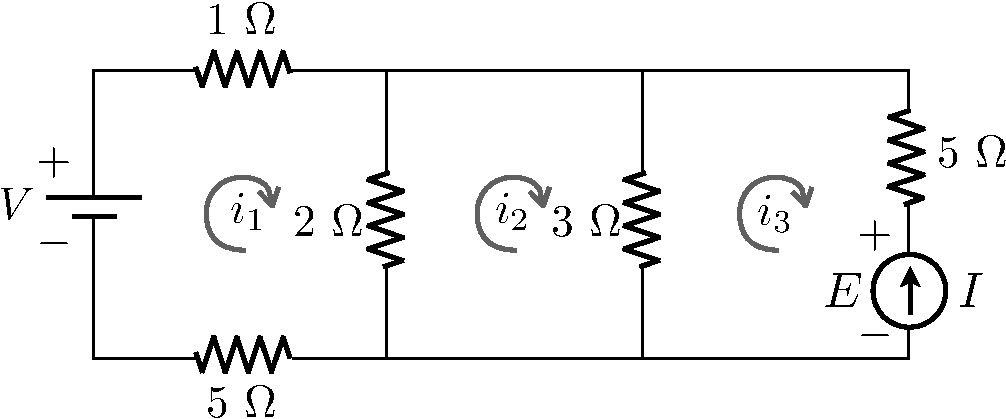
\includegraphics[height=1.5in]{3_resex3}}
\caption{The circuit considered in Example \ref{ex_resex3}. \label{newresf1}}
\end{figure}

Recall example~\ref{ex_resex3} which considered the circuit 
shown again in figure~\ref{newresf1}. The sources are $V$ and $I$. The 
{\em fundamental problem} is to determine $E$ and $J$ (the current through the 
voltage source) in terms of $V$ and $I$. The 
solution found in section~\ref{sec:loop} was 
\begin{eqnarray}
E & = & 6I + V/6 \label{eq:newres1} \\
J & = & -\frac{1}{6} I + \frac{10}{72} V \nonumber  
\end{eqnarray}
This solution can be given in matrix-vector form as 
\begin{equation}
\label{eq:newres2}
\left[ \begin{array}{c} E \\ J \end{array} \right] = 
\left[ \begin{array}{cc} 6 & \frac{1}{6} \\
                                       -\frac{1}{6} & \frac{10}{72} \end{array} \right] 
\left[ \begin{array}{c} I \\ V \end{array} \right]
\end{equation} 
where we will call the $2 \times 2$ matrix in the equation above $F$. It can be shown that 
for any circuit with $n$ sources, the solution of the fundamental problem 
can be written as multiplication by an $n \times n$ matrix. We will show below 
how $F$ can be constructed in a systematic way. Look back to section
\ref{sec:loop} to see how we arrived at (\ref{eq:newres1}). There were three 
parts to the process:
\begin{enumerate}
\item We wrote the linear system for the loop currents and the voltage drop across the 
current source. The equations for the system had the sources $I$ and $V$ in the 
right hand sides.
\item We solved the system symbolically in terms of the right hand side involving $V$ and $I$.
\item We identified the elements of the solution that solved the fundamental problem.  
\end{enumerate} 
We will now describe these three steps by matrix multiplication and do the multiplication 
as an alternate way to determine the matrix $F$ in (\ref{eq:newres2}). Recall that the 
unknowns for the circuit are the three loop currents and $E$, the voltage across the 
current source. Define the intermediate unknown column vector 
\[
{\bf x} = (i_1, i_2, i_3, E)^T.
\] 
Proceeding as in example~\ref{ex_resex3} we find equations for $\bf x$ by considering the 
voltage drops around each elementary loop (the first three equations) around each 
elementary loop (the first three equations) and matching the current through the 
current source (the last equation below):
\begin{equation}
\label{eq:newres3}
\begin{array}{cccccc}
8i_1 & -2i_2 & & & = & V \\
-2i_1 & +5i_2 & -3i_3 & & = & 0 \\
 & -3i_2 & +8i_3 & + E & = & 0 \\
  & & i_3 & & = & -I 
\end{array}
\end{equation}
Here, we did not eliminate $i_3$ from the equations as was done in section~\ref{sec:loop}. 
The system (\ref{eq:newres3}) can be written 
\begin{equation}
\label{eq:newres4}
F_2 {\bf x} = F_1 \left[ \begin{array}{c} I \\ V \end{array} \right]
\end{equation}
where
\[
F_2 = \left[ \begin{array}{cccc} 
8 & -2 & 0 & 0 \\
-2 & 5 & -3 & 0 \\
0 & -3 & 8 & 1 \\
0 & 0 & 1 & 0 
\end{array} \right]
\mbox{\ \ \ and \ \ \ }
F_1 = \left[ \begin{array}{cc}
0 & 1 \\
0 & 0 \\
0 & 0 \\
-1 & 0 
\end{array} \right]
\]
Since $F_2$ is invertible (always true for our approach using loop currents and 
current source voltages as variables) we can proceed from (\ref{eq:newres4}) to 
\begin{equation}
\label{eq:newres5}
{\bf x} = F_2^{-1} F_1 \left[ \begin{array}{c} I \\ V \end{array} \right]
\end{equation}
Now to solve the {\em fundamental problem} of the circuit we want $J=i_1$, the 
current through the voltage sources, and $E$, the voltage across the current 
source. We can write 
\begin{equation}
\label{eq:newres6}
\left[ \begin{array}{c} E \\ J \end{array} \right] = F_3 {\bf x} 
\end{equation}
where 
\[
F_3 = \left[ \begin{array}{cccc} 
0 & 0 & 0 & 1 \\
1 & 0 & 0 & 0 
\end{array} \right].
\]
Combining (\ref{eq:newres5}) and (\ref{eq:newres6}) we obtain 
\begin{equation}
\label{eq:newres7}
\left[ \begin{array}{c} E \\ J \end{array} \right] = F_3 F_2^{-1} F_1 
\left[ \begin{array}{c} I \\ V \end{array} \right]
\end{equation}
Comparing (\ref{eq:newres7}) to (\ref{eq:newres2}) we see that 
\[
F = F_3 F_2^{-1} F_1 
\]
where $F$ is the matrix representing the fundamental solution. Computation 
does indeed show that $F_3 F_2^{-1} F_1$ equals $F$ with 
the matrices defined above. 

The solution of the fundamental problem for any circuit can be written as the product of three 
matrices in the same process described above. We illustrate this with 
a more complex circuit below.

\begin{figure}
\centerline{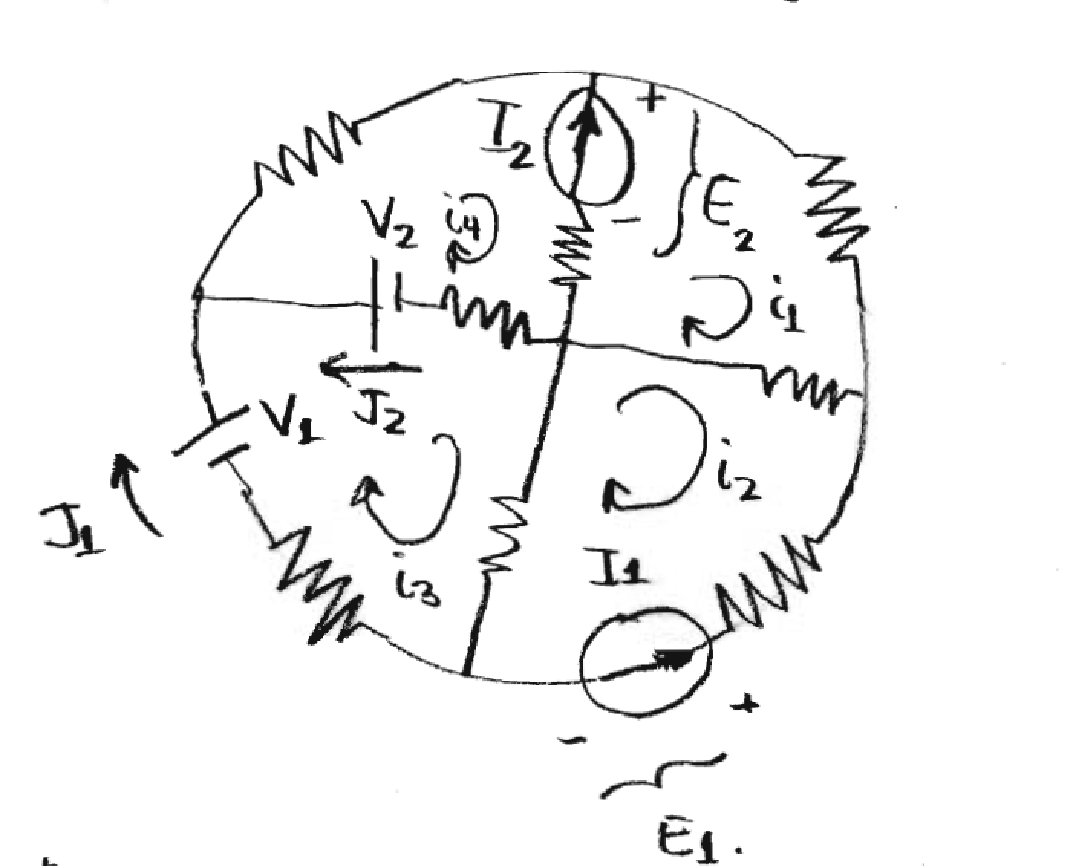
\includegraphics[height=2.5in]{4_newresf1}}
\caption{The circuit considered in Example~\ref{newresex}. All resistors 
are 1$\Omega$. \label{newresf2}}
\end{figure}

\begin{example}
\label{newresex} Find the matrix for the fundamental solution of the 
circuit shown in Figure~\ref{newresf2}.
{\rm 
Here there are four sources $I_1$, $I_2$, $V_1$ and $V_2$ so the 
fundamental problem will be written 
\begin{equation}
\label{eq:newres8}
\left[ \begin{array}{c} E_1 \\ E_2 \\ J_1 \\ J_2  \end{array} \right] =  F 
\left[ \begin{array}{c} I_1 \\ I_2 \\ V_1 \\ V_2  \end{array} \right] 
\end{equation}
where $F$ is a $4 \times 4$ matrix to be determined. The intermediate 
unknowns in the circuit will be 
\[
{\bf x} = (i_1, i_2, i_3, i_4, E_1, E_2)^T
\]
as shown in the figure. Equations for these unknowns are found using the 
loop current method:
\begin{equation}
\label{eq:newres9}
\begin{array}{cccccccc}
3i_1 & -i_2 & & -i_4& & -E_2 &= & 0 \\
-i_1 & +3i_2 & -i_3&  & +E_1& & = & 0 \\
 & -i_2 & +3i_3& -i_4& &  &= & V_1-V_2 \\
-i_1 & & -i_3 & +3i_4& & +E_2& = & V_1 \\
 & i_2 & & & &  & = & -I_1 \\
-i_1 & & & +i_4& & & = & -I_2 \\
\end{array}
\end{equation}
where the first four equations above come from matching voltage 
drops around the four elementary loops and the last two equations come from 
matching the loop currents to the current sources. Note that (\ref{eq:newres9}) 
can be written
\begin{equation}
\label{eq:newres10}
F_2 {\bf x} = F_1 \left[ \begin{array}{c} I_1 \\ I_2 \\ V_1 \\ V_2 \end{array} \right]
\end{equation}
where
\[
F_2 = \left[ \begin{array}{cccccc} 
3 & -1 & 0 & -1 & 0 & -1 \\
-1 & 3 & -1 & 0 & 1 & 0 \\
0 & -1 & 3 & -1 & 0 & 0 \\
-1 & 0 & -1 & 3 & 0 & 1 \\
0 & 1 & 0 & 0 & 0 & 0 \\
-1 & 0 & 0 & 1 & 0 & 0 
\end{array} \right]
\mbox{\ \ \ and \ \ \ }
F_1 = \left[ \begin{array}{cccc}
0 & 0 & 0 & 0 \\
0 & 0 & 0 & 0 \\
0 & 0 & 1 & -1 \\
0 & 0 & 1 & 0 \\
-1 & 0 & 0 & 0 \\
0 & -1 & 0 & 0 \\
\end{array} \right]
\]
Now $J_2 = i_4-i_3$ and $J_1 = i_3$ so we can write
\begin{equation}
\label{eq:newres11}
\left[ \begin{array}{c} E_1 \\ E_2 \\ J_1 \\ J_2  \end{array} \right] =  F_3 {\bf x} 
\end{equation}
where 
\[
F_3 = \left[ \begin{array}{cccccc} 
0 & 0 & 0 & 0 & 1 & 0 \\
0 & 0 & 0 & 0 & 0 & 1 \\
0 & 0 & 1 & 0 & 0 & 0 \\
0 & 0 & -1 & 1 & 0 & 0 
\end{array} \right].
\]
As above we can combine (\ref{eq:newres10}) and (\ref{eq:newres11}) to obtain
\[
\left[ \begin{array}{c} E_1 \\ E_2 \\ J_1 \\ J_2  \end{array} \right] =  F_3 F_2^{-1} F_1 
\left[ \begin{array}{c} I_1 \\ I_2 \\ V_1 \\ V_2  \end{array} \right].
\]
Comparing the equation above to the desired form (\ref{eq:newres8}) we see that the 
fundamental matrix $F$ can be computed as 
\[
F = F_3 F_2^{-1} F_1.
\]
A MATLAB computation with the matrices defined above gives 
\[
F \approx 
\left[ \begin{array}{cccc}
2.1818 & 0.2727 & 0.8182 & -0.4545 \\
0.2727 & 1.9091 & 0.7273 & -0.1818 \\
-0.4545 & -0.1818 & 0.4545 & -0.3636 \\
0.0909 & -0.3636 & -0.0909 & 0.2727 
\end{array} \right]
\]
}
\end{example}

This technique can be used to find the fundamental solution of circuits even if they 
are very large. You can imagine that the process of setting up the 
matrices $F_1$, $F_2$ and $F_3$, computing an approximation of $F_2^{-1}$ and 
multiplying the matrices together can all be automated and done computationally. 

In Chapter 5, fundamental matrices for circuits will be used to investigate the transient 
behaviour of circuits with capacitors and inductors as well as resistors. 


\subsection{Application: General Least Squares}

Let us restate our results from Chapter 3 on minimization of quadratic functions
using matrix notation. A quadratic function of 
\[
\xx = \left[ \begin{array}{c} x_1 \\ \vdots \\ x_n \end{array} \right]
\]
in $\RR^n$ can be written in matrix form as
\[
f(\xx) = \xx \cdot A\xx + \bb\cdot\xx + c
\]
where $A$ is an $n\times n$ matrix and $\bb\in\RR^n$ and $c$ is a number.
The vector containing the partial derivatives can be computed to be
\[
\left[ \begin{array}{c} {\PA f}/{\PA x_1} \\ \vdots \\ 
   {\PA f}/{\PA x_n} \end{array} \right]
= (A + A^T)\xx +\bb
\]
Recall that we made the assumption that $a_{ij}=a_{ji}$ when we considered
this problem before. This property can be stated in compact form as 
$A=A^T$. If this is true then $(A + A^T)=2A$ so
\[
\left[ \begin{array}{c} {\PA f}/{\PA x_1} \\ \vdots \\ 
   {\PA f}/{\PA x_n} \end{array} \right]
= 2A\xx +\bb
\]
To find the minimum value of $f$ (if it exists) we need to find
the value of $\xx$ for which the vector above is zero. In other words,
$\xx$ solves the equation
\[
2A\xx = -\bb.
\]
This is the same equation that we derived before.

\subsection{Least squares solutions}

Let's take another look the situation where a system of linear equations,
which we now can write
\[
B\xx =\cc,
\]
has no solution. Typically this will be the case if there are more
equations than variables, that is, $B$ is an matrix with more rows
than columns. In this case there is no value of $\xx$ that makes
the left side equal the right side. However, we may try to find
the value of $\xx$ for which the right side $B\xx$ is {\it closest} to the left
side $\cc$. 

One way to go about this is to try to minimize distance between
the left and right sides. It is more convenient to minimize
the square of the distance. This quantity can be written
\begin{eqnarray*}
\|B\xx-\cc\|^2 &=& (B\xx-\cc)\cdot(B\xx-\cc) \\
&=&(B\xx)\cdot(B\xx) - (B\xx)\cdot\cc - \cc\cdot(B\xx) + \cc\cdot\cc \\
&=&\xx\cdot(B^TB\xx) - 2(B^T\cc)\cdot\xx + \cc\cdot\cc
\end{eqnarray*}
This is a quadratic function, written in matrix form. 
We want to  use the formula of the previous section 
with $A=B^TB$ and $\bb=B^T\cc$. Before we can do so, we must verify
that $A=B^TB$ satisfies $A^T=A$. This is true because
\[
(A^TA)^T = A^T(A^T)^T = A^T A
\]
Thus the formula of the previous section implies 
that the minimum
occurs at the value of $\xx$ that solves the linear equation
\[
B^TB\xx = B^T\cc
\]
Here we have cancelled a factor of $2$ on each side.

Now let's derive the same result in another way. Think of all the values
of $B\xx$, as $\xx$ ranges through all possible values in $\RR^n$
as forming a (high dimensional) plane in $\RR^m$. Our goal is to find
the value of $\xx$ so that the corresponding value of $B\xx$ on the
plane is closest to $\cc$. Using the analogy to the geometric picture
in three dimensions, we see that the minimum will occur when $B\xx-\cc$
is orthogonal to the plane. This means that the dot product of $B\xx-\cc$
with every vector in the plane, that is, every vector of the form $B\yy$,
should be zero. Thus we have
\[
(B\yy)\cdot(B\xx - \cc) = \zv
\]
for every $\yy\in \RR^n$. This is the same as
\[
\yy\cdot(B^T(B\xx - \cc)) = \yy\cdot(B^TB\xx - B^T\cc) = \zv
\]
for every $\yy\in \RR^n$. This can happen only if
\[
B^TB\xx = B^T\cc
\]
which is the same result we obtained before. 

\subsection{Problems}

\begin{problem}
\label{op3_20}
Find the least squares solution to
\[
\matrix{
x_1 &+ x_2 &= 1\cr
x_1 &&=1\cr
x_1 &+ x_2 &= 0\cr
}
\]
Compare $B\xx$ and $\bb$.
\end{problem}

\begin{problem}
\label{op3_21}
Refer back to the least squares fit example, where we tried to 
find the best
straight line going through a collection of points $(x_i,y_i)$. 
Another way of formulating this problem is this. The line $y=ax+b$
passes through the point $(x_i,y_i)$ if 
\begin{equation}
\label{eq_lsfeqn}
a x_i + b = y_i
\end{equation}
So, saying that the straight line passes through all $n$ points is the
same as saying that $a$ and $b$ solve the system of $n$ linear equations given
by (\ref{eq_lsfeqn})
 for $i = 1, \ldots, n$. Of course, unless the points all actually
lie on the same line, this system of equations has no solutions. Show that
the least squares solution to this problem is the same as we obtained before.
(You may simplify the problem by assuming there are only three points
$(x_1,y_1)$, $(x_2,y_2)$ and $(x_3,y_3)$.)
\end{problem}

\subsection{Elementary matrices}

Recall that there are three row operation that are used in Gaussian
elimination: (1) multiplication of a row by a non-zero number, (2) add
a multiple of one row to another row and (3) exchanging two rows.

It turns out that each elementary row operation can be implemented by
left multiplication by a matrix. In other words, for each elementary
row operation there is a matrix $Q$ such that $QA$ is what you get by
doing that row operation to the matrix $A$.

Here is an example. Suppose 
\[
A=\left[\matrix{1&0&2&1\cr 2&0&0&1\cr 1&2&3&4\cr}\right]
\]
and suppose that the row operation is multiplying the first row by
2. Then the matrix you get by doing that row operation to the matrix
$A$ is
\[
A'=\left[\matrix{2&0&4&2\cr 2&0&0&1\cr 1&2&3&4\cr}\right]
\]
In this case the matrix $Q$ turns out to be 
\[
Q=\left[\matrix{2&0&0\cr 0&1&0\cr 0&0&1\cr}\right]
\]
Since
\[
\left[\matrix{2&0&0\cr 0&1&0\cr 0&0&1\cr}\right]\left[\matrix{1&0&2&1\cr
2&0&0&1\cr 1&2&3&4\cr}\right] = \left[\matrix{2&0&4&2\cr 2&0&0&1\cr
1&2&3&4\cr}\right]
\]
i.e., $QA=A'$.

Now suppose that the elementary row operation is subtracting twice the
first row from the second row. Then the matrix you get by doing that
row operation to the matrix $A$ is
\[
A'=\left[\matrix{1&0&2&1\cr 0&0&-4&-1\cr 1&2&3&4\cr}\right]
\]
In this case the matrix $Q$ turns out to be 
\[
Q=\left[\matrix{1&0&0\cr -2&1&0\cr 0&0&1\cr}\right]
\]
Since
\[
\left[\matrix{1&0&0\cr -2&1&0\cr 0&0&1\cr}\right]
\left[\matrix{1&0&2&1\cr
2&0&0&1\cr 1&2&3&4\cr}\right]=
\left[\matrix{1&0&2&1\cr 0&0&-4&-1\cr 1&2&3&4\cr}\right]
\]
i.e., again, $QA=A'$.

Finally, suppose that the elementary row operation is exchanging the
second and the third rows. Then the matrix you get by doing that row
operation to the matrix $A$ is
\[
A'=\left[\matrix{1&0&2&1\cr 1&2&3&4\cr 2&0&0&1\cr }\right]
\]
In this case the matrix $Q$ turns out to be 
\[
Q=\left[\matrix{1&0&0\cr 0&0&1\cr 0&1&0\cr}\right]
\]
Since
\[
\left[\matrix{1&0&0\cr 0&0&1\cr 0&1&0\cr}\right]
\left[\matrix{1&0&2&1\cr
2&0&0&1\cr 1&2&3&4\cr}\right]=\left[\matrix{1&0&2&1\cr 1&2&3&4\cr 2&0&0&1\cr
}\right]
\]
i.e., again, $QA=A'$.

How can we find the matrices $Q$ (called elementary matrices)? Here is
the procedure. Start with the identity matrix $I$ and do the row
transformation to it. The resulting matrix $Q$ is the matrix that
implements that row transformation by multiplication from the
left. Notice that this is true in the examples above. In the first
example, the row transformation was multiplying the first row by 2. If
you multiply the first row of
\[
I=\left[\matrix{1&0&0\cr 0&1&0\cr 0&0&1\cr}\right]
\]
by two you get 
\[
Q=\left[\matrix{2&0&0\cr 0&1&0\cr 0&0&1\cr}\right].
\]
In the second example, the row transformation was subtracting twice
the first row from the second row. If you subtract twice the second
row from the first row of $I$ by two you get 
\[
Q=\left[\matrix{1&0&0\cr -2&1&0\cr 0&0&1\cr}\right].
\]
In the third example, the row transformation was exchanging the second and
third rows. If you exchange the second and third rows of $I$, you get
\[
\left[\matrix{1&0&0\cr 0&0&1\cr 0&1&0\cr}\right].
\]

Elementary matrices are useful in theoretical studies of the Gaussian
elimination process. We will use them briefly when studying
determinants.

Suppose $A$ is a matrix, and $R$ is its reduced form. Then we can
obtain $R$ from $A$ via a sequence of elementary row operations.
Suppose that the corresponding elementary matrices are $Q_1$, $Q_2$,
$\ldots$, $Q_k$. Then, starting with $A$, the matrix after the first
elementary row operation is $Q_1A$, then after the second elementary
row operation is $Q_2Q_1A$, and so on, until we have
\[
Q_kQ_{k-1}\cdots Q_2Q_1A = R.
\]
Now let us apply the inverse matrices, starting with $Q_k^{-1}$. This gives
\[
Q_k^{-1}Q_kQ_{k-1}\cdots Q_2Q_1A = Q_{k-1}\cdots Q_2Q_1A = Q_k^{-1}R.
\]
Continuing in this way we see that
\[
A = Q_1^{-1}Q_2^{-1}\cdots Q_k^{-1}R
\]

In the special case that $A$ is an $n\times n$ invertible matrix, $A$ can
be reduced to the identity matrix. In other words, we can take $R=I$.
In this case $A$ can be written as a product of elementary matrices.
\[
A = Q_1^{-1}Q_2^{-1}\cdots Q_k^{-1}I=Q_1^{-1}Q_2^{-1}\cdots Q_k^{-1}
\]
Notice that in this case
\[
A^{-1} = Q_kQ_{k-1}\cdots Q_2Q_1.
\]
As an example, let us write the matrix 
\[
A=\left[\matrix{2&1\cr 5&3\cr}\right]
\]
as a product of elementary matrices. The sequence of row transformations
that reduce $A$ to the identity are:
\begin{enumerate}[1)]
\item (1/2)(R1)
\item (R2)-5(R1)
\item (R1)-(R2)
\item 2(R2)
\end{enumerate}

The corresponding elementary matrices and their inverses are
\[
Q_1 = \left[\matrix{1/2&0\cr 0&1\cr}\right]\quad
Q_1^{-1} = \left[\matrix{2&0\cr 0&1\cr}\right]
\]
\[
Q_2 = \left[\matrix{1&0\cr -5&1\cr}\right]\quad
Q_2^{-1} = \left[\matrix{1&0\cr 5&1\cr}\right]
\]
\[
Q_3 = \left[\matrix{1&-1\cr 0&1\cr}\right]\quad
Q_3^{-1} = \left[\matrix{1&1\cr 0&1\cr}\right]
\]
\[
Q_4 = \left[\matrix{1&0\cr 0&2\cr}\right]\quad
Q_4^{-1} = \left[\matrix{1&0\cr 0&1/2\cr}\right]
\]
Therefore 
\[
A=Q_1^{-1}Q_2^{-1}Q_3^{-1}Q_4^{-1}
\] 
or
\[
\left[\matrix{2&1\cr 5&3\cr}\right]=\left[\matrix{2&0\cr 0&1\cr}\right]
\left[\matrix{1&0\cr 5&1\cr}\right]
\left[\matrix{1&1\cr 0&1\cr}\right]
\left[\matrix{1&0\cr 0&1/2\cr}\right]
\]

\subsection{Problems}

\begin{problem}
\label{op3_25}
Each elementary matrix is invertible, and the inverse is also an
elementary matrix. Find the inverses of the three examples of
elementary matrices above.  Notice that the inverse elementary matrix
is the matrix for the row transformation that undoes the original row
transformation.
\end{problem}

\begin{problem}
\label{op3_26}
Write the matrix 
\[
\left[\matrix{2&3&-1\cr1&2&3\cr-1&-1&1\cr}\right]
\]
as a product of elementary matrices.
\end{problem}


\subsection{Exchanging two rows changes the sign of the determinant}
\label{sec:dettheory1}

We start with the elementary row operation of exchanging two rows. For 
$2\times 2$ determinants, 
\[
\det\left[\matrix{a&b\cr c&d\cr}\right] = ad-bc,
\]
while
\[
\det\left[\matrix{c&d\cr a&b\cr}\right] = cb-da = -(ad-bc),
\]
so exchanging two rows changes the sign of the determinant.

We can do a similar calculation for $3\times 3$ matrices. Its a a bit
messier, but still manageable. Again, we find that exchanging two rows
changes the sign of the determinant.

How about the $n\times n$ case? We will assume that we have already
proved the result for the $(n-1)\times (n-1)$ case, and show how we
can use this to show the result for an $n\times n$ matrix. Thus
knowing the result for $2\times 2$ matrices, implies it for $3\times
3$, which in turn implies it for $4\times 4$ matrices, and so on. We
consider three cases, depending on which rows we are
exchanging. Suppose $A$ is the original matrix and $A'$ is the matrix
with two rows exchanged.

\begin{enumerate}[(1)]
\item Exchanging two rows other than the first row: In this case we
cross out the first row and any column from $A'$ we obtain $M'_{1,j}$
which is the same as the matrix $M_{1,j}$ (corresponding to $A$)
except with two of its rows exchanged. Since the size of $M_{1,j}$ is
$n-1$ we know that $\det(M'_{1,j}) = - \det(M_{1,j})$ so
\begin{eqnarray*}
\det(A')&=&\sum_{j=1}^n (-1)^{j+1}a_{1,j}\det(M'_{1,j}) \\
&=&-\sum_{j=1}^n (-1)^{j+1}a_{1,j}\det(M_{1,j}) \\
&=&-\det(A)
\end{eqnarray*}
\item Exchanging the first and second row. Do see that this changes
the sign of the determinant we have to expand the expansion. The
following is a bit sketchy. I'll probably skip it in class, but give
the argument here for completeness. If we expand $M_{1,j}$ we get
\[
\det(M_{1,j}) = \sum_{k=1}^{j-1}(-1)^{k+1}a_{2,k}\det(M_{1,2,j,k})
+ \sum_{k=j+1}^{n}(-1)^{k}a_{2,k}\det(M_{1,2,j,k})
\]
where $M_{1,2,j,k}$ is the matrix obtained from $A$ by deleting the first and 
second rows, and the $j$th and $k$th columns. Inserting this into the expansion
for $A$ gives
\[
\det(A)=\sum_{j=1}^n\sum_{k=1}^{j-1}(-1)^{j+k}a_{1,j}a_{2,k}\det(M_{1,2,j,k})
-\sum_{j=1}^n\sum_{k=j+1}^{n}(-1)^{j+k}a_{1,j}a_{2,k}\det(M_{1,2,j,k})
\]
The sum splits into two parts. Flipping the first two rows of $A$ just
exchanges the two sums. In other words $S-R$ becomes $R-S$ which is
$-(S-R)$. So exchanging the first two rows also changes the sign of
the determinant.
\item Exchanging the first row with the $k$th row. We can effect this
exchange by first exchanging the $k$th and the second row, then
exchanging the first and the second row, then exchanging the $k$th and
the second row again. Each flip changes the determinant by a minus
sign, and since there are three flips, the overall change is by a
minus sign.
\end{enumerate}

Thus we can say that for any $n\times n$ matrix, exchanging two rows changes 
the sign of the determinant. 

One immediate consequence of this fact is that a matrix with two rows
the same has determinant zero. This is because if exchange the two
rows the determinant changes by a minus sign, but the matrix doesn't
change. Thus $\det(A)=-\det(A)$ which is only possible if $\det(A)=0$.

\subsection{The determinant is linear in each row separately}
\label{sec:dettheory2}

To say that the determinant is linear in the $j$th row means that if
we write a matrix as a matrix of row vectors,
\[
A= \left[\matrix{\aa_1\cr\aa_2\cr\vdots\cr\aa_j\cr\vdots\cr\aa_n\cr}\right]
\]
then
\[
\det(\left[\matrix{\aa_1\cr\aa_2\cr\vdots\cr s\bb + t\cc\cr
\vdots\cr\aa_n\cr}\right])
=s\det(\left[\matrix{\aa_1\cr\aa_2\cr\vdots\cr \bb \cr
\vdots\cr\aa_n\cr}\right])
+ t\det(\left[\matrix{\aa_1\cr\aa_2\cr\vdots\cr \cc\cr
\vdots\cr\aa_n\cr}\right])
\]

It is easy to from the expansion formula that the determinant is linear
in the first row. For a $3\times 3$ example we have
\[
\det(
\left[\matrix{sb_1+tc_1&sb_2+tc_2&sb_3+tc_3\cr
a_{2,1}&a_{2,2}&a{2,3}\cr
a_{3,1}&a_{3,2}&a{3,3}\cr}\right]
)
\]
\begin{eqnarray*}
&=& (sb_1+tc_1)\det(M_{1,1}) - (sb_2+tc_2)\det(M_{1,2}) +
(sb_3+tc_3)\det(M_{1.3}) \\
&=&s(b_1\det(M_{1,1}) - b_2\det(M_{1,2}) +
b_3\det(M_{1.3})) \\
& & \quad +
t(c_1\det(M_{1,1}) - c_2\det(M_{1,2}) +
c_3\det(M_{1.3})) \\
&=& s\det(
\left[\matrix{b_1&b_2&b_3\cr
a_{2,1}&a_{2,2}&a{2,3}\cr
a_{3,1}&a_{3,2}&a{3,3}\cr}\right]
)+
t\det(
\left[\matrix{c_1&c_2&c_3\cr
a_{2,1}&a_{2,2}&a{2,3}\cr
a_{3,1}&a_{3,2}&a{3,3}\cr}\right]
) \\
\end{eqnarray*}
A similar calculation can be done for any $n\times n$ matrix to show
linearity in the first row. To show linearity in some other row, we
first swap that row and the first row, then use linearity in the first
row, and then swap back again. So
\begin{eqnarray*}
\det(\left[\matrix{\aa_1\cr\aa_2\cr\vdots\cr s\bb + t\cc\cr
\vdots\cr\aa_n\cr}\right])
&=& -\det(\left[\matrix{s\bb + t\cc\cr\aa_2\cr\vdots\cr \aa_1\cr
\vdots\cr\aa_n\cr}\right]) \\
&=& -s\det(\left[\matrix{\bb\cr\aa_2\cr\vdots\cr \aa_1\cr
\vdots\cr\aa_n\cr}\right]) - t\det(\left[\matrix{\cc\cr\aa_2\cr\vdots\cr \aa_1\cr
\vdots\cr\aa_n\cr}\right]) \\
&=&s\det(\left[\matrix{\aa_1\cr\aa_2\cr\vdots\cr \bb\cr
\vdots\cr\aa_n\cr}\right]) + t\det(\left[\matrix{\aa_1\cr\aa_2\cr\vdots\cr \cc\cr
\vdots\cr\aa_n\cr}\right])
\end{eqnarray*}
Notice that linearity in each row separately does {\bf not} mean that
$\det(A+B)=\det(A)+\det(B)$.

Note that multiplying a row by a constant multiplies the determinant
by the constant. This is a special case of linearity.

\subsection{Adding a multiple of one row to another doesn't change 
the determinant}
\label{sec:dettheory3}

Now we will see that the most often used row operation---adding a
multiple of one row to another---doesn't change the determinant at
all. Let $A$ be an $n\times n$ matrix. Write $A$ as a matrix of rows.
\[
A=\left[\matrix{\aa_1\cr\vdots\cr\aa_i\cr\vdots\cr\aa_j\cr
   \vdots\cr\aa_n\cr}\right]
\]
Adding $s$ times the $i$th row to the $j$th row yields
\[
A'= \left[\matrix{\aa_1\cr\vdots\cr\aa_i\cr\vdots\cr\aa_j+
   s\aa_i\cr\vdots\cr\aa_n\cr}\right]
\]
So
\[
\det(A') =
\det(\left[\matrix{\aa_1\cr\vdots\cr\aa_i\cr\vdots\cr\aa_j+s\aa_i\cr\vdots\cr\aa_n\cr}\right])
=\det(\left[\matrix{\aa_1\cr\vdots\cr\aa_i\cr\vdots\cr\aa_j\cr\vdots\cr\aa_n\cr}\right])
+s
\det(\left[\matrix{\aa_1\cr\vdots\cr\aa_i\cr\vdots\cr\aa_i\cr\vdots\cr\aa_n\cr}\right])
=\det(A)+0
\]
Here we used linearity in a row and the fact that the determinant of a
matrix with two rows the same is zero.

\subsection{The determinant of $QA$}
\label{sec:dettheory4}

To begin, we compute the determinants of the elementary
matrices. Recall that if $A'$ is the matrix obtained from $A$ by an
elementary row operation, then
\begin{enumerate}[(1)]
\item $\det(A') = -\det(A)$ if the row operation is swapping two rows
\item $\det(A') = s\det(A)$ if the row operation is multiplying a row by $s$
\item $\det(A') = \det(A)$ if the row operation is adding a multiple
of one row to another
\end{enumerate}
Recall that the elementary matrices are obtained from the identity
matrix $I$ by an elementary row operation. So we can take $A=I$ and
$A'=Q$ in the formulae above to obtain
\begin{enumerate}[(1)]
\item $\det(Q) = -\det(I)=-1$ if the row operation is swapping two rows
\item $\det(Q) = s\det(I)=s$ if the row operation is multiplying a row by $s$
\item $\det(Q) = \det(I)=1$ if the row operation is adding a multiple
of one row to another
\end{enumerate}
Going back to the first set of formulae, we have that in each case
$A'=QA$. In each case the factor in front of $\det(A)$ is exactly
$\det(Q)$ So we see that in each case
\[
\det(QA)=\det(Q)\det(A).
\]
This formula can be generalized. If $Q_1$, $Q_2$, $\ldots$, $Q_k$ are
elementary matrices then $\det(Q_1Q_2Q_3\cdots
Q_kA)=\det(Q_1)\det(Q_2Q_3\cdots Q_kA) =\det(Q_1)
\det(Q_2)\det(Q_3\cdots Q_kA)$ and so on, so we arrive at the formula
\[
\det(Q_1Q_2Q_3\cdots Q_kA)=\det(Q_1)\det(Q_2)\cdots\det(Q_k)\det(A).
\]

\subsection{The determinant of $A$ is zero exactly when $A$ is 
not invertible}
\label{sec:dettheory5}

Recall that if $R$ denotes the reduced form of $A$, obtained by
performing the sequence of row reductions corresponding to $Q_1$,
$Q_2$, $\ldots$, $Q_k$, then
\[
A= Q_1^{-1}Q_2^{-1}\cdots Q_k^{-1}R
\]
Each $Q_i^{-1}$ is an elementary matrix, therefore
\[
\det(A) = \det(Q_1^{-1})\det(Q_2^{-1})\cdots \det(Q_k^{-1})\det(R)
\]
If $A$ is not invertible, then $R$ has a row of zeros along the
bottom. Thus $R$ is an upper triangular matrix with at least one zero
on the diagonal. The determinant of $R$ is the product of the diagonal
elements so $\det(R)=0$.  Thus $\det(A)=0$ too.

If $A$ is invertible, then we can reduce $A$ to to identity matrix. In
other words, we can take $R=I$. Then $\det(R)=1$. Each
$\det(Q_i^{-1})$ is non-zero too, so $\det(A)\ne 0$.

\subsection{The product formula: $\det(AB)=\det(A)\det(B)$}
\label{sec:dettheory6}

If either $A$ or $B$ is non-invertible, then $AB$ is non-invertible
too. Thus $\det(AB)=0$ and one of $\det(A)$ or $\det(B)$ is zero, so
$\det(A)\det(B)=0$ too. Thus $\det(AB)=\det(A)\det(B)$.

If both $A$ and $B$ are invertible, then
\[
A= Q_1^{-1}Q_2^{-1}\cdots Q_k^{-1}
\]
so
\[
\det(A) = \det(Q_1^{-1})\det(Q_2^{-1})\cdots \det(Q_k^{-1})
\]
and 
\[
B= \tilde Q_1^{-1}\tilde Q_2^{-1}\cdots \tilde Q_j^{-1}
\]
so
\[
\det(B) = \det(\tilde Q_1^{-1})\det(\tilde Q_2^{-1})\cdots \det(\tilde
Q_j^{-1})
\]
Therefore
\[
AB=Q_1^{-1}Q_2^{-1}\cdots Q_k^{-1}\tilde Q_1^{-1}\tilde Q_2^{-1}\cdots
\tilde Q_j^{-1}
\]
so
\[
\det(AB)=\det(Q_1^{-1})\det(Q_2^{-1})\cdots \det(Q_k^{-1}) \det(\tilde
Q_1^{-1})\det(\tilde Q_2^{-1})\cdots \det(\tilde
Q_j^{-1})=\det(A)\det(B)
\]

\subsection{The determinant of the transpose}
\label{sec:dettheory7}

Recall that the transpose $A^T$ of a matrix $A$ is the matrix you get
when you flip $A$ about its diagonal. If $A$ is an $n\times n$ matrix,
so is $A^T$ and we can ask what the relationship between the
determinants of these two matrices is. It turns out that they are the
same.
\[
\det(A^T)=\det(A).
\] 
If $A$ is an upper or lower triangular matrix, this follows from the
fact that the determinant of a triangular matrix is the product of the
diagonal entries. If $A$ is an arbitrary $n\times n$ matrix then the
formula follows from two facts.

\begin{enumerate}[(1)]
\item The transpose of a product of two matrices is given by
$(AB)^T=B^TA^T$. This implies that $(A_1A_2\cdots A_n)^T=A_n^T\cdots
A_2^TA_1^T$.
\item For an elementary matrix $Q$ we have $\det(Q^T)=\det(Q)$.
\end{enumerate}
If you accept these two facts, then we may write
\[
A= Q_1^{-1}Q_2^{-1}\cdots Q_k^{-1}R
\]
where $R$ is upper triangular. Thus
\[
A^T=R^T(Q_k^{-1})^T\cdots (Q_2^{-1})^T(Q_1^{-1})^T
\]
so
\begin{eqnarray*}
\det(A^T)&=&\det(R^T)\det((Q_k^{-1})^T)\cdots \det((Q_1^{-1})^T) \\
&=&\det(R)\det(Q_k^{-1})\cdots \det(Q_1^{-1}) \\
&=&\det(Q_1^{-1})\cdots \det(Q_k^{-1})\det(R) \\
&=&\det(A)
\end{eqnarray*}


\subsection{An impractical formula for the inverse}
\label{sec:cramer1}

We can use the expansion formulae of the previous section to obtain a
formula for the inverse of a matrix $A$. This formula is really only
practical for $3\times 3$ matrices, since for larger matrices, the
work involved in computing the determinants appearing is prohibitive.

We begin with the expansion formula
\[
\det(A)=\sum_{j=1}^n (-1)^{i+j}a_{i,j}\det(M_{i,j})
\]
If $A$ is invertible, then $\det(A)\ne 0$ so we can divide by it to obtain
\[
1=\sum_{j=1}^n a_{i,j}{{(-1)^{i+j}\det(M_{i,j})}\over{\det(A)}}
\]
Now suppose we take the matrix $A$ and replace the $i$th row by the
$k$th row for some $k\ne i$. The resulting matrix $A'$ has two rows
the same, so its determinant is zero. Its expansion is the same as
that for $A$, except that $a_{i,j}$ is replaced by $a_{k,j}$. Thus, if
$k\ne i$
\[
0=\sum_{j=1}^n (-1)^{i+j}a_{k,j}\det(M_{i,j})
\]
Dividing by $\det(A)$ yields
\[
0=\sum_{j=1}^n a_{k,j} {{(-1)^{i+j}\det(M_{i,j})}\over{\det(A)}}
\]

Now let $B$ be the matrix with entries
\[
b_{i,j} = {{(-1)^{i+j}\det(M_{j,i})}\over{\det(A)}}
\]
This turns out to be the inverse $A^{-1}$. 

It gets a bit confusing with all the indices, but let's think about what we
need to show. The $k,i$th entry of the product $AB$ is given by
\begin{eqnarray*}
(AB)_{k,i}&=&\sum_{j=1}^n a_{k,j}b_{j,i} \\
&=& \sum_{j=1}^n a_{k,j}{{(-1)^{i+j}\det(M_{i,j})}\over{\det(A)}}
\end{eqnarray*}
According to the formulae above, this sum is equal to $1$ if $k=i$ and
equal to $0$ if $k\ne i$. In other words, $AB$ is the identity matrix
$I$. This shows that $B=A^{-1}$. Remember that 

\subsection{Cramer's rule, an impractical way to solve systems}
\label{sec:cramer2}

Given an impractical way to compute the inverse, we can derive an
impractical formula for the solution of a system of $n$ equations in
$n$ unknowns, i.e., a matrix equation
\[
A\xx = \bb
\]
The solution $\xx$ is equal to $A^{-1}\bb$. So if
$\xx=\left[\matrix{x_1\cr x_2\cr\vdots x_n\cr}\right]$ and
$\bb=\left[\matrix{b_1\cr b_2\cr\vdots b_n\cr}\right]$, then using the
formula of the previous section for the inverse, we get
\[
x_i=\sum_{j=1}^n A^{-1}_{i,j}b_j =
\sum_{j=1}^n{{(-1)^{i+j}\det(M_{j,i})}\over{\det(A)}}b_j
\]
but this is exactly $(1/\det(A))$ times the formula for expanding the
determinant matrix obtained from $A$ by replacing the $i$th column
with $\bb$. Thus
\[
x_i = {{\det(\hbox{matrix obtained from $A$ by replacing the $i$th column with
$\bb$})}\over{\det(A)}}
\]

\subsection{Problems}

\begin{problem}
\label{op3_30}
Find the inverse of $\left[\matrix{1&0&1\cr 1&2&3\cr 3&0&1\cr}\right]$ using 
the ``impractical'' formula. 
\end{problem}

\begin{problem}
\label{op3_31}
Solve the equation
\[
\left[\matrix{1&0&1\cr 1&2&3\cr 3&0&1\cr}\right]
\left[\matrix{x_1\cr x_2\cr x_3\cr}\right]=
\left[\matrix{1\cr 0\cr 1\cr}\right]
\]
using Cramer's rule.
\end{problem}


\section{Solutions to Chapter Problems}

%%%%%%%%%%%%%%%%%%%%%%%%%%%%%%%%%%%%%%%%%%%%%%%%%%%%%%%%%%%%%%%%%%%%%%%%%%%%%%%%
\noindent {\bf Solution \ref{op3_1}}
\[
AB=\left[\matrix{-13&7\cr-9&5\cr}\right]
\]
\[
BA = \left[\matrix{1&2&-1\cr-2&-4&-8\cr-1&-2&-5\cr}\right]
\]
\[
AD=\left[\matrix{-14\cr-18\cr}\right]
\]
\[
CB=\left[\matrix{4&2\cr}\right]
\]
\[
CD=\left[\matrix{26\cr}\right]
\]
\[
DC=\left[\matrix{4&-4&0\cr-22&22&0\cr4&-4&0\cr\cr}\right]
\]
$AC$, $CA$, $DA$, $BC$, $BD$ and $DB$ are not defined.

%%%%%%%%%%%%%%%%%%%%%%%%%%%%%%%%%%%%%%%%%%%%%%%%%%%%%%%%%%%%%%%%%%%%%%%%%%%%%%%%
\vspace{2mm}
\noindent {\bf Solution \ref{2009_a6_4}}
\\
$$
A=\left[\begin{array}{cc}3&0 \\ -1&2 \\ 1&1\end{array}\right];\qquad
B=\left[\begin{array}{cc}0&1 \\ 0&0 \end{array}\right];\qquad
C=\left[\begin{array}{ccc}1&4&2 \\ 3&1&5 \end{array}\right];\qquad
$$
The matrix $A$ is 3x2, the matrix $B$ is 2x2, and the matrix $C$ is 2x3. For a product of two matrices to be possible, the number of columns in the left matrix has to be equal to the number of rows in the right matrix. Hence there are 5 possible products:
$$
\begin{array}{cc}
  1.&A\cdot B=\left[\begin{array}{cc}0&3 \\ 0&-1 \\ 0&1\end{array}\right]\\
	2.&A\cdot C=\left[\begin{array}{ccc}3&12&6 \\ 5&-2&8 \\ 4&5&7\end{array}\right]\\
	3.&B\cdot B=\left[\begin{array}{cc}0&0 \\ 0&0\end{array}\right]\\
	4.&B\cdot C=\left[\begin{array}{ccc}3&1&5 \\ 0&0&0 \end{array}\right]\\
	5.&C\cdot A=\left[\begin{array}{cc}1&10 \\ 13&7\end{array}\right]\\
\end{array}
$$

%%%%%%%%%%%%%%%%%%%%%%%%%%%%%%%%%%%%%%%%%%%%%%%%%%%%%%%%%%%%%%%%%%%%%%%%%%%%%%%%
\vspace{2mm}
\noindent {\bf Solution \ref{op3_2}}
If 
\[
A=\left[\matrix{
0&a&b\cr 0&0&c\cr 0&0&0\cr
}\right]
\]
then
\[
A^2=\left[\matrix{
0&0&ac\cr 0&0&0\cr 0&0&0\cr
}\right]
\]
\[
A^3=\left[\matrix{
0&0&0\cr 0&0&0\cr 0&0&0\cr
}\right]
\]
If 
\[
A=\left[\matrix{
1&0&a\cr 0&1&0\cr 0&0&1\cr
}\right]
\]
then
\[
A^2=\left[\matrix{
1&0&2a\cr 0&1&0\cr 0&0&1\cr
}\right]
\]
\[
A^3=\left[\matrix{
1&0&3a\cr 0&1&0\cr 0&0&1\cr
}\right]
\]

%%%%%%%%%%%%%%%%%%%%%%%%%%%%%%%%%%%%%%%%%%%%%%%%%%%%%%%%%%%%%%%%%%%%%%%%%%%%%%%%
\vspace{2mm}
\noindent {\bf Solution \ref{op3_3}}
\begin{description}
\item[a,b)] $A^k=\left[\matrix{
1&k\cr 0&1\cr}\right]$
\item[c)] Use the power series formula
\[
e^x = 1 + x + {{x^2}\over{2}} + {{x^3}\over{3!}} + \cdots
\]
and substitute in the matrix $tA$ for each occurrence of $x$. Substitute the
identity matrix for $1$.
This gives
\begin{eqnarray*}
e^{tA} &=& \left[\matrix{1&0\cr 0&1}\right]
+ t\left[\matrix{1&1\cr 0&1\cr}\right]
+ {{t^2}\over{2}}\left[\matrix{1&2\cr 0&1\cr}\right]
+\ldots \\
&=& \left[\matrix{
1 + t + {{t^2}\over{2}} + {{t^3}\over{3!}} + \cdots&
t  + 2{{t^2}\over{2}} + 3{{t^3}\over{3!}}+ \cdots\cr
0&1 + t + {{t^2}\over{2}} + {{t^3}\over{3!}} + \cdots\cr
}\right] \\
&=&\left[\matrix{
1 + t + {{t^2}\over{2}} + {{t^3}\over{3!}} + \cdots&
t  + t^2 + {{t^3}\over{2!}}+ \cdots\cr
0&1 + t + {{t^2}\over{2}} + {{t^3}\over{3!}} + \cdots\cr
}\right] \\
&=&\left[\matrix{
  e^t & t e^t\cr
  0   & e^t\cr
}\right]
\end{eqnarray*}
\item[d,e)] We are looking for all matrices that satisfy $B^2=A$. Let 
$B=\left[\matrix{a&b\cr c&d\cr}\right]$. 
Then $B^2=\left[\matrix{a^2+bc&ab+bd\cr ca+dc&bc+d^2\cr}\right]$ so we need to
satisfy the equations
\begin{eqnarray*}
a^2+bc&=&1 \\
ab+bd &=&1 \\
ca+dc&=&0 \\
bc+d^2&=&1
\end{eqnarray*}
The third equation says $c(a+d)=0$ so either $c=0$ or $a+d=0$. But $a+d=0$
would contradict the second equations, so we must have $c=0$. So
\begin{eqnarray*}
a^2&=&1 \\
b(a+d) &=&1 \\
d^2&=&1
\end{eqnarray*}
So $a=\pm1$ and $d=\pm 1$. If $a=1$ then to satisfy the second equation we
must have $d=1$ and $b=1/2$. If If $a=-1$ then to satisfy the second equation we
must have $d=-1$ and $b=-1/2$. Thus the two square roots are
$\left[\matrix{1&1/2\cr 0&1\cr}\right]$ and
$\left[\matrix{-1&-1/2\cr 0&-1\cr}\right]$.
In general, a matrix may have more than two square roots.
\end{description}

%%%%%%%%%%%%%%%%%%%%%%%%%%%%%%%%%%%%%%%%%%%%%%%%%%%%%%%%%%%%%%%%%%%%%%%%%%%%%%%%
\vspace{2mm}
\noindent {\bf Solution \ref{op3_4}}
\[
A=\left[\matrix{
0&1&0&0\cr
0&0&1&0\cr
0&0&0&1\cr
0&0&0&0\cr
}\right]
\]
\[
A^2=\left[\matrix{
0&0&1&0\cr
0&0&0&1\cr
0&0&0&0\cr
0&0&0&0\cr
}\right]
\]
\[
A^3=\left[\matrix{
0&0&0&1\cr
0&0&0&0\cr
0&0&0&0\cr
0&0&0&0\cr
}\right]
\]
$A^4=A^5=\cdots = 0$

%%%%%%%%%%%%%%%%%%%%%%%%%%%%%%%%%%%%%%%%%%%%%%%%%%%%%%%%%%%%%%%%%%%%%%%%%%%%%%%%
\vspace{2mm}
\noindent {\bf Solution \ref{op3_5}}
$T(\xx+\yy) = \xx+\yy+\aa$ whereas 
$T(\xx)+T(\yy)=\xx+\aa+\yy+\aa=\xx+\yy+2\aa$.
Since these are not equal, $T$ is not linear.

%%%%%%%%%%%%%%%%%%%%%%%%%%%%%%%%%%%%%%%%%%%%%%%%%%%%%%%%%%%%%%%%%%%%%%%%%%%%%%%%
\vspace{2mm}
\noindent {\bf Solution \ref{op3_6}}
It follows from the properties of the dot product that $\aa\cdot(s\xx+t\yy)=
s\aa\cdot\xx+t\aa\cdot\yy$.

%%%%%%%%%%%%%%%%%%%%%%%%%%%%%%%%%%%%%%%%%%%%%%%%%%%%%%%%%%%%%%%%%%%%%%%%%%%%%%%%
\vspace{2mm}
\noindent {\bf Solution \ref{op3_7}}
One way to do these problems is to determine the angle $\theta$ that the lines
make with the $x$ axis, and then substitute into the formula. So, for part (a),
we have $\theta=\pi/4$ ($45^\circ$). Thus the projection matrix is
\[
{{1}\over{2}}\left[\matrix{1+\cos(2\theta)&\sin(2\theta)\cr 
\sin(2\theta)&1-\cos(2\theta)\cr}\right]
={{1}\over{2}}\left[\matrix{1+\cos(\pi/2)&\sin(\pi/2)\cr 
\sin(\pi/2)&1-\cos(\pi/2)\cr}\right]
={{1}\over{2}}\left[\matrix{1&1\cr 
1&1\cr}\right]
\]
Another way to do this problem is to go back to the derivation of the
projection matrix, and redo the formula for the matrix for projection in the
direction of $\aa$ when $\aa$ is not necessarily a unit vector. This gives
\[
{{1}\over{a_1^2+a_2^2}}\left[\matrix{a_1^2&a_1a_2\cr 
a_2a_1&a_2^2\cr}\right].
\]
For part (a) the vector $\aa=[1,1]$ so this formula gives the same answer.
For part (b) the vector $\aa = [4,-3]$ so the projection matrix is
\[
{{1}\over{25}}\left[\matrix{16&-12\cr 
-12&9\cr}\right].
\]

%%%%%%%%%%%%%%%%%%%%%%%%%%%%%%%%%%%%%%%%%%%%%%%%%%%%%%%%%%%%%%%%%%%%%%%%%%%%%%%%
\vspace{2mm}
\noindent {\bf Solution \ref{op3_8}}
Since we have already computed the corresponding projection matrices, we
can use the formula $2P-I$ to get the reflection matrices. This gives
\begin{enumerate}[(a)]
\item 
\[
\left[\matrix{0&1\cr 
1&0\cr}\right]
\]
\item 
\[
\left[\matrix{7/25&-24/25\cr 
-24/25&-7/25\cr}\right]
\]
\end{enumerate}

%%%%%%%%%%%%%%%%%%%%%%%%%%%%%%%%%%%%%%%%%%%%%%%%%%%%%%%%%%%%%%%%%%%%%%%%%%%%%%%%
\vspace{2mm}
\noindent {\bf Solution \ref{op3_9}}
Here we can just substitute into the formula for the rotation matrix. This
gives
\begin{enumerate}[(a)]
\item 
\[
\left[\matrix{1/\sqrt{2}&-1/\sqrt{2}\cr 
1/\sqrt{2}&1/\sqrt{2}\cr}\right]
\]
\item 
\[
\left[\matrix{0&-1\cr 
1&0\cr}\right]
\]
\item 
\[
\left[\matrix{-1&0\cr 
0&-1\cr}\right]
\]
\end{enumerate}

%%%%%%%%%%%%%%%%%%%%%%%%%%%%%%%%%%%%%%%%%%%%%%%%%%%%%%%%%%%%%%%%%%%%%%%%%%%%%%%%
\vspace{2mm}
\noindent {\bf Solution \ref{op3_11}}
We need to compute the matrix product
\[
\left[\matrix{\cos(2\theta)&\sin(2\theta)\cr
\sin(2\theta)&-\cos(2\theta)\cr}\right]
\left[\matrix{\cos(2\phi)&\sin(2\phi)\cr
\sin(2\phi)&-\cos(2\phi)\cr}\right]
\]
This equals
\[
\left[\matrix{\cos(2\theta)\cos(2\phi)+\sin(2\theta)\sin(2\phi)
&\cos(2\theta)\sin(2\phi)-\sin(2\theta)\cos(2\phi)\cr
\sin(2\theta)\cos(2\phi)-\cos(2\theta)\sin(2\phi)
&\sin(2\theta)\sin(2\phi)+\cos(2\theta)\cos(2\phi)\cr}\right]
\]
Using the addition formulae for $\cos$ and $\sin$ this can be
rewritten
\[
\left[\matrix{\cos(2\theta-2\phi)
&-\sin(2\theta-2\phi)\cr
\sin(2\theta-2\phi)
&\cos(2\theta-2\phi)\cr}\right]
\]
This is the matrix for rotation by $2\theta-2\phi$.

%%%%%%%%%%%%%%%%%%%%%%%%%%%%%%%%%%%%%%%%%%%%%%%%%%%%%%%%%%%%%%%%%%%%%%%%%%%%%%%%
\vspace{2mm}
\noindent {\bf Solution \ref{2009_a7_2}}
We first find the angle $\theta$ between the line $x=2y$ and the x-axis.
\begin{figure}
\centerline{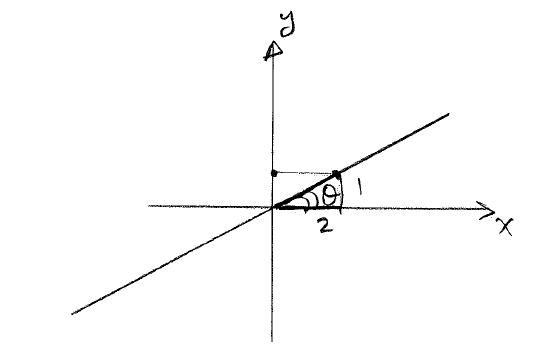
\includegraphics[height=2.25in]{3_fig7_2.jpg}}
\caption{Problem \ref{2009_a7_2}.
\label{fig_a7_2}}
\end{figure}

Note that (using Pythagoras) $\cos\theta=\frac{2}{\sqrt{5}}$, $\sin\theta=\frac{1}{\sqrt{5}}$.

Now,
$$
f\left(\left[\begin{array}{c}1\\10\end{array} \right]\right) =
\left[\begin{array}{cc}\cos(2\theta)&\sin(2\theta) \\ \sin(2\theta)&-\cos(2\theta)\end{array} \right]\left[\begin{array}{c}1\\10\end{array} \right]
$$
So, we need to calculate $\cos(2\theta)$ and $\sin(2\theta)$.

We have $\cos(2\theta) = \cos^2\theta - \sin^2\theta = \frac{4}{5}-\frac{1}{5}=\frac{3}{5}$, and $\sin(2\theta) = 2\sin\theta\cos\theta = 2\frac{2}{\sqrt{5}}\frac{1}{\sqrt{5}}=\frac{4}{5}$.

So,
$$
f\left(\left[\begin{array}{c}1\\10\end{array} \right]\right) =
\left[\begin{array}{cc}\frac{3}{5}&\frac{4}{5} \\ \frac{4}{5}&-\frac{3}{5}\end{array} \right]\left[\begin{array}{c}1\\10\end{array} \right]=\frac{1}{5}\left[\begin{array}{cc}3&4\\4&-3\end{array} \right]\left[\begin{array}{c}1\\10\end{array} \right]=\frac{1}{5}\left[\begin{array}{c}43\\-26\end{array} \right].
$$
Therefore, the matrix of $f$ is
$$
\frac{1}{5}\left[\begin{array}{cc}3&4\\4&-3\end{array}\right].
$$

%%%%%%%%%%%%%%%%%%%%%%%%%%%%%%%%%%%%%%%%%%%%%%%%%%%%%%%%%%%%%%%%%%%%%%%%%%%%%%%%
\vspace{2mm}
\noindent {\bf Solution \ref{2009_a7_3}}
Notice that $g$ is in fact the composition of $Ref_{\theta}$ and $R_{\pi/2}$, that is:
$$
g= R_{\pi/2} \circ Ref_{\theta}
$$
where $\theta$ is the angle between the line $x=-y$ and the x-axis (so, $\theta=\pi/2+\pi/4=3\pi/4$).

The matrix of $g$ is given by the product of the matrices $R_{\pi/2}$ and $Ref_{3\pi/4}$.

Note that
\begin{eqnarray*}
[g]&=&[R_{\pi/2}][Ref_{3\pi/4}]\\
&=&\left[\begin{array}{cc}\cos\pi/2&-\sin\pi/2\\ \sin\pi/2&\cos\pi/2 \end{array}\right]
\left[\begin{array}{cc}\cos6\pi/4& \sin6\pi/4\\ \sin6\pi/4&-\cos6\pi/4 \end{array}\right]\\
&=&\left[\begin{array}{cc}0&-1\\ 1&0 \end{array}\right]
\left[\begin{array}{cc}0&-1\\ -1&0 \end{array}\right]=\left[\begin{array}{cc}1&0\\ 0&-1 \end{array}\right]
\end{eqnarray*}

%%%%%%%%%%%%%%%%%%%%%%%%%%%%%%%%%%%%%%%%%%%%%%%%%%%%%%%%%%%%%%%%%%%%%%%%%%%%%%%%
\vspace{2mm}
\noindent {\bf Solution \ref{op3_12}}
Under this rotation, the vector $\eee_1=[1,0,0]$ gets transformed to
$[\cos(\theta),\sin(\theta),0]$, $\eee_2=[0,1,0]$ gets transformed to
$[-\sin(\theta),\cos(\theta),0]$, and $\eee_3=[0,0,1]$ is transformed to itself
({em i.e.} it doesn't change). Putting this in the columns of a matrix yields
\[
\left[\matrix{
\cos(\theta)&-\sin(\theta)&0\cr
\sin(\theta)&\cos(\theta)&0\cr
0&0&1\cr
}\right]
\]

%%%%%%%%%%%%%%%%%%%%%%%%%%%%%%%%%%%%%%%%%%%%%%%%%%%%%%%%%%%%%%%%%%%%%%%%%%%%%%%%
\vspace{2mm}
\noindent {\bf Solution \ref{2009_a6_5}}
Let
\begin{eqnarray*}
  \xx=(x_1,x_2,x_3,x_4)\\
	\yy=(y_1,y_2,y_3,y_4)
\end{eqnarray*}
\begin{enumerate}[1.]
\item \begin{eqnarray*}
  T(\xx+\yy)&=&T(x_1+y_1,x_2+y_2,x_3+y_3,x_4+y_4)\\
	&=&((x_1+y_1)+4(x_2+y_2)+5(x_3+y_3),3(x_1+y_1)-2(x_2+y_2)+...\\ &&(x_3+y_3)-(x_4+y_4),-(x_1+y_1)-(x_3+y_3)+(x_4+y_4))\\
	&=&(x_1+4x_2+5x_3+y_1+4y_2+5y_3,3x_1-2x_2+x_3-x_4+...\\
	&&3y_1-2y_2+y_3-y_4,-x_1-x_3+x_4-y_1-y_3+y_4)\\
	&=&(x_1+4x_2+5x_3,3x_1-2x_2+x_3-x_4,-x_1-x_3+x_4)+...\\
	&&(y_1+4y_2+5y_3,3y_1-2y_2+y_3-y_4,-y_1-y_3+y_4)\\
	&=& T(\xx)+T(\yy).
      \end{eqnarray*}
This holds for any $\xx,\yy\in\mathbb{R}^4$
\item \begin{eqnarray*}
  T(c\xx)&=&T(cx_1,cx_2,cx_3,cx_4)\\
	&=&(cx_1+4cx_2+5cx_3,3cx_1-2cx_2+cx_3-cx_4,-cx_1-cx_3+cx_4)\\
	&=&(c(x_1+4x_2+5x_3),c(3x_1-2x_2+x_3-x_4),c(-x_1-x_3+x_4))\\
	&=&c(x_1+4x_2+5x_3,3x_1-2x_2+x_3-x_4,-x_1-x_3+x_4)\\
	&=&cT(\xx).
      \end{eqnarray*}
This holds for any $\xx\in\mathbb{R}^4$, and any $c\in\mathbb{R}$. It is clear then that $T$ is linear.
\end{enumerate}

%%%%%%%%%%%%%%%%%%%%%%%%%%%%%%%%%%%%%%%%%%%%%%%%%%%%%%%%%%%%%%%%%%%%%%%%%%%%%%%%
\vspace{2mm}
\noindent {\bf Solution \ref{2009_a7_1}}
First recall the definition: a vector $\yy=(y_1,y_2,y_3)$ is said to be in the range of $T$ if there exists a vector $\xx=(x_1,x_2)$ such that $T(\xx)=\yy$.

\begin{enumerate}[a)]
  \item We should be looking for $\xx=(x_1,x_2)$, if any, such that $T(\xx)=(1,4,2)$. But
$$
\left[\begin{array}{c}1\\4\\2\end{array}\right] =
T\left(\left[\begin{array}{c}x_1\\x_2\end{array}\right]\right) =
A\left[\begin{array}{c}x_1\\x_2\end{array}\right] =
\left[\begin{array}{cc}1&2\\0&1\\1&1\end{array}\right]\left[\begin{array}{c}x_1\\x_2\end{array}\right]=\left[\begin{array}{c}x_1+2x_2\\x_2\\x_1+x_2\end{array}\right].
$$
We get the following system of equations:
$$
\left\{\begin{array}{c}x_1+2x_2=1\\x_2=4\\x_1+x_2=2\end{array}\right.\Rightarrow
\left\{\begin{array}{c}x_1+8=1\\x_1+4=2\end{array}\right.\Rightarrow
\left\{\begin{array}{c}x_1=-7\\x_1=-2\end{array}\right.
$$
So, the system does not have any solutions.

In other words, there is no $\xx=(x_1,x_2)$ that satisfy the system above. So there is no $\xx$ such that $T(\xx)=(1,4,2)$. Hence, $(1,4,2)$ is not in the range of $T$.
	\item We are looking for $\xx=(x_1,x_2)$, if any, such that $T(\xx)=(1,1,1)$.
So
$$
\left[\begin{array}{c}1\\1\\1\end{array}\right] =
T\left(\left[\begin{array}{c}x_1\\x_2\end{array}\right]\right) =
A\left[\begin{array}{c}x_1\\x_2\end{array}\right] =
\left[\begin{array}{cc}1&2\\0&1\\1&1\end{array}\right]\left[\begin{array}{c}x_1\\x_2\end{array}\right]=\left[\begin{array}{c}x_1+2x_2\\x_2\\x_1+x_2\end{array}\right].
$$
We get the following system of equations:
$$
\left\{\begin{array}{c}x_1+2x_2=1\\x_2=1\\x_1+x_2=1\end{array}\right.\Rightarrow
\left\{\begin{array}{c}x_1+2=1\\x_1+1=2\end{array}\right.\Rightarrow
\left\{\begin{array}{c}x_1=-1\\x_1=0\end{array}\right.
$$
So, as in the previous case, the system does not have any solutions; in other words, $(1,1,1)$ is not in the range of $T$.
\end{enumerate}



%%%%%%%%%%%%%%%%%%%%%%%%%%%%%%%%%%%%%%%%%%%%%%%%%%%%%%%%%%%%%%%%%%%%%%%%%%%%%%%%
\vspace{2mm}
\noindent {\bf Solution \ref{2009_a7_4}}
\begin{enumerate}[a)]
	\item Note that
$$
\left[\begin{array}{c}1\\2\\3\end{array}\right] = 
3\left[\begin{array}{c}1\\0\\0\end{array}\right]
-2\left[\begin{array}{c}1\\-1\\0\end{array}\right]
+3\left[\begin{array}{c}0\\0\\1\end{array}\right].
$$
So,
\begin{eqnarray*}
T\left(\left[\begin{array}{c}1\\2\\3\end{array}\right]\right) &=&
3T\left(\left[\begin{array}{c}1\\0\\0\end{array}\right]\right)
-2T\left(\left[\begin{array}{c}1\\-1\\0\end{array}\right]\right)
+3T\left(\left[\begin{array}{c}0\\0\\1\end{array}\right]\right)\\
&=& 3\left[\begin{array}{c}1\\1\end{array}\right]
-2\left[\begin{array}{c}2\\0\end{array}\right]
+3\left[\begin{array}{c}-1\\5\end{array}\right] =
\left[\begin{array}{c}-4\\18\end{array}\right]
\end{eqnarray*}
	\item In order to write the matrix of $T$, we need to find $T(0,1,0)$. Note that
$$
\left[\begin{array}{c}0\\1\\0\end{array}\right] =
\left[\begin{array}{c}1\\0\\0\end{array}\right]
-\left[\begin{array}{c}1\\-1\\0\end{array}\right].
$$
So, 
\begin{eqnarray*}
T\left(\left[\begin{array}{c}0\\1\\0\end{array}\right]\right) &=&
T\left(\left[\begin{array}{c}1\\0\\0\end{array}\right]\right)
-T\left(\left[\begin{array}{c}1\\-1\\0\end{array}\right]\right)\\
&=& \left[\begin{array}{c}1\\1\end{array}\right]
-\left[\begin{array}{c}2\\0\end{array}\right] =
\left[\begin{array}{c}-1\\1\end{array}\right].
\end{eqnarray*}
Now, the matrix of $T$ is given by
$$
T = \left[T\left(\left[\begin{array}{c}1\\0\\0\end{array}\right]\right)\hspace{5pt}
T\left(\left[\begin{array}{c}0\\1\\0\end{array}\right]\right)\hspace{5pt}
T\left(\left[\begin{array}{c}0\\0\\1\end{array}\right]\right)\right] =
\left[\begin{array}{ccc}1&-1&-1\\1&1&5\end{array}\right]
$$
\end{enumerate}
%%%%%%%%%%%%%%%%%%%%%%%%%%%%%%%%%%%%%%%%%%%%%%%%%%%%%%%%%%%%%%%%%%%%%%%%%%%%%%%%
\vspace{2mm}
\noindent {\bf Solution \ref{2009_a7_5}}
\begin{enumerate}[a)]
	\item
\begin{eqnarray}
  (h\circ g)\left[\begin{array}{c}1\\0\\-5\end{array}\right] &=&
	h\left(g\left[\begin{array}{c}1\\0\\-5\end{array}\right] \right) =
	h\left(\left[\begin{array}{c}1+5+0\\-5-2\times0\end{array}\right] \right)\\
	&=& h\left[\begin{array}{c}6\\-5\end{array}\right] =
	\left[\begin{array}{c}6\\-6\\-5\\5\end{array}\right].
\end{eqnarray}
\item We first find the matrix of $g$. To do so, we need to know $g(1,0,0)$, $g(0,1,0)$, and $g(0,0,1)$.

We have that
$$
g\left[\begin{array}{c}1\\0\\0\end{array}\right]=\left[\begin{array}{c}1\\0\end{array}\right],\qquad
g\left[\begin{array}{c}0\\1\\0\end{array}\right]=\left[\begin{array}{c}1\\-2\end{array}\right],\qquad
g\left[\begin{array}{c}0\\0\\1\end{array}\right]=\left[\begin{array}{c}-1\\1\end{array}\right],\qquad.
$$
So, the matrix of $g$ is
$$g = \left[\begin{array}{ccc}1&1&-1\\0&-2&1\end{array}\right].$$
Now we find the matrix of $h$. As with $g$, we need to find $h(1,0)$, and $h(0,1)$. We have that
$$
h\left[\begin{array}{c}1\\0\end{array}\right]=\left[\begin{array}{c}1\\-1\\0\\0\end{array}\right],\qquad h\left[\begin{array}{c}0\\1\end{array}\right]=\left[\begin{array}{c}0\\0\\1\\-1\end{array}\right].
$$
So, the matrix of $h$ is
$$h = \left[\begin{array}{cc}1&0\\-1&0\\0&1\\0&-1\end{array}\right].$$
\item
The matrix of $h\circ g$ is given by
$$
h\circ g = [h]_{4\times 2}[g]_{2\times3} =
\left[\begin{array}{cc}1&0\\-1&0\\0&1\\0&-1\end{array}\right]
\left[\begin{array}{ccc}1&1&-1\\0&-2&1\end{array}\right] =
\left[\begin{array}{ccc}1&1&-1\\-1&-1&1\\0&-2&1\\0&2&-1\end{array}\right]_{4\times3}
$$
We can confirm them that $h\circ g:\mathbb R^3\rightarrow\mathbb R^4$. So, the matrix of $h\circ g$ will have 4 rows and 3 columns, as expected.
\end{enumerate}

%%%%%%%%%%%%%%%%%%%%%%%%%%%%%%%%%%%%%%%%%%%%%%%%%%%%%%%%%%%%%%%%%%%%%%%%%%%%%%%%
\vspace{2mm}
\noindent {\bf Solution \ref{op3_13}}
We can determine the transition matrix, since we know each $p_{i,i}=0$, and the sum over each
column is one. We are given that $p_{2,1}=1/2$. Then, since $p_{1,1}+p_{2,1}+p_{3,1}=1$, we
have $0+1/2+p_{3,1}=1$, so $p_{3,1}=1/2$. Similarly $p_{1,2}=1/3$, $p_{3,2}=2/3$, 
and $p_{1,3}=1/4$, $p_{2,3}=3/4$. Thus
\[
P=\left[\matrix{0&1/3&1/4\cr 1/2&0&3/4\cr 1/2&2/3&0\cr}\right]
\]
If we start out with the probability vector $\xx_0=\left[\matrix{1\cr 0\cr 0\cr}\right]$ (i.e., the walker
is in location $1$) then after two time steps the probability vector is $P^2\xx_0$, i.e.,
\[
\xx_2=\left[\matrix{7/24&1/6&1/4\cr 3/8&2/3&1/8\cr 1/3&1/6&5/8\cr}\right]
\left[\matrix{1\cr 0\cr 0\cr}\right]=\left[\matrix{7/24\cr 3/8\cr 1/3\cr}\right]
\]
So the probability that the walker is in position $2$ after two time steps is $3/8$.

%%%%%%%%%%%%%%%%%%%%%%%%%%%%%%%%%%%%%%%%%%%%%%%%%%%%%%%%%%%%%%%%%%%%%%%%%%%%%%%%
\vspace{2mm}
\noindent {\bf Solution \ref{2009_a8_3}}
\begin{enumerate}[a)]
  \item Since $P_{i,i}=0$, and the sum of entries in each column is 1, the matrix $P$ is
$$
P=\left[\begin{array}{ccc}0&2/5&1/4\\1/3&0&3/4\\2/3&3/5&0\end{array}\right].
$$
	\item The random walker starts at location 1. So $\xx_0=(1,0,0)^T$. The positions after three time steps will be
$$
\xx_1=P\xx_0=\left[\begin{array}{c}0\\1/3\\2/3\end{array}\right],\qquad
\xx_2=P\xx_1=\left[\begin{array}{c}3/10\\1/2\\1/5\end{array}\right],\qquad
\xx_3=P\xx_2=\left[\begin{array}{c}1/4\\1/4\\1/2\end{array}\right],\qquad
$$
So, $\xx_{3,2}$, that is, the probability that the random walker is in location 2 after 3 steps, will be $\frac{1}{4}=0.25$.
	\item
$$
\xx_0=\left[\begin{array}{c}0\\0\\1\end{array}\right],\qquad
\xx_1=P\xx_0=\left[\begin{array}{c}1/4\\3/4\\0\end{array}\right],\qquad
\xx_2=P\xx_1=\frac{1}{60}\left[\begin{array}{c}18\\5\\37\end{array}\right],\qquad
$$
So, $\xx_{2,1}$, the probability that the random walker is in location 1 after 2 steps, will be $\frac{18}{60}=0.333..$.
\end{enumerate}
%%%%%%%%%%%%%%%%%%%%%%%%%%%%%%%%%%%%%%%%%%%%%%%%%%%%%%%%%%%%%%%%%%%%%%%%%%%%%%%%
\vspace{2mm}
\noindent {\bf Solution \ref{2009_a8_4}}
\begin{enumerate}[a)]
  \item
\begin{eqnarray}
  &&P\left[\begin{array}{cccc}1/4&1/4&1/4&1/4\\1/4&1/4&1/4&1/4\\1/4&1/4&1/4&1/4\\1/4&1/4&1/4&1/4\end{array}\right] =
	\frac{1}{4}\left[\begin{array}{cccc}1&1&1&1\\1&1&1&1\\1&1&1&1\\1&1&1&1\end{array}\right]\\
	&&P^2=\frac{1}{4}\frac{1}{4}\left[\begin{array}{cccc}4&4&4&4\\4&4&4&4\\4&4&4&4\\4&4&4&4\end{array}\right]=
	\frac{1}{4\cdot4}\cdot4\left[\begin{array}{cccc}1&1&1&1\\1&1&1&1\\1&1&1&1\\1&1&1&1\end{array}\right].
\end{eqnarray}
So, $P^2=P$, thus $P^3=P\cdot P^2=P\cdot P=P$. Hence, $P^n=P$ for every $n\ge1$
\item
Let
$$
\xx_0=\left[\begin{array}{c}1\\0\\0\\0\end{array}\right].
$$
Then 
$$
\xx_1=\frac{1}{4}\left[\begin{array}{c}1\\1\\1\\1\end{array}\right].
$$
Hence, $\xx_n=P^n\xx_0$. But $P^n=P$, for every $n\ge1$. So,
$$
\xx_n = P^n\xx_0=P\xx_0=\xx_1=
\frac{1}{4}\left[\begin{array}{c}1\\1\\1\\1\end{array}\right].
$$
\end{enumerate}
Now, let
$$
\xx_0=\left[\begin{array}{c}0\\0\\0\\1\end{array}\right],\qquad
\xx_1=P\xx_0=\frac{1}{4}\left[\begin{array}{c}1\\1\\1\\1\end{array}\right].
$$
Again
$$
\xx_n = P^n\xx_0=P\xx_0=
\frac{1}{4}\left[\begin{array}{c}1\\1\\1\\1\end{array}\right].
$$

%%%%%%%%%%%%%%%%%%%%%%%%%%%%%%%%%%%%%%%%%%%%%%%%%%%%%%%%%%%%%%%%%%%%%%%%%%%%%%%%
\vspace{2mm}
\noindent {\bf Solution \ref{2009_a8_5}}
$$
P=\left[\begin{array}{ccc}1/3&1/4&2/5\\0&1/2&1/5\\2/3&1/4&2/5\end{array} \right]
$$
\begin{enumerate}[a)]
  \item We are given
$$
x_0=\left[\begin{array}{c}0\\1\\0\end{array}\right].
$$
Then
$$
\xx_1=P\xx_0=\left[\begin{array}{c}1/4\\1/2\\1/4\end{array}\right].
$$
So, $x_{1,1}=\frac{1}{4}$ is the probability that the random walker is location 1 after one time step.
	\item
Again
$$
x_0=\left[\begin{array}{c}0\\1\\0\end{array}\right].
$$
Then
$$
\xx_1=P\xx_0=\left[\begin{array}{c}1/4\\1/2\\1/4\end{array}\right],\qquad
\xx_2=P\xx_1=\left[\begin{array}{c}\frac{37}{120}\\\frac{3}{10}\\\frac{47}{120}\end{array}\right]\qquad\Rightarrow\qquad
\xx_{2,1}=\frac{37}{120}.
$$
	\item
$$
\xx_0=\left[\begin{array}{c}1/3\\1/3\\1/3\end{array}\right].
$$
We have
\begin{eqnarray*}
\xx_1=P\xx_0=\left[\begin{array}{c}\frac{59}{180}\\\frac{7}{30}\\\frac{79}{180}\end{array}\right],\qquad
\xx_2=P\xx_1=\left[\begin{array}{c}\frac{1853}{5400}\\ \frac{46}{225}\\ \frac{2443}{5400}\end{array}\right]
\end{eqnarray*}
Therefore, $\xx_{2,3}=\frac{2443}{5400}$
\end{enumerate}

%%%%%%%%%%%%%%%%%%%%%%%%%%%%%%%%%%%%%%%%%%%%%%%%%%%%%%%%%%%%%%%%%%%%%%%%%%%%%%%%
\vspace{2mm}
\noindent {\bf Solution \ref{op3_14}}
In this situation the transition matrix is
\[
P={{1}\over{3}}\left[\matrix{1&1&1\cr 1&1&1\cr 1&1&1\cr}\right]
\]
so
$P=P^2=p^3=\cdots P^n$. In this case, if we start out with any probability vector 
$\xx_0=\left[\matrix{x_1&x_2&x_3cr}\right]$ with $x_1+x_2+x_3=1$, then
\[
P\xx_0 = \left[\matrix{1/3\cr1/3\cr1/3\cr}\right]=P^n\xx_0
\]
for each $n$.

%%%%%%%%%%%%%%%%%%%%%%%%%%%%%%%%%%%%%%%%%%%%%%%%%%%%%%%%%%%%%%%%%%%%%%%%%%%%%%%%
\vspace{2mm}
\noindent {\bf Solution \ref{newp4_1}}
\begin{enumerate}[(a)]
\item The transition matrix is 
\[
P = \left[ \begin{array}{ccc}
1/2 & 0 & 1/3 \\ 1/4 & 1/2 & 1/3 \\ 1/4 & 1/2 & 1/3 
\end{array} \right]
\]
The system starts in state 3 so $\xx^{(0)} = \eee_3$. After one step, 
the probability vector is 
\[
\xx^{(1)} = P \xx^{(0)} = 
\left[ \begin{array}{ccc}
1/2 & 0 & 1/3 \\ 1/4 & 1/2 & 1/3 \\ 1/4 & 1/2 & 1/3 
\end{array} \right]
\threevec{0}{0}{1} = \threevec{1/3}{1/3}{1/3} 
\]
That is, there is a equal probability of being in any state. 
After another step, 
\[
\xx^{(2)} = P \xx^{(1)} = 
\left[ \begin{array}{ccc}
1/2 & 0 & 1/3 \\ 1/4 & 1/2 & 1/3 \\ 1/4 & 1/2 & 1/3 
\end{array} \right]
\threevec{1/3}{1/3}{1/3} = \threevec{5/18}{13/36}{13/36} 
\]
So the probability that the system is in state 2 is 13/36. 
\item Suppose that the initial probabilities are given by the vector 
\[
\xx^{(0)} = \threevec{x_1}{x_2}{x_3}.
\]
Then after $k$ steps, the probabilities will be 
$\xx^{(k)} = P^k \xx^{(0)}$. After many steps (using the limiting 
behaviour of $P^k$ stated in the question):
\begin{eqnarray*}
\xx^{(k)} & \approx & 
 \left[ \begin{array}{ccc}
0.25 & 0.25 & 0.25 \\ 0.375 & 0.375 & 0.375 \\ 0.375 & 0.375 & 0.375
\end{array} \right]
\threevec{x_1}{x_2}{x_3} \\
  & = & 
 \left[ \begin{array}{c}
0.25 x_1+  0.25 x_2+  0.25 x_3\\ 
0.375 x_1+  0.375 x_2+  0.375 x_3\\ 
0.375 x_1+ 0.375 x_2+ 0.375 x_3
\end{array} \right] \\
  & = & (x_1+x_2+x_3) \threevec{0.25}{0.375}{0.375} \\
  & = & \threevec{0.25}{0.375}{0.375} 
\end{eqnarray*}
where the last line follows because the initial probabilities must sum 
to one. Note that the state tends to this probability distribution no 
matter what the initial state is (or initial probabilities are). This 
is known as the steady state probability vector of this random walk. 
\end{enumerate}

%%%%%%%%%%%%%%%%%%%%%%%%%%%%%%%%%%%%%%%%%%%%%%%%%%%%%%%%%%%%%%%%%%%%%%%%%%%%%%%%
\vspace{2mm}
\noindent {\bf Solution \ref{op3_15}}
\[
A\xx = \left[
\begin{array}{c} x_1+2x_2+3x_3 \\ 4x_1+5x_2+6x_3 \end{array} \right]
\]
so $\yy\cdot A\xx =
y_1x_1+2y_1x_2+3y_1x_3+4y_2x_1+5y_2x_2+6y_2x_3$. On the other hand
\[
A^T\yy = \left[ \begin{array}{c}
y_1+4y_2 \\ 2y_1+5y_2 \\ 3y_1+6y_2 
\end{array} \right]
\]
so
$(A^T\yy)\cdot \xx = y_1x_1+4y_2x_1+2y_1x_2+5y_2x_2+3y_1x_3+6y_2x_3$.
These expressions are equal.

%%%%%%%%%%%%%%%%%%%%%%%%%%%%%%%%%%%%%%%%%%%%%%%%%%%%%%%%%%%%%%%%%%%%%%%%%%%%%%%%
\vspace{2mm}
\noindent {\bf Solution \ref{op3_16}}
$(A^T)^T=A$.

%%%%%%%%%%%%%%%%%%%%%%%%%%%%%%%%%%%%%%%%%%%%%%%%%%%%%%%%%%%%%%%%%%%%%%%%%%%%%%%%
\vspace{2mm}
\noindent {\bf Solution \ref{op3_17}}
$AB=\twovec{9&12&15}{7&11&15}$ so $(AB)^T=\threevec{9&7}{12&11}{15&15}$.
On the other hand $B^TA^T = \threevec{1&4}{2&5}{3&6}\twovec{1&3}{2&1}
=\threevec{9&7}{12&11}{15&15}$.

%%%%%%%%%%%%%%%%%%%%%%%%%%%%%%%%%%%%%%%%%%%%%%%%%%%%%%%%%%%%%%%%%%%%%%%%%%%%%%%%
\vspace{2mm}
\noindent {\bf Solution \ref{op3_18}}
If $\yy=\eee_i$ and $\xx=\eee_j$ (vectors that are all zeros except in
one spot) then $\yy\cdot (A\xx)= \eee_i\cdot (A\eee_j)$ is the matrix
entry $a_{i j}$. So we can conclude that all the matrix entries of $A$ are
the same as those for $B$. This means the matrices must be the same.

%%%%%%%%%%%%%%%%%%%%%%%%%%%%%%%%%%%%%%%%%%%%%%%%%%%%%%%%%%%%%%%%%%%%%%%%%%%%%%%%
\vspace{2mm}
\noindent {\bf Solution \ref{op3_19}}
$\xx\cdot(A\yy) = \xx^T A\yy = (A^T\xx)^T\yy = (A^T\xx)\cdot\yy$

%%%%%%%%%%%%%%%%%%%%%%%%%%%%%%%%%%%%%%%%%%%%%%%%%%%%%%%%%%%%%%%%%%%%%%%%%%%%%%%%
\vspace{2mm}
\noindent {\bf Solution \ref{op3_22}}
To determine whether these matrices invertible we reduce them using Gaussian
elimination. This gives
\begin{enumerate}[(a)]
\item $\left[\matrix{1&2\cr0&-2\cr}\right]$
\item $\left[\matrix{1&2&3\cr0&3&4\cr0&0&-1/3\cr}\right]$
\item $\left[\matrix{1&2&3\cr0&3&4\cr0&0&2/3\cr}\right]$
\end{enumerate}
Since these all have rank equal to their size, they are all invertible.

%%%%%%%%%%%%%%%%%%%%%%%%%%%%%%%%%%%%%%%%%%%%%%%%%%%%%%%%%%%%%%%%%%%%%%%%%%%%%%%%
\vspace{2mm}
\noindent {\bf Solution \ref{op3_23}}
The inverse is
\[
\left[\matrix{-5&2\cr3&-1\cr}\right]
\]

%%%%%%%%%%%%%%%%%%%%%%%%%%%%%%%%%%%%%%%%%%%%%%%%%%%%%%%%%%%%%%%%%%%%%%%%%%%%%%%%
\vspace{2mm}
\noindent {\bf Solution \ref{op3_24}}
\begin{enumerate}[(a)]
\item This matrix reduces to 
$\left[\matrix{2&3&-1\cr0&1/2&7/2\cr0&0&0\cr}\right]$ and so is not invertible
\item The inverse is  $\left[\matrix{-1&0&1\cr1&1&0\cr3&1&-1\cr}\right]$
\item $\left[\matrix{3&-5/2&1/2\cr-3&4&-1\cr1&-3/2&1/2\cr}\right]$
\item $\left[\matrix{-7&5&3\cr3&-2&-2\cr3&-2&-1\cr}\right]$
\item $\left[\matrix{1&0&-a\cr0&1&0\cr0&0&1\cr}\right]$
\item $\left[\matrix{1&-a&ac-b\cr0&1&-c\cr0&0&1\cr}\right]$
\end{enumerate}

%%%%%%%%%%%%%%%%%%%%%%%%%%%%%%%%%%%%%%%%%%%%%%%%%%%%%%%%%%%%%%%%%%%%%%%%%%%%%%%%
\vspace{2mm}
\noindent {\bf Solution \ref{2009_a8_1}}
In order to find the inverse of $A$, we form the augmented matrix $[A|I]$. Then we apply elementary row operations to $A$, to reduce $A$ to its rref-form. If A is invertible, then using this method $[A|I]$ transfers to $[I|B]$, where $B$ is the inverse of $A$.

Now, let
$$A = \left[\begin{array}{ccc}1&1&1\\0&2&3\\5&5&1\end{array}\right]$$
and form the augmented matrix:
$$
\left[\begin{array}{ccc|ccc}1&1&1&1&0&0\\0&2&3&0&1&0\\5&5&1&0&0&1\end{array}\right]
$$
The reduced row echelon form of the augmented matrix is
$$
\left[\begin{array}{ccc|ccc}1&0&0&13/8&-1/2&-1/8 \\ 0&1&0&-15/8&1/2&3/8 \\ 0&0&1&5/4&0&-1/4 \end{array}\right]
$$
Therefore, the inverse of $A$ is
$$
A^{-1} = \left[\begin{array}{ccc}13/8&-1/2&-1/8 \\ -15/8&1/2&3/8 \\ 5/4&0&-1/4 \end{array}\right].
$$

Let
$$B = \left[\begin{array}{cccc}1&2&-3&1\\-1&3&-3&-2\\2&0&1&5\\3&1&-2&5\end{array}\right]$$
Applying the same method, we observe that $B$ is not invertible because
$$
rref(B) = \left[\begin{array}{cccc}1&0&0&2\\0&1&0&1\\0&0&1&1\\0&0&0&0\end{array}\right].
$$
Note that rank of $B=3$, which is the number of non-zero rows in rref($B$).

%%%%%%%%%%%%%%%%%%%%%%%%%%%%%%%%%%%%%%%%%%%%%%%%%%%%%%%%%%%%%%%%%%%%%%%%%%%%%%%%
\vspace{2mm}
\noindent {\bf Solution \ref{2009_a8_2}}
\begin{enumerate}[a)]
  \item Let
$$
A = \left[\begin{array}{ccc}1&0&5\\1&-2&3\\2&1&-3\end{array}\right]
$$
be the coefficient matrix. Then
$$
A\xx = \left[\begin{array}{c}6\\14\\-2\end{array}\right]
$$
	\item
$$
A^{-1} = \left[\begin{array}{ccc}3/28&5/28&5/14\\9/28&-13/28&1/14\\5/28&-1/28&-1/14\end{array}\right]
=\frac{1}{28}\left[\begin{array}{ccc}3&5&10\\9&-13&2\\5&-1&-2\end{array}\right]
$$
	\item
In order to solve the system $A\xx=\bb$, we multiply both sides by $A^{-1}$:
\begin{eqnarray*}
  &&A^{-1}A\xx=A^{-1}\bb=A^{-1}\left[\begin{array}{c}6\\14\\-2\end{array}\right]=
	\frac{1}{7}\left[\begin{array}{c}17\\-33\\5\end{array}\right]\\
	&&\Rightarrow \qquad I\xx=\xx=\left[\begin{array}{c}17\\-33\\5\end{array}\right].
\end{eqnarray*}
So, the system has the \textbf{unique} solution
$$
\xx=\left[\begin{array}{c}17\\-33\\5\end{array}\right]
$$
\end{enumerate}

%%%%%%%%%%%%%%%%%%%%%%%%%%%%%%%%%%%%%%%%%%%%%%%%%%%%%%%%%%%%%%%%%%%%%%%%%%%%%%%%
\vspace{2mm}
\noindent {\bf Solution \ref{op3_27}}
We reduce the matrix as follows:
\[
\left[\matrix{1&1&1&1\cr 1&2&4&8\cr 1&3&9&27\cr 1&4&16&64\cr}\right]
\]
\[
\left[\matrix{1&1&1&1\cr 0&1&3&7\cr 0&2&8&26\cr 0&3&15&63\cr}\right]
\matrix{\cr (R2)-(R1)\cr (R3)-(R1)\cr  (R4)-(R1)\cr}
\]
\[
\left[\matrix{1&1&1&1\cr 0&1&3&7\cr 0&0&2&12\cr 0&0&6&42\cr}\right]
\matrix{\cr\cr(R3)-2(R2)\cr (R4)-3(R2)\cr}
\]
\[
\left[\matrix{1&1&1&1\cr 0&1&3&7\cr 0&0&2&12\cr 0&0&0&6\cr}\right]
\matrix{\cr\cr\cr (R4)-3(R3)\cr}
\]
None of these operations affect the determinant. So the determinant of the
original matrix is the same as the determinant of the reduced diagonal matrix.
This determinant is the product of the diagonal elements which equals $12$.

%%%%%%%%%%%%%%%%%%%%%%%%%%%%%%%%%%%%%%%%%%%%%%%%%%%%%%%%%%%%%%%%%%%%%%%%%%%%%%%%
\vspace{2mm}
\noindent {\bf Solution \ref{op3_28}}
We reduce the matrix as follows:
\[
\left[\matrix{1&-1&1&-1\cr 1&2&4&8\cr 1&-2&4&-8\cr 1&1&1&1\cr}\right]
\]
\[
\left[\matrix{1&-1&1&-1\cr 0&3&3&9\cr 0&-1&3&-7\cr 0&2&0&2\cr}\right]
\matrix{\cr (R2)-(R1)\cr (R3)-(R1)\cr  (R4)-(R1)\cr}
\]
\[
\left[\matrix{1&-1&1&-1\cr 0&1&1&3\cr 0&-1&3&-7\cr 0&2&0&2\cr}\right]
\matrix{\cr (1/3)(R2)\cr\cr\cr}
\]
\[
\left[\matrix{1&-1&1&-1\cr 0&1&1&3\cr 0&0&4&-4\cr 0&0&-2&-4\cr}\right]
\matrix{\cr\cr(R3)+(R2)\cr(R4)-2(R2)\cr}
\]
\[
\left[\matrix{1&-1&1&-1\cr 0&1&1&3\cr 0&0&1&-1\cr 0&0&-2&-4\cr}\right]
\matrix{\cr\cr(1/4)(R3)\cr\cr}
\]
\[
\left[\matrix{1&-1&1&-1\cr 0&1&1&3\cr 0&0&1&-1\cr 0&0&0&-6\cr}\right]
\matrix{\cr\cr\cr(R4)+2(R3)\cr}
\]
The two operations that changed the determinant were multiplying the 
the second row by $1/3$ and multiplying the third row by $1/4$. Thus
the determinant of the diagonal matrix is $(1/3)(1/4)\times$ the determinant
of the original matrix. Hence the determinant of the original matrix
is $3\times 4\times (-6)= -72$.

%%%%%%%%%%%%%%%%%%%%%%%%%%%%%%%%%%%%%%%%%%%%%%%%%%%%%%%%%%%%%%%%%%%%%%%%%%%%%%%%
\vspace{2mm}
\noindent {\bf Solution \ref{2009_a9_1}}
\begin{enumerate}[a)]
  \item
\begin{eqnarray*}
  \det A&=&\det\left[\begin{array}{cccc}2&0&2&4\\0&0&3&2\\2&2&4&4\\3&0&6&2\end{array}\right]\\
	&=&2\det\left[\begin{array}{ccc}0&3&2\\2&4&4\\0&6&2\end{array}\right]-0
	+2\det\left[\begin{array}{ccc}0&0&2\\2&2&4\\3&0&2\end{array}\right]
	-4\det\left[\begin{array}{ccc}0&0&3\\2&2&4\\3&0&6\end{array}\right]\\
	&=&2\left(0-3\det\left[\begin{array}{cc}2&4\\0&2\end{array}\right]
	+2\det\left[\begin{array}{cc}2&4\\0&6\end{array}\right]\right)
	+2(2)\det\left[\begin{array}{cc}2&2\\3&0\end{array}\right]-\cdots\\
	&&\qquad4(3)\det\left[\begin{array}{cc}2&2\\3&0\end{array}\right]\\
	&=&2(0-3(4-0)+2((2-0))+4(0-6)-12(0-6)\\
	&=&2(12)-24+72=\bf72.
\end{eqnarray*}
\item
\begin{eqnarray*}
  \det A&=&\det\left[\begin{array}{cccc}2&0&2&4\\0&0&3&2\\2&2&4&4\\3&0&6&2\end{array}\right]\\
	&=&-0+0-2\det\left[\begin{array}{ccc}2&2&4\\0&3&2\\3&6&2\end{array}\right]+0\\
	&=&-2\left(-0+3\det\left[\begin{array}{cc}2&4\\3&2\end{array}\right]
	-2\det\left[\begin{array}{cc}2&2\\3&6\end{array}\right]\right)\\
	&=&-2(3(4-12)-2(12-6))\\
	&=&-2(-24-12)=\bf72
\end{eqnarray*}
\end{enumerate}

%%%%%%%%%%%%%%%%%%%%%%%%%%%%%%%%%%%%%%%%%%%%%%%%%%%%%%%%%%%%%%%%%%%%%%%%%%%%%%%%
\vspace{2mm}
\noindent {\bf Solution \ref{op3_29}}
\begin{eqnarray*}
\det\left[\matrix{1&0&1\cr 1&2&3\cr 3&0&1\cr}\right]
&=&-1\det\left[\matrix{0&1\cr0&1}\right]
+2\det\left[\matrix{1&1\cr 3&1}\right] 
-3\det\left[\matrix{1&0\cr 3&0}\right]\\
&=& -1\times 0 +2\times(1-3) -3\times 0
= -4 \\
\det\left[\matrix{1&0&1\cr 1&2&3\cr 3&0&1\cr}\right]
&=&1\det\left[\matrix{1&2\cr3&0}\right]
-3\det\left[\matrix{1&0\cr3&0}\right]
+1\det\left[\matrix{1&0\cr1&2}\right]\\
&=&1\times(0-6) -3\times 0 + 1\times(2-0) = -4
\end{eqnarray*}

%%%%%%%%%%%%%%%%%%%%%%%%%%%%%%%%%%%%%%%%%%%%%%%%%%%%%%%%%%%%%%%%%%%%%%%%%%%%%%%%
\vspace{2mm}
\noindent {\bf Solution \ref{2009_a9_2}}
\begin{eqnarray*}
  D&=&\det\left[\begin{array}{cccc}2&0&2&4\\0&0&3&2\\2&2&4&4\\3&0&6&2\end{array}\right]
	\qquad\rarr\qquad(1,:)=\frac{1}{2}(1,:)\\
	\frac{1}{2}D&=&\det\left[\begin{array}{cccc}1&0&1&2\\0&0&3&2\\2&2&4&4\\3&0&6&2\end{array}\right]
	\qquad\rarr\qquad\begin{array}{c}(3,:)=(3,:)-2(1,:)\\(4,:)=(4,:)-3(1,:)\end{array}\\
	\frac{1}{2}D&=&\det\left[\begin{array}{cccc}1&0&1&2\\0&0&3&2\\0&2&2&0\\0&0&3&-4\end{array}\right]
	\qquad\rarr\qquad(4,:)=(4,:)-(2,:)\\
	\frac{1}{2}D&=&\det\left[\begin{array}{cccc}1&0&1&2\\0&0&3&2\\0&2&2&0\\0&0&0&-6\end{array}\right]
	\qquad\rarr\qquad(2,:)\leftrightarrow(3,:)\\
	-\frac{1}{2}D&=&\det\left[\begin{array}{cccc}1&0&1&2\\0&2&2&0\\0&0&3&2\\0&0&0&-6\end{array}\right]
\end{eqnarray*}
Therefore, $-\frac{1}{2}D=(1)(2)(3)(-6)=-36\qquad\rightarrow\qquad D=\bf72$.

%%%%%%%%%%%%%%%%%%%%%%%%%%%%%%%%%%%%%%%%%%%%%%%%%%%%%%%%%%%%%%%%%%%%%%%%%%%%%%%%
\vspace{2mm}
\noindent {\bf Solution \ref{2009_a9_3}}
If $n$ is even, then $\frac{n}{2}$ row interchanges are required to reduce the matrix to a diagonal matrix. Therefore, the determinant is $(-1)^{n/2}a_1a_2\cdots a_n$.

If $n$ is odd, then $\frac{n-1}{2}$ row interchanges are required to reduce the matrix to a diagonal matrix (note that the centre row stays). Therefore, the determinant is $(-1)^{\frac{n-1}{2}}a_1a_2\cdots a_n$.

In other words:
$$
\det\left[\begin{array}{cccc}&&&a_n\\&&\rdots\\&a_2\\a_1\end{array}\right]=
(-1)^k\det\left[\begin{array}{cccc}a_1\\&a_2\\&&\ddots\\&&&a_n\end{array}\right]=
(-1)^ka_1a_2\cdots a_n,
$$
where
$$
k=\left\{\begin{array}{c}\frac{n}{2}\qquad n\hspace{3pt}\textrm{even}\\\frac{n-1}{2}\qquad n\hspace{3pt}\textrm{odd}\end{array}\right.
$$
Alternatively, we can expand the determinant on the first row:
\begin{eqnarray*}
\det\left[\begin{array}{cccc}&&&a_n\\&&\rdots\\&a_2\\a_1\end{array}\right]&=&
(-1)^{1+n}a_n
\det\left[\begin{array}{cccc}&&&a_{n-1}\\&&\rdots\\&a_2\\a_1\end{array}\right]\\
&=&(-1)^{1+n}a_n(-1)^{1+(n-1)}a_{n-1}
\det\left[\begin{array}{cccc}&&&a_{n-2}\\&&\rdots\\&a_2\\a_1\end{array}\right]\\
&=&\cdots\\
&=&(-1)^{1+n}a_n(-1)^{1+(n-1)}a_{n-1}\cdots(-1)^{1+1}a_1\\
&=&(-1)^{(1+n)+n+\cdots+2}a_1a_2\cdots a_n\\
&=&(-1)^{\frac{(n+1)(n+2)}{2}-1}a_1a_2\cdots a_n
\end{eqnarray*}

%%%%%%%%%%%%%%%%%%%%%%%%%%%%%%%%%%%%%%%%%%%%%%%%%%%%%%%%%%%%%%%%%%%%%%%%%%%%%%%%
\vspace{2mm}
\noindent {\bf Solution \ref{2009_a9_4}}
A matrix is not invertible if and only if its determinant is equal to zero. Therefore, all we need to do is find the determinant of the matrix, and determine the values of $\lambda$ that make the determinant zero.
\begin{eqnarray*}
\det\left[\begin{array}{ccc}2-\lambda&1&0\\-1&-\lambda&1\\1&3&1-\lambda\end{array}\right] &=&
(2-\lambda)\det\left[\begin{array}{cc}-\lambda&1\\3&1-\lambda\end{array}\right] -
\det\left[\begin{array}{cc}-1&1\\1&1-\lambda\end{array}\right] + 0\\
&=&(2-\lambda)(-\lambda(1-\lambda)-3)-(-(1-\lambda)-1)\\
&=&(2-\lambda)\left(\lambda^2-\lambda-3\right)-(\lambda-2)\\
&=&(2-\lambda)(\lambda^2-\lambda-2)\\
&=&(2-\lambda)(\lambda-2)(\lambda+1)=0\\
\Rightarrow\qquad \lambda=\bf{2,-1}
\end{eqnarray*}

%%%%%%%%%%%%%%%%%%%%%%%%%%%%%%%%%%%%%%%%%%%%%%%%%%%%%%%%%%%%%%%%%%%%%%%%%%%%%%%%
\vspace{2mm}
\noindent {\bf Solution \ref{2009_a9_5}}
\begin{enumerate}[a)]
  \item \textbf{False}\qquad Counterexample:
$$
\det\left[\begin{array}{cc}1&1\\1&1\end{array}\right]=0\neq 1
$$
The correct statement should be:

The determinant of \textbf{a triangular (or diagonal) matrix} is the product of the entries of its main diagonal.
	\item \textbf{False}\qquad Counterexample:
$$
A=[1\hspace{3pt}2]\in\mathbb{R}^{1\times2}.
$$
Then
\begin{eqnarray*}
  \det(AA^T)&=&\det\left([1\hspace{3pt}2]\left[\begin{array}{c}1\\2\end{array}\right]\right)\\
	&=&\det([5])=5\\
  \det(A^TA)&=&\det\left(\left[\begin{array}{c}1\\2\end{array}\right][1\hspace{3pt}2]\right)\\
	&=&\det\left[\begin{array}{cc}1&2\\2&4\end{array}\right]=0\\
\end{eqnarray*}
Therefore, $\det(AA^T)\neq(A^TA)$.

The correct statement should be:

For \textbf{every square matrix $A$}, we have  $\det(AA^T)=(A^TA)$.
	\item \textbf{True}\qquad Since
\begin{eqnarray*}
\det(B^{-1}AB)&=&\det(B^{-1})\det(A)\det(B)=\frac{\det(A)\det(B)}{\det(B)}=\det(A)\\
\det(BAB^{-1})&=&\det(B)\det(A)\det(B^{-1})=\frac{\det(B)\det(A)}{\det(B)}=\det(A).
\end{eqnarray*}
\item \textbf{False}\qquad Counterexample: Let
$$
A=\left[\begin{array}{cc}1&0\\0&1\end{array}\right]
$$
Then
\begin{eqnarray*}
  \det(A)&=&1\\
	\det(2A)&=&\det\left[\begin{array}{cc}2&0\\0&2\end{array}\right]=4\\
	\Rightarrow\qquad\det(A)\neq2\det(A).
\end{eqnarray*}
The correct statement should be:

If an $n\times n$ matrix $A$ is multiplied by a scalar $c$, the determinant of the resulting matrix is $\bf{\det(cA)=c^n\cdot\det(A)}$.
	\item \textbf{True}\qquad Since suppose the column vectors of $A\in\mathbb{R}^{n\times n}$ are linearly independent, then $A\xx=0$ has a unique solution $\xx=\vec{0}$. The row vectors of $A^T$ will also be linearly independent, hence $A^T\xx=0$ also has a unique solution $\xx=\vec{0}$. Furthermore, since the columns are linearly independent,
	$$
	\det(A)\neq0\qquad\Rightarrow\qquad\det(A^T)=\det(A)\neq0.
$$

%%%%%%%%%%%%%%%%%%%%%%%%%%%%%%%%%%%%%%%%%%%%%%%%%%%%%%%%%%%%%%%%%%%%%%%%%%%%%%%%
\vspace{2mm}
\noindent {\bf Solution \ref{op3_20}}
$B=\threevec{1&1}{1&0}{1&1}$ and $\bb=\threevec{1}{1}{0}$ so
$B^TB = \twovec{3&2}{2&2}$ and $B^T\bb=\twovec{2}{1}$ The equation
$B^TB\xx = B^T\bb$ has solution $\xx=\twovec{1}{-1/2}$. For this
vector $\xx$ we have $B\xx = \threevec{1/2}{1}{1/2}$

%%%%%%%%%%%%%%%%%%%%%%%%%%%%%%%%%%%%%%%%%%%%%%%%%%%%%%%%%%%%%%%%%%%%%%%%%%%%%%%%
\vspace{2mm}
\noindent {\bf Solution \ref{op3_21}}
We obtain $B=\threevec{x_1&1}{x_2&1}{x_3&1}$ and $\bb=\threevec{y_1}{y_2}{y_3}$
so that $B^TB = \twovec{\sum x_i^2 & \sum x_i}{\sum x_i&n}$ (where $n=3$ in
this example) and $B^T\bb = \twovec{\sum x_i y_i}{\sum y_i}$. Thus we end up
with the same equations as before.

%%%%%%%%%%%%%%%%%%%%%%%%%%%%%%%%%%%%%%%%%%%%%%%%%%%%%%%%%%%%%%%%%%%%%%%%%%%%%%%%
\vspace{2mm}
\noindent {\bf Solution \ref{op3_25}}
The inverse operation to multiplying the first row by two is multiplying
the first row by $1/2$. Therefore the inverse elementary matrix to
$\left[\matrix{2&0&0\cr0&1&0\cr0&0&1\cr}\right]$ is 
$\left[\matrix{1/2&0&0\cr0&1&0\cr0&0&1\cr}\right]$. 

The inverse operation to subtracting twice the first row from the second row is
adding twice the first row to the second row. Therefore the inverse elementary matrix to
$\left[\matrix{1&0&0\cr-2&1&0\cr0&0&1\cr}\right]$ is 
$\left[\matrix{1&0&0\cr2&1&0\cr0&0&1\cr}\right]$.

The inverse operation to exchanging the last two rows is exchanging them again. 
Therefore the inverse elementary matrix to
$\left[\matrix{1&0&0\cr0&0&1\cr0&1&0\cr}\right]$ is the same matrix
$\left[\matrix{1&0&0\cr0&0&1\cr0&1&0\cr}\right]$.

In each case one can check directly that the inverse matrices when multiplied
by the original matrices give the identity matrix.

%%%%%%%%%%%%%%%%%%%%%%%%%%%%%%%%%%%%%%%%%%%%%%%%%%%%%%%%%%%%%%%%%%%%%%%%%%%%%%%%
\vspace{2mm}
\noindent {\bf Solution \ref{op3_26}}
We can reduce $A$ to the identity with the following row operations:
$(R2) - (1/2)(R1)$, $(R3) + (1/2)(R1)$, $(R3) - (R2)$, $(R1) - 6(R2)$, 
$(R2)-(5/4)(R3)$, $(R1) + 7(R3)$, $(1/2)(R1)$, $2(R2)$, $(1/2)(R3)$.
So
\[ {\tiny 
\threevec{1&0&0}{0&1&0}{0&0&1/2}
\threevec{1&0&0}{0&2&0}{0&0&1}
\threevec{1/2&0&0}{0&1&0}{0&0&1}
\threevec{1&0&7}{0&1&0}{0&0&1}
\threevec{1&0&0}{0&1&-5/4}{0&0&1} \\
\threevec{1&-6&0}{0&1&0}{0&0&1}
\threevec{1&0&0}{0&1&0}{0&-1&1}
\threevec{1&0&0}{0&1&0}{1/2&0&1}
\threevec{1&0&0}{-1/2&1&0}{0&0&1} A = I}
\]
so
\[ {\tiny
A = 
\threevec{1&0&0}{1/2&1&0}{0&0&1}
\threevec{1&0&0}{0&1&0}{-1/2&0&1}
\threevec{1&0&0}{0&1&0}{0&1&1}
\threevec{1&6&0}{0&1&0}{0&0&1}
\threevec{1&0&0}{0&1&5/4}{0&0&1} \\
\threevec{1&0&-7}{0&1&0}{0&0&1}
\threevec{2&0&0}{0&1&0}{0&0&1}
\threevec{1&0&0}{0&1/22&0}{0&0&1}
\threevec{1&0&0}{0&1&0}{0&0&2}}
\]

%%%%%%%%%%%%%%%%%%%%%%%%%%%%%%%%%%%%%%%%%%%%%%%%%%%%%%%%%%%%%%%%%%%%%%%%%%%%%%%%
\vspace{2mm}
\noindent {\bf Solution \ref{op3_30}}
The determinant is $-4$ by problem \ref{op3_29}, and
\[
\matrix{
M_{1,1}=\left[\matrix{2&3\cr0&1}\right] &
M_{1,2}=\left[\matrix{1&3\cr3&1}\right] &
M_{1,3}=\left[\matrix{1&2\cr3&0}\right] \cr
M_{2,1}=\left[\matrix{0&1\cr0&1}\right] &
M_{2,2}=\left[\matrix{1&1\cr3&1}\right] &
M_{2,3}=\left[\matrix{1&0\cr3&0}\right] \cr
M_{3,1}=\left[\matrix{0&1\cr2&3}\right] &
M_{3,2}=\left[\matrix{1&1\cr1&3}\right] &
M_{3,3}=\left[\matrix{1&0\cr1&2}\right] \cr
}
\]
Thus the inverse is
\[
{{1}\over{-4}}
\left[\matrix{
2& - 0 & -2 \cr
-(-8)&-2&-2\cr
-6&-0&2\cr
}\right]
=\left[\matrix{
-{{1}\over{2}}&0&{{1}\over{2}}\cr
-2&{{1}\over{2}}&{{1}\over{2}}\cr
{{3}\over{2}}&0&-{{1}\over{2}}\cr
}\right]
\]

%%%%%%%%%%%%%%%%%%%%%%%%%%%%%%%%%%%%%%%%%%%%%%%%%%%%%%%%%%%%%%%%%%%%%%%%%%%%%%%%
\vspace{2mm}
\noindent {\bf Solution \ref{op3_31}}
According to Cramer's rule
\begin{eqnarray*}
x_1&=&{{1}\over{-4}}\det\left[\matrix{1&0&1\cr 0&2&3\cr 1&0&1\cr}\right]=0 \\
x_2&=&{{1}\over{-4}}\det\left[\matrix{1&1&1\cr 1&0&3\cr3&1&1\cr}\right]=-{{3}\over{2}} \\
x_3&=&{{1}\over{-4}}\det\left[\matrix{1&0&1\cr 1&2&0\cr 3&0&1\cr}\right]=1 
\end{eqnarray*}


\end{enumerate}
